% ============================================================
% main.tex — Stoneforge RL, Projektarbeit HS Aalen
% Autoren: Florian (RL-Teil), Laurin (Spiel-Teil)
% Betreuer: Prof. Lecon
% Struktur orientiert sich am Aufbau einer Masterarbeit (IMRAD-nah):
% Einleitung – Grundlagen – Methodik – Implementierung –
% Evaluation – Diskussion – Fazit.
%
% Kompilieren mit (empfohlene Reihenfolge, latexmk übernimmt das automatisch):
%   pdflatex main.tex
%   bibtex main
%   pdflatex main.tex
%   pdflatex main.tex
% oder schlicht: latexmk -pdf main.tex
% In Texifier: Live-Rendering (eingebauter TexpadTeX-Typesetter) läuft ohne
% weitere Einstellung, klassisches BibTeX wird automatisch mitkompiliert.
% ============================================================
\documentclass[
  a4paper,
  11pt,
  twoside,
  BCOR=8mm,           % Bindekorrektur für beidseitigen Druck
  headings=big,
  numbers=noenddot,
  listof=totoc,       % Abbildungs-/Tabellenverzeichnis ins Inhaltsverzeichnis
  captions=tableheading,
]{scrreprt}


%%%%%%%%%%%%%%%%%%%%%%%%%%%%%%%%%%%%%%%%%%%%%%%%%%%%%%%%%%%%%%%%
% BEGIN: preamble.tex
%%%%%%%%%%%%%%%%%%%%%%%%%%%%%%%%%%%%%%%%%%%%%%%%%%%%%%%%%%%%%%%%
% ============================================================
% preamble.tex — Pakete und Grundeinstellungen
% Stoneforge RL — Projektarbeit HS Aalen
% ============================================================

% --- Sprache, Kodierung, Schrift -----------------------------
\usepackage[ngerman]{babel}
\usepackage[T1]{fontenc}
\usepackage[utf8]{inputenc}
\usepackage{lmodern}
\usepackage{url}
% microtype bewusst NICHT eingebunden: TexpadTeX (Texifiers Live-Compiler)
% unterstützt microtype nur bei Verwendung eines externen pdflatex/xelatex/
% lualatex, nicht im eingebauten Live-Rendering-Modus.
% autostyle bewusst NICHT gesetzt: die dynamische Spracherkennung ist
% für ein rein deutschsprachiges Dokument unnötig und nutzt eine komplexere
% Makro-Mechanik, als hier gebraucht wird.
\usepackage[german=quotes]{csquotes} % „richtige" deutsche Anführungszeichen

% --- Seitenlayout (KOMA-Script-Optionen sitzen in main.tex) --
\usepackage[a4paper,left=3.5cm,right=2.5cm,top=2.5cm,bottom=2.5cm]{geometry}
\usepackage{setspace}
\onehalfspacing

% --- Mathematik, Symbole ---------------------------------------
\usepackage{amsmath}
\usepackage{amssymb}
% siunitx bewusst NICHT eingebunden: im Dokument wird kein \si/\num/\SI
% verwendet, das deutsche Dezimalkomma steht direkt im Fließtext
% (0,8 statt 0.8). Ein ungenutztes, macro-lastiges Paket weniger.

% --- Grafiken, Farben, Abbildungen ----------------------------
\usepackage{graphicx}
\usepackage{xcolor}
\usepackage{tikz}
\usetikzlibrary{arrows.meta,positioning,shapes.geometric,fit,calc}
\usepackage{pgfplots}
% compat=1.15 statt neuerer Werte: Texifiers eingebauter Live-Typesetter
% (TexpadTeX) bringt eine ältere pgfplots-Version mit und akzeptiert
% "compat" nur bis 1.15. Bei Kompilierung mit einer vollen TeX-Distribution
% (MacTeX/TeXLive) wäre auch ein höherer Wert unproblematisch.
\pgfplotsset{compat=1.15}
\usepackage{float}
\usepackage{subcaption}   % z.B. für 5.4: zwei Kartenausschnitte nebeneinander
\usepackage[format=plain,labelfont=bf,font=small,skip=6pt]{caption}

% --- Tabellen ---------------------------------------------------
\usepackage{booktabs}
\usepackage{longtable}
\usepackage{tabularx}
\usepackage{multirow}
\usepackage{array}

% --- Quelltext-Listings (C++, Python) ---------------------------
\usepackage{listings}
\definecolor{codebg}{RGB}{245,245,245}
\definecolor{codegray}{RGB}{110,110,110}
\definecolor{codeblue}{RGB}{40,70,150}
\definecolor{codegreen}{RGB}{40,110,40}
\lstdefinestyle{stoneforge}{
  backgroundcolor=\color{codebg},
  basicstyle=\ttfamily\small,
  keywordstyle=\color{codeblue}\bfseries,
  commentstyle=\color{codegreen}\itshape,
  stringstyle=\color{codegray},
  numbers=left,
  numberstyle=\tiny\color{codegray},
  numbersep=8pt,
  frame=single,
  framesep=4pt,
  breaklines=true,
  showstringspaces=false,
  captionpos=b,
  tabsize=2,
  literate=%
    {ä}{{\"a}}1 {ö}{{\"o}}1 {ü}{{\"u}}1
    {Ä}{{\"A}}1 {Ö}{{\"O}}1 {Ü}{{\"U}}1 {ß}{{\ss}}1
}
\lstset{style=stoneforge}
\lstdefinelanguage{json}{
  basicstyle=\ttfamily\small,
  showstringspaces=false,
  breaklines=true,
  keywords={true,false,null},
  keywordstyle=\color{codeblue}\bfseries,
  string=[s]{"}{"},
  stringstyle=\color{codegreen},
  comment=[l]{//},
  commentstyle=\color{codegray}\itshape,
}
% Deutsche Beschriftung für Listings, konsistent mit Abbildung/Tabelle
\renewcommand{\lstlistingname}{Quelltext}
\renewcommand{\lstlistlistingname}{Quelltextverzeichnis}

% --- Literaturverzeichnis (natbib + klassisches BibTeX) ----------
% Bewusst KEIN biblatex/biber: Texifiers eingebauter Live-Typesetter
% (TexpadTeX) unterstützt Biber nicht (Perl-basiert, läuft nicht in der
% Sandbox). biblatex mit backend=bibtex wäre laut Texifier-Dokumentation
% zwar im Prinzip möglich, natbib mit klassischem BibTeX ist aber der
% direkt von Texifier als "BibTeX-compliant" garantiert unterstützte Weg
% und funktioniert außerdem in jeder anderen LaTeX-Umgebung unverändert.
% Numerischer Stil mit sortierter, alphabetischer Bibliografie (plainnat),
% in eckigen Klammern wie „[3]" -- passend zur Style-Guide-Vorgabe.
\usepackage[numbers,sort&compress]{natbib}
\bibliographystyle{plainnat}

% --- Verweise, Querverweise, Klickbarkeit -----------------------
\usepackage[
  colorlinks=true,
  linkcolor=black,
  citecolor=black,
  urlcolor=black,
  bookmarksnumbered=true,
  pdfpagelabels=true
]{hyperref}
% cleveref bewusst NICHT eingebunden: wurde im gesamten Dokument nur an
% einer einzigen Stelle genutzt (Begriffsglossar-Verweis im Anhang), dafür
% reicht normales \ref mit hartem "Tabelle"-Text, siehe dort.

% --- Aufzählungen ------------------------------------------------
\usepackage{enumitem}
\setlist{noitemsep}

% --- Kopf-/Fußzeilen ----------------------------------------------
\usepackage[automark]{scrlayer-scrpage}
\pagestyle{scrheadings}
\clearpairofpagestyles
\ihead{\headmark}
\ohead{\pagemark}
\cfoot{}

% --- Silbentrennung, Waisen/Hurenkinder ----------------------------
\clubpenalty=10000
\widowpenalty=10000
\frenchspacing
%%%%%%%%%%%%%%%%%%%%%%%%%%%%%%%%%%%%%%%%%%%%%%%%%%%%%%%%%%%%%%%%
% END: preamble.tex
%%%%%%%%%%%%%%%%%%%%%%%%%%%%%%%%%%%%%%%%%%%%%%%%%%%%%%%%%%%%%%%%


\begin{document}

% ---------- Titelseite, Erklärung, Kurzfassung -----------------
\pagenumbering{Roman}

%%%%%%%%%%%%%%%%%%%%%%%%%%%%%%%%%%%%%%%%%%%%%%%%%%%%%%%%%%%%%%%%
% BEGIN: titelseite.tex
%%%%%%%%%%%%%%%%%%%%%%%%%%%%%%%%%%%%%%%%%%%%%%%%%%%%%%%%%%%%%%%%
% ============================================================
% titelseite.tex — Titelblatt
% ALLE mit % TODO markierten Felder vor der Abgabe prüfen/ausfüllen.
% ============================================================

\begin{titlepage}
\begin{center}

% --- Kopfbereich: Hochschule -------------------------------------
{\large Hochschule Aalen\\[2pt]
Technik und Wirtschaft\par}

\includegraphics[width=0.35\textwidth]{Bilder/hs-aalen-logo-footer.png}\\[1.5cm]
\vspace{1.2cm}

{\normalsize Fakultät Elektronik und Informatik\par}
\vspace{0.3cm}
{\normalsize Studiengang Informatik/Security\par} 

\vspace{2.2cm}
{\rule{\textwidth}{0.6pt}}\\[0.5cm]
{\Huge\bfseries Stoneforge RL\par}
\vspace{0.4cm}
{\Large Navigation in einer eigenentwickelten prozedural generierten 2D Welt mittels Reinforcement Learning\par}
\vspace{0.5cm}
{\rule{\textwidth}{0.6pt}}\\[1cm]

{\large Projektarbeit\par}

\vspace{1.8cm}

\begin{tabular}{ll}
Vorgelegt von: & Florian Merlau, 81775\\ % TODO: Nachname, Matrikelnummer
               & Laurin Rößler\\ % TODO: Nachname, Matrikelnummer
\\
Betreuer: & Prof.\ Lecon\\
\\
Abgabedatum: & 14.\,08.\,2026\\
\end{tabular}

\vfill
{\small Aalen, 2026\par}

\end{center}
\end{titlepage}

% Leere Rückseite des Titelblatts (üblich bei zweiseitigem Druck)
\newpage
\thispagestyle{empty}
\mbox{}
\clearpage
%%%%%%%%%%%%%%%%%%%%%%%%%%%%%%%%%%%%%%%%%%%%%%%%%%%%%%%%%%%%%%%%
% END: titelseite.tex
%%%%%%%%%%%%%%%%%%%%%%%%%%%%%%%%%%%%%%%%%%%%%%%%%%%%%%%%%%%%%%%%


%%%%%%%%%%%%%%%%%%%%%%%%%%%%%%%%%%%%%%%%%%%%%%%%%%%%%%%%%%%%%%%%
% BEGIN: erklaerung.tex
%%%%%%%%%%%%%%%%%%%%%%%%%%%%%%%%%%%%%%%%%%%%%%%%%%%%%%%%%%%%%%%%
% ============================================================
% erklaerung.tex — Eidesstattliche Erklärung
% Formulierung vor Abgabe gegen die aktuelle Prüfungsordnung
% beziehungsweise die Vorgabe des Prüfungsamts prüfen.
% ============================================================
\chapter*{Eidesstattliche Erklärung}
\addcontentsline{toc}{chapter}{Eidesstattliche Erklärung}
\thispagestyle{empty}

Hiermit wird an Eides statt erklärt, dass die vorliegende Projektarbeit mit dem
Titel

\begin{center}
\itshape »Stoneforge RL — Navigation in einer prozedural generierten,\\
partiell beobachtbaren 2D-Welt mittels Reinforcement Learning«
\end{center}

selbstständig verfasst und keine anderen als die angegebenen Quellen und
Hilfsmittel benutzt wurden. Alle Stellen, die wörtlich oder sinngemäß aus
veröffentlichten oder unveröffentlichten Quellen entnommen sind, werden als
solche kenntlich gemacht. Die Arbeit wurde bisher in gleicher oder ähnlicher
Form keiner anderen Prüfungsbehörde vorgelegt.

\bigskip
Da die Arbeit von zwei Autoren gemeinsam erstellt wurde, wird zusätzlich
erklärt, dass Kapitel~3.1, 4.1 sowie Abschnitt~5.1 von Laurin~\dots{}
und Kapitel~3.2, 4.2 sowie Abschnitt~5.2 von Florian~\dots{}
verfasst wurden; die gemeinsamen Kapitel~1, 2 und~6 entstanden in
gemeinsamer Autorenschaft. % TODO: Aufteilung final mit Prüfungsamt abgleichen

\vspace{2.5cm}

\begin{minipage}[t]{0.45\textwidth}
Aalen, den 14.\,08.\,2026\\[1.4cm]
\rule{0.8\textwidth}{0.4pt}\\
Florian~\dots{} % TODO
\end{minipage}
\hfill
\begin{minipage}[t]{0.45\textwidth}
Aalen, den 14.\,08.\,2026\\[1.4cm]
\rule{0.8\textwidth}{0.4pt}\\
Laurin~\dots{} % TODO
\end{minipage}

\clearpage

%%%%%%%%%%%%%%%%%%%%%%%%%%%%%%%%%%%%%%%%%%%%%%%%%%%%%%%%%%%%%%%%
% BEGIN: kurzfassung.tex
%%%%%%%%%%%%%%%%%%%%%%%%%%%%%%%%%%%%%%%%%%%%%%%%%%%%%%%%%%%%%%%%
% ============================================================
% kurzfassung.tex — Kurzfassung / Abstract
% Der folgende Text ist ein Platzhalter im vorgegebenen Duktus
% (unpersönlich, Passiv/Modalverb, Begründungspflicht, keine
% Ich-Form). Vor der Abgabe mit den finalen Zahlen aus Kapitel 5
% abgleichen.
% ============================================================
\chapter*{Kurzfassung}
\addcontentsline{toc}{chapter}{Kurzfassung}
\thispagestyle{empty}

% TODO: Platzhaltertext, vor Abgabe gegen finale Ergebnisse aus Kapitel 5 prüfen
Die vorliegende Arbeit untersucht, welche Kombination aus Policy-Architektur
und Trainingsverfahren die Navigationsaufgabe in einer prozedural generierten,
partiell beobachtbaren 2D-Welt löst, gemessen primär an der Erfolgsquote unter
Berücksichtigung der resultierenden Pfadeffizienz. Dazu wird eine
C++-basierte Simulationsumgebung mit angebundenem Python-Interface für das
Training rekurrenter und nicht-rekurrenter Proximal-Policy-Optimization-Modelle
(PPO) verwendet. Die Ergebnisse werden gegen eine ungelernte
$\varepsilon$-Kompass-Heuristik eingeordnet, um zu prüfen, ob das gelernte
Verfahren tatsächlich einen Mehrwert gegenüber einer einfachen Referenz
liefert. Wie in Kapitel~5 gezeigt wird, übertrifft die Heuristik bei
$\varepsilon = 0{,}8$ das beste trainierte Modell sowohl in der Erfolgsquote
als auch in der Pfadeffizienz. Kapitel~6 ordnet diesen Befund ein und
diskutiert mögliche Ursachen für das Verhalten der rekurrenten Policy.

\bigskip
\noindent\textbf{Schlagwörter:} Reinforcement Learning, Proximal Policy
Optimization, POMDP, Curriculum Learning, prozedurale Weltgenerierung

\clearpage

\chapter*{Abstract}
\addcontentsline{toc}{chapter}{Abstract}
\thispagestyle{empty}

% TODO: englische Übersetzung vor Abgabe final abgleichen
This work investigates which combination of policy architecture and training
procedure best solves a navigation task in a procedurally generated, partially
observable 2D world, measured primarily by success rate while accounting for
the resulting path efficiency. A custom simulation environment implemented in
C++ with a Python interface is used to train recurrent and non-recurrent
Proximal Policy Optimization (PPO) agents. The trained models are compared
against an untrained $\varepsilon$-compass heuristic baseline to assess
whether learning provides a genuine advantage over a simple reference policy.
As shown in Chapter~5, the heuristic at $\varepsilon = 0.8$ outperforms the
best trained model in both success rate and path efficiency. Chapter~6
discusses this finding and possible explanations for the recurrent policy's
behaviour.

\bigskip
\noindent\textbf{Keywords:} Reinforcement Learning, Proximal Policy
Optimization, POMDP, Curriculum Learning, Procedural World Generation

\clearpage


% ---------- Verzeichnisse ---------------------------------------
\pdfbookmark[0]{Inhaltsverzeichnis}{toc}
\tableofcontents
\listoffigures
\listoftables
\lstlistoflistings

%%%%%%%%%%%%%%%%%%%%%%%%%%%%%%%%%%%%%%%%%%%%%%%%%%%%%%%%%%%%%%%%
% BEGIN: abkuerzungen.tex
%%%%%%%%%%%%%%%%%%%%%%%%%%%%%%%%%%%%%%%%%%%%%%%%%%%%%%%%%%%%%%%%
% ============================================================
% abkuerzungen.tex — Abkürzungsverzeichnis
% Ergänzen, sobald weitere Abkürzungen im Text verwendet werden.
% Jede Abkürzung wird laut Schreibstil bei der ERSTEN Nennung im
% gesamten Dokument einmalig ausgeschrieben, siehe Kapitel-Text.
% ============================================================
\chapter*{Abkürzungsverzeichnis}
\addcontentsline{toc}{chapter}{Abkürzungsverzeichnis}
\thispagestyle{empty}

\begin{longtable}{@{}p{3.2cm}p{10.5cm}@{}}
\toprule
\textbf{Abkürzung} & \textbf{Bedeutung}\\
\midrule
\endhead
A2C & Advantage Actor-Critic\\
API & Application Programming Interface\\
ASCII & American Standard Code for Information Interchange\\
BFS & Breitensuche (Breadth-First Search)\\
CA & Zelluläre Automaten (Cellular Automaton)\\
CLI & Command Line Interface\\
CPU & Central Processing Unit\\
CUDA & Compute Unified Device Architecture\\
DQN & Deep Q-Network\\
FPS & Frames per Second\\
KI & Künstliche Intelligenz\\
LRU & Least Recently Used\\
LSTM & Long Short-Term Memory\\
MDP & Markov Decision Process\\
MLP & Multi-Layer Perceptron\\
MPS & Metal Performance Shaders\\
PBRS & Potential-Based Reward Shaping\\
PCGRL & Procedural Content Generation via Reinforcement Learning\\
POMDP & Partially Observable Markov Decision Process\\
PPO & Proximal Policy Optimization\\
PRNG & Pseudo-Random Number Generator\\
RAM & Random Access Memory\\
RL & Reinforcement Learning\\
RNN & Recurrent Neural Network\\
SR & Success Rate\\
TRPO & Trust Region Policy Optimization\\
\bottomrule
\end{longtable}

\clearpage


% ---------- Hauptteil --------------------------------------------
\clearpage
\pagenumbering{arabic}

%%%%%%%%%%%%%%%%%%%%%%%%%%%%%%%%%%%%%%%%%%%%%%%%%%%%%%%%%%%%%%%%
% BEGIN: kapitel/01_einleitung.tex
%%%%%%%%%%%%%%%%%%%%%%%%%%%%%%%%%%%%%%%%%%%%%%%%%%%%%%%%%%%%%%%%
\chapter{Einleitung}
\label{chap:einleitung}

\section{Motivation}
\label{sec:motivation}

Die Idee zu dieser Projektarbeit entstand aus den unterschiedlichen Interessen im Team: Laurin hat sich schon länger für Spieleentwicklung begeistert, während Florians Schwerpunkt eher im Bereich Machine Learning und Reinforcement Learning lag. Da lag es nahe, beide Themen miteinander zu verbinden.

Als Vorbild dienten Spiele wie \textit{Minecraft}, deren Reiz zu einem großen Teil darin liegt, dass Welten bei jedem Start prozedural neu erzeugt werden. Das Ziel war es, ein ähnliches Prinzip im Kleinen umzusetzen: Eine einfache, prozedural generierte Spielwelt zu bauen und darauf einen RL-Agenten zu trainieren, der lernen muss, sich in dieser unbekannten Umgebung zurechtzufinden und den Ausgang zu erreichen.

\section{Problemstellung}
\label{sec:problemstellung}

Das zentrale Problem in der Spielwelt ist, dass der Agent zu keinem Zeitpunkt die gesamte Karte sieht. Er bekommt immer nur einen kleinen Ausschnitt direkt um seine eigene Position herum angezeigt und muss trotzdem versuchen, den Ausgang zu finden, der irgendwo im unentdeckten Bereich liegt.

Diese Einschränkung wurde bewusst eingebaut: Wenn der Agent immer die komplette Karte auf einmal sehen könnte, wäre die Aufgabe im Grunde viel zu einfach. Das ließe sich dann schon mit ein paar festen Regeln oder einfachen Algorithmen lösen, ohne dass ein RL-Agent wirklich etwas lernen müsste. 

Durch die eingeschränkte Sicht muss der Agent jedoch mit unvollständigem Wissen arbeiten, etwa so wie ein Mensch, der sich ohne Karte durch ein völlig unbekanntes Gebäude tastet. Der Agent muss also durch eine ihm unbekannte Welt navigieren, die er erst beim Durchlaufen Schritt für Schritt überhaupt erst entdeckt.

\section{Zielsetzung und Forschungsfrage}
\label{sec:zielsetzung}

Das Ziel der Arbeit ist es, eine eigene prozedurale 2D-Spielwelt zu bauen und darauf verschiedene RL-Agenten für eine Navigationsaufgabe mit eingeschränkter Sicht zu trainieren.

\paragraph{Daraus ergibt sich die zentrale Hauptfrage:}
Wie muss eine prozedural generierte 2D-Spielwelt aufgebaut sein und welche RL-Algorithmen erzielen darin die besten Ergebnisse bei der Navigation?

\paragraph{Konkret gliedert sich dies in zwei Teilfragen:}

\begin{itemize}
    \item \textbf{Weltdesign:} Welche Parameter (wie Wanddichte oder Kartengröße) machen die Welt fair und für den Agenten lösbar?
    \item \textbf{Algorithmen \& Parameter:} Welches RL-Verfahren erreicht die höchste Erfolgsquote und die besten Wege zum Ausgang?
\end{itemize}

\section{Vorgehen und Methodik}
\label{sec:vorgehen}

Das Vorgehen gliedert sich in vier Schritte:

\begin{enumerate}
    \item \textbf{Recherche zu Weltgenerierung und RL-Algorithmen:} Zunächst wird recherchiert, wie eine prozedurale Generierung sinnvoll aufgebaut sein sollte und welche Algorithmen sich eignen, um zufällige, aber immer lösbare 2D-Welten zu erzeugen. Parallel dazu wird untersucht, welche RL-Algorithmen für Navigationsaufgaben mit eingeschränkter Sicht überhaupt infrage kommen.
    \item \textbf{Prototyping der Spielumgebung:} Auf dieser Basis entsteht ein erster Prototyp der Spielwelt. Dieser wird iterativ verbessert, bis Parameter wie Kartengröße, Wanddichte und die Sichtweite des Agenten gut zusammenpassen und die Level fair bleiben.
    \item \textbf{Training der RL-Agenten:} Sobald die Spielumgebung stabil steht, werden die ausgewählten RL-Algorithmen darauf trainiert und die Hyperparameter Schritt für Schritt angepasst.
    \item \textbf{Evaluation und Auswertung:} Zum Schluss werden die fertig trainierten Agenten auf vielen neu generierten Leveln getestet. Die Ergebnisse, etwa Erfolgsquote und Pfadeffizienz, werden systematisch erfasst und die Verfahren miteinander verglichen.
\end{enumerate}

\section{Abgrenzung}
\label{sec:abgrenzung}

Damit der Rahmen der Projektarbeit überschaubar bleibt, werden folgende Punkte bewusst ausgeklammert:

\begin{itemize}
    \item \textbf{Fokus auf die eigene Spielwelt:} Untersucht wird ausschließlich die selbst entwickelte 2D-Gitterwelt. Eine Übertragbarkeit auf 3D-Umgebungen oder andere externe Benchmarks wird nicht geprüft.
    \item \textbf{Kein RL für die Weltgenerierung:} Reinforcement Learning wird ausschließlich für das Navigationsverhalten des Agenten eingesetzt. Die Spielwelt selbst wird über feste, klassische Algorithmen erzeugt (kein gelerntes Weltdesign).
    \item \textbf{Begrenzte Parameterstudie:} Auf eine erschöpfende Testreihe über alle denkbaren Kombinationen aus Wanddichten oder Kartengrößen wird verzichtet; der Fokus liegt auf den ausgewählten RL-Verfahren und praxisnahen Welteinstellungen.
\end{itemize}

\section{Verwandte Arbeiten}
\label{sec:verwandte_arbeiten}

Der eigene Ansatz lässt sich in bestehende Arbeiten einordnen, die sich mit gitterbasierten Spielwelten und prozeduraler Generierung für Reinforcement Learning beschäftigen:

\begin{itemize}
    \item \textbf{Gitterbasierte Testwelten (MiniGrid \& Crafter):} Umgebungen wie \textit{MiniGrid} \cite{chevalier2023minigrid} oder \textit{Crafter} \cite{hafner2021crafter} verfolgen ein ganz ähnliches Prinzip wie das vorliegende Projekt. Sie bieten leichtgewichtige 2D-Gitterwelten, in denen der Agent oft nur einen begrenzten Ausschnitt der Karte sieht und einfache Navigations- oder Sammelaufgaben lösen muss.
    \item \textbf{Generalisierung durch prozedurale Level (Procgen):} Der \textit{Procgen Benchmark} \cite{cobbe2020procgen} untersucht gezielt, wie gut RL-Agenten auf immer wieder neu generierten Leveln verallgemeinern. Das bestätigt die Grundidee dieser Arbeit, dass prozedurale Welten verhindern, dass ein Agent feste Pfade einfach nur auswendig lernt.
    \item \textbf{Partielle Beobachtbarkeit und Gedächtnis (POPGym):} Besonders nah am RL-Teil dieser Arbeit ist \textit{POPGym} \cite{morad2023popgym}. Die Autoren untersuchen dort ganz gezielt Umgebungen mit eingeschränkter Sicht (partielle Beobachtbarkeit) und vergleichen, wie sich Modelle mit Gedächtnis (rekurrente Policies) gegen Modelle ohne Gedächtnis schlagen. Das ist exakt der Ansatz, der auch für den Vergleich der Trainingsverfahren in dieser Arbeit übernommen wird.
    \item \textbf{Abgrenzung zu gelerntem Weltdesign (PCGRL):} In Arbeiten wie \textit{PCGRL} \cite{khalifa2020pcgrl} wird Reinforcement Learning eingesetzt, um das Generieren von Spielwelten selbst zu erlernen. Davon grenzt sich diese Arbeit klar ab: Die Erzeugung der Spielwelt bleibt fest über eigene Algorithmen programmiert, das RL-Verfahren dient ausschließlich dazu, das Navigationsverhalten des Agenten zu trainieren.
\end{itemize}


%%%%%%%%%%%%%%%%%%%%%%%%%%%%%%%%%%%%%%%%%%%%%%%%%%%%%%%%%%%%%%%%
% BEGIN: kapitel/02_grundlagen.tex
%%%%%%%%%%%%%%%%%%%%%%%%%%%%%%%%%%%%%%%%%%%%%%%%%%%%%%%%%%%%%%%%
\chapter{Grundlagen}
\label{chap:grundlagen}

Dieses Kapitel legt die theoretischen und mathematischen Grundlagen für beide Teile der Arbeit. Zunächst behandelt Abschnitt~\ref{sec:grundlagen_procedural} die Grundlagen der prozeduralen Weltgenerierung, von deterministischem Zufall über Rauschverfahren bis zur graphentheoretischen Erreichbarkeitsanalyse. Im Anschluss folgen in Abschnitt~\ref{sec:grundlagen_rl} die Grundlagen des Reinforcement Learning.

\section{Grundlagen der prozeduralen Weltgenerierung}
\label{sec:grundlagen_procedural}

Unter prozeduraler Generierung versteht man Verfahren, bei denen digitale Inhalte nicht manuell durch Designer erstellt, sondern algorithmisch zur Laufzeit berechnet werden. Dies ermöglicht die Erzeugung sehr großer oder theoretisch unendlicher Spielwelten bei geringem Speicherbedarf. Die folgenden Abschnitte bauen aufeinander auf: Zunächst wird die deterministische Zufallsgrundlage behandelt (Abschnitt~\ref{sec:grundlagen_zufall}), darauf aufbauend die daraus abgeleiteten Rauschverfahren (Abschnitt~\ref{sec:grundlagen_noise}) und deren nachträgliche Glättung (Abschnitt~\ref{sec:grundlagen_ca}). Den Abschluss bildet die graphentheoretische Absicherung der Spielbarkeit (Abschnitt~\ref{sec:grundlagen_erreichbarkeit}).

\subsection{Deterministischer Zufall und Pseudozufallszahlen}
\label{sec:grundlagen_zufall}

In der Informatik ist echter Zufall (\textit{True Randomness}) ohne spezielle Hardware-Schnittstellen schwer zu realisieren. Stattdessen kommen Pseudozufallszahlengeneratoren (\textit{Pseudo-Random Number Generators}, PRNG) zum Einsatz. Ein wesentliches Merkmal für die Weltgenerierung ist der Determinismus:

\begin{itemize}
    \item \textbf{Seed (Startwert):} Ein PRNG erzeugt eine deterministische Zahlenfolge basierend auf einem initialen Eingabewert (Seed). Bei identischem Seed erzeugt der Algorithmus jedes Mal exakt dieselbe Zahlenfolge.
    \item \textbf{Hash- und Mix-Funktionen:} Um räumliche Daten (wie zweidimensionale Koordinaten $(x, y)$) unabhängig von einem fortlaufenden Zustand abzufragen, werden häufig zustandslose Hash-Funktionen genutzt, etwa nach dem Vorbild schneller, splittbarer Mix-Konstruktionen wie \textit{SplitMix} \citep{steele2014splitmix}. Diese bilden Raumkoordinaten, den Seed und ein optionales \textit{Salt} (ein zusätzlicher Offset zur Unterscheidung verschiedener Abfragen) auf einen pseudozufälligen Wert im Intervall $[0, 1]$ ab.
\end{itemize}

\subsection{Gradienten- und Value-Noise-Verfahren}
\label{sec:grundlagen_noise}

Die direkte Verwendung unkorrelierter Pseudozufallswerte für benachbarte Raumpunkte führt zu einer ungeordneten Struktur (weißes Rauschen). Für die Simulation natürlicher Landschaften werden daher \textit{Coherent-Noise}-Verfahren genutzt, bei denen nahe beieinander liegende Punkte ähnliche Werte aufweisen.

\subsubsection{Value Noise und Interpolation}
Beim \textit{Value Noise} werden an den Knotenpunkten eines regulären Gitters pseudozufällige Skalarwerte bestimmt. Die Werte für Punkte innerhalb einer Gitterzelle berechnen sich anschließend durch Interpolation der umliegenden Knotenwerte. Das Grundprinzip kohärenten, gitterbasierten Rauschens für die Bildsynthese geht auf die Arbeit von \citet{perlin1985image} zurück.

Um stetige Übergänge ohne harte Kanten an den Zellgrenzen zu gewährleisten, wird der Interpolationsparameter $t \in [0, 1]$ vor der linearen Interpolation (\textit{Lerp}) durch eine S-förmige Glättungsfunktion (\textit{Smoothstep}) transformiert:

\begin{equation}
S(t) = 3t^2 - 2t^3
\end{equation}

Abbildung~\ref{fig:grundlagen_value_noise} stellt beide Interpolationsvarianten an denselben pseudozufälligen Knotenwerten gegenüber. Der Unterschied zeigt sich am deutlichsten an den Knoten selbst: Die lineare Variante bildet dort sichtbare Knicke, während die Smoothstep-Kurve glatt hindurchläuft.

\begin{figure}[htbp]
    \centering
    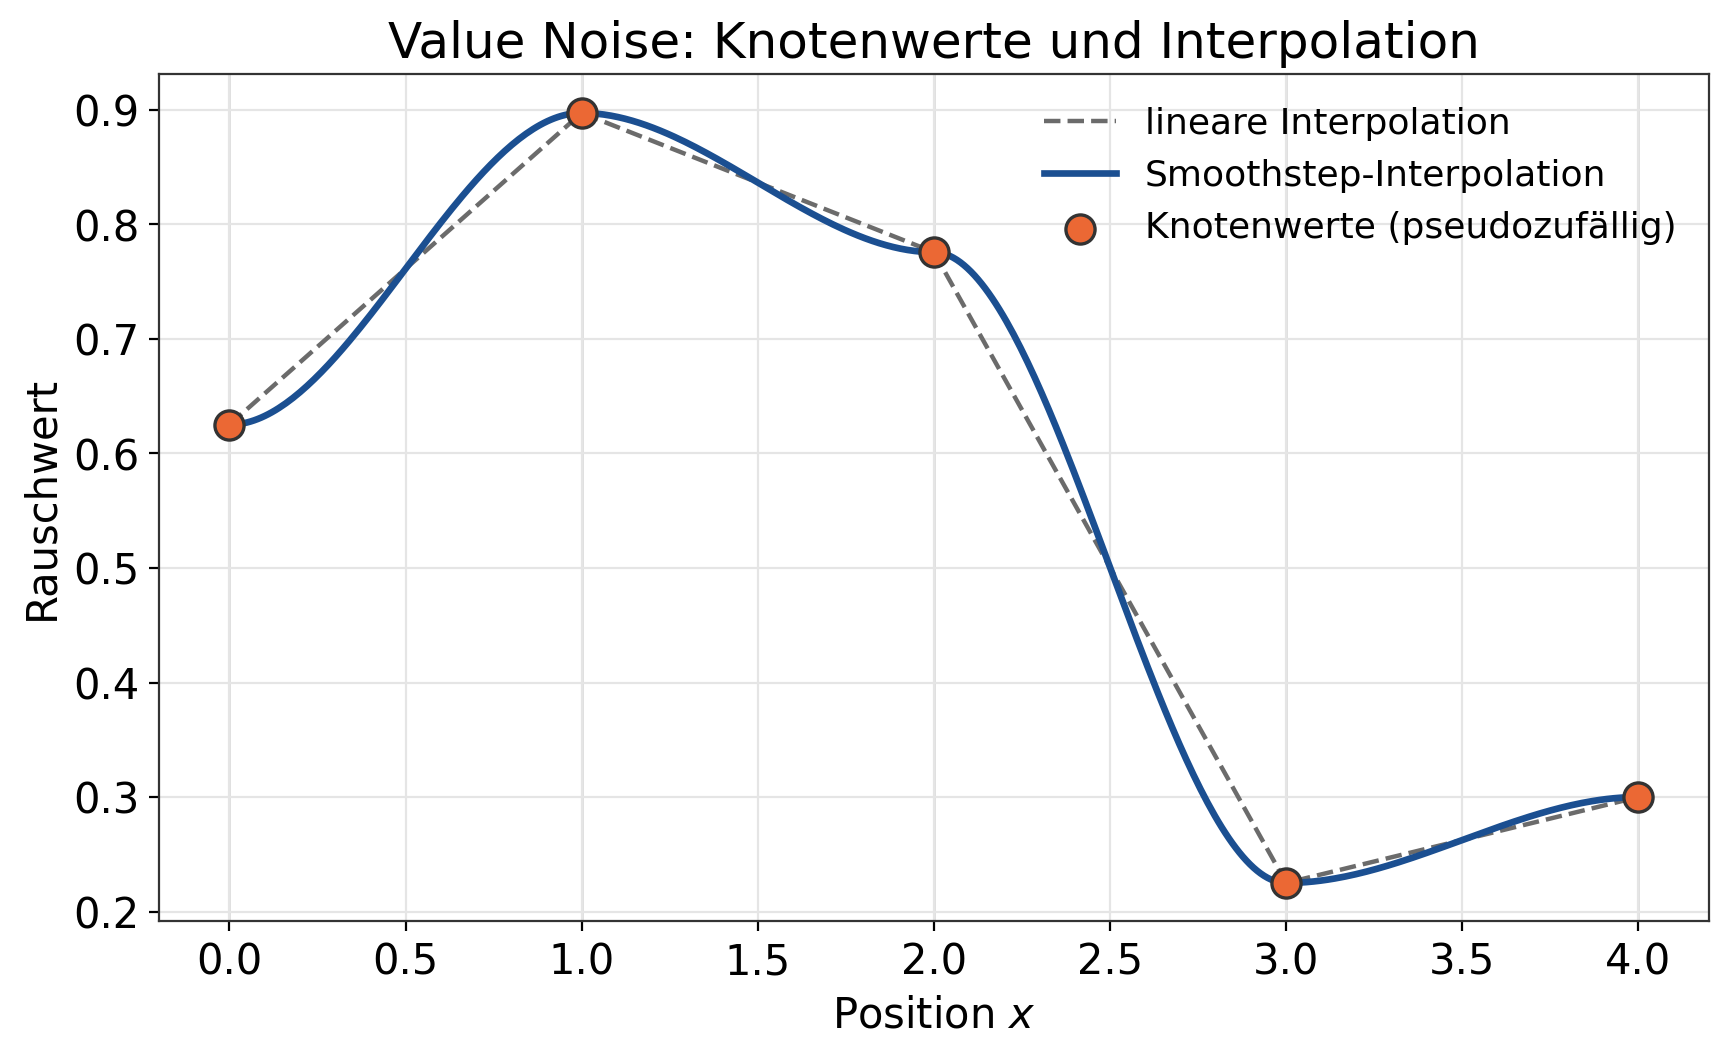
\includegraphics[width=0.75\textwidth]{Bilder/grundlagen_value_noise.png}
    \caption{Value Noise -- lineare gegen Smoothstep-Interpolation zwischen denselben Knotenwerten, eigene Darstellung.}
    \label{fig:grundlagen_value_noise}
\end{figure}

Im zweidimensionalen Raum erfolgt die Überlagerung der Interpolationen entlang beider Achsen mittels bilinearer Interpolation.

\subsubsection{Domain Warping und fraktale Akkumulation}
Um die typischen Raster-Artefakte einfacher Gitterstrukturen zu vermeiden, werden fortgeschrittene Techniken eingesetzt:

\begin{itemize}
    \item \textbf{Multi-Frequency / Fraktaler Noise:} Durch die Addition mehrerer Rauschfunktionen unterschiedlicher Frequenzen (Oktaven) und Amplituden lassen sich fraktalähnliche, hochdetaillierte Strukturen erzeugen. Niedrige Frequenzen steuern großflächige Formen (z.\,B. Kontinente), während hohe Frequenzen feine Details (z.\,B. Felsstrukturen) ergänzen.
    \item \textbf{Domain Warping} \citep{quilez_warp}: Hierbei werden die Eingangskoordinaten $(x, y)$ einer Rauschfunktion selbst durch den Ausgangswert einer anderen Rauschfunktion verzerrt:
    \begin{equation}
    f_{\text{warped}}(x, y) = f(x + g(x, y), y + h(x, y))
    \end{equation}
    Dies führt zu organischen Verformungen und eliminiert visuelle Gitterlinien.
\end{itemize}

Abbildung~\ref{fig:grundlagen_domain_warping} zeigt denselben Rauschausschnitt mit und ohne Domain Warping. Die verzerrte Variante rechts löst die diagonalen Vorzugsrichtungen des unverzerrten Rauschens auf und wirkt dadurch weniger regelmäßig.

\begin{figure}[htbp]
    \centering
    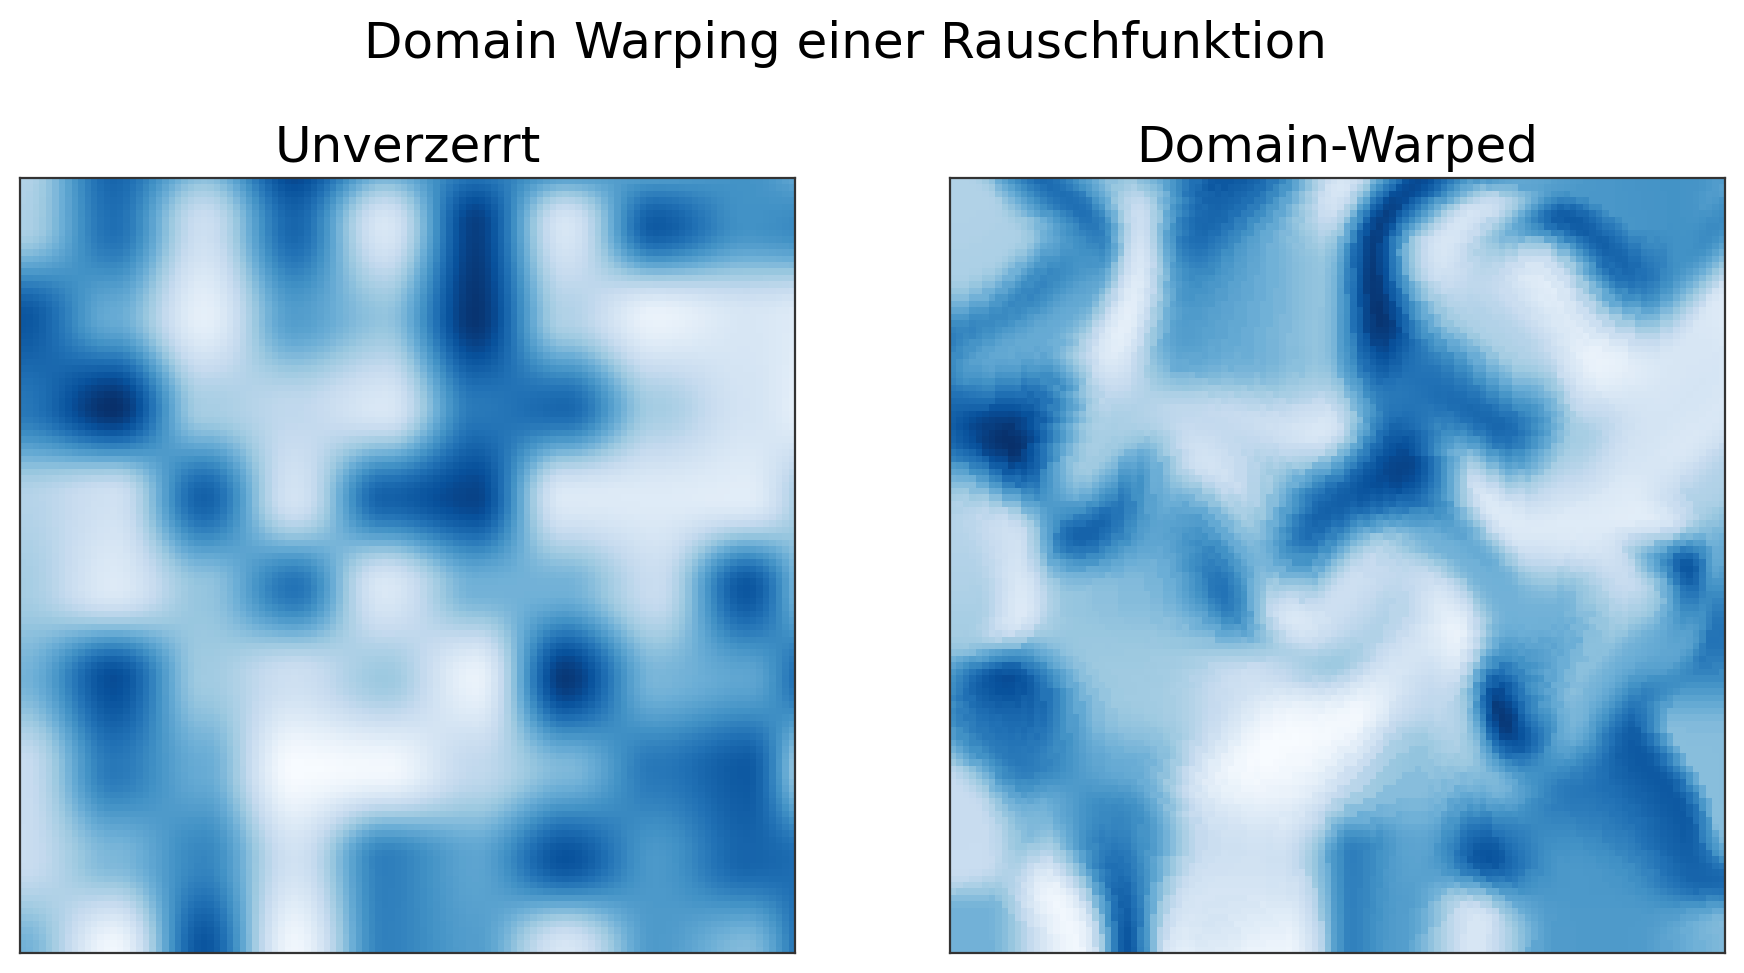
\includegraphics[width=0.85\textwidth]{Bilder/grundlagen_domain_warping.png}
    \caption{Domain Warping -- derselbe Rauschausschnitt unverzerrt und verzerrt, eigene Darstellung.}
    \label{fig:grundlagen_domain_warping}
\end{figure}

\subsection{Zelluläre Automaten zur Gefügeglättung}
\label{sec:grundlagen_ca}

Zelluläre Automaten (\textit{Cellular Automata}) bestehen aus Zellen, die diskrete Zustände (z.\,B. \textit{Wand} oder \textit{Freiraum}) annehmen können. In diskreten Zeitschritten aktualisiert jede Zelle ihren Zustand basierend auf einer lokalen Übergangsfunktion, welche die Zustände ihrer Nachbarschaft berücksichtigt.

Häufig wird hierbei die Moore-Nachbarschaft verwendet, welche die 8 direkt angrenzenden Zellen (horizontal, vertikal und diagonal) umfasst. Durch gezielte Geburts- und Überlebensregeln (\textit{Birth/Survival Rules}) lassen sich aus verrauschten Initialzuständen zusammenhängende, natürliche Höhlen- und Klippenstrukturen erzeugen, wie es für die prozedurale Erzeugung von Höhlenlevels bereits gezeigt wurde \citep{johnson2010cellular}. Abbildung~\ref{fig:grundlagen_ca} zeigt diesen Effekt an einem unabhängigen Beispielgitter mit der auch in der Projektkonfiguration hinterlegten Regel B5/S4 (Geburt ab 5, Überleben ab 4 Nachbarwänden): Aus unstrukturiertem Rauschen entstehen nach wenigen Iterationen zusammenhängende Flächen.

Im ausgelieferten Konfigurationsstand ist diese Nachbearbeitung deaktiviert (siehe Tabelle~\ref{tab:config_status}). Sie wird hier dennoch als Grundlage behandelt, weil sie die naheliegende algorithmische Alternative zum tatsächlich verwendeten Manhattan-Fallback markiert (siehe Abschnitt~\ref{sec:grundlagen_erreichbarkeit}) und dessen Auswahl erst vor diesem Hintergrund einordbar wird.

\begin{figure}[htbp]
    \centering
    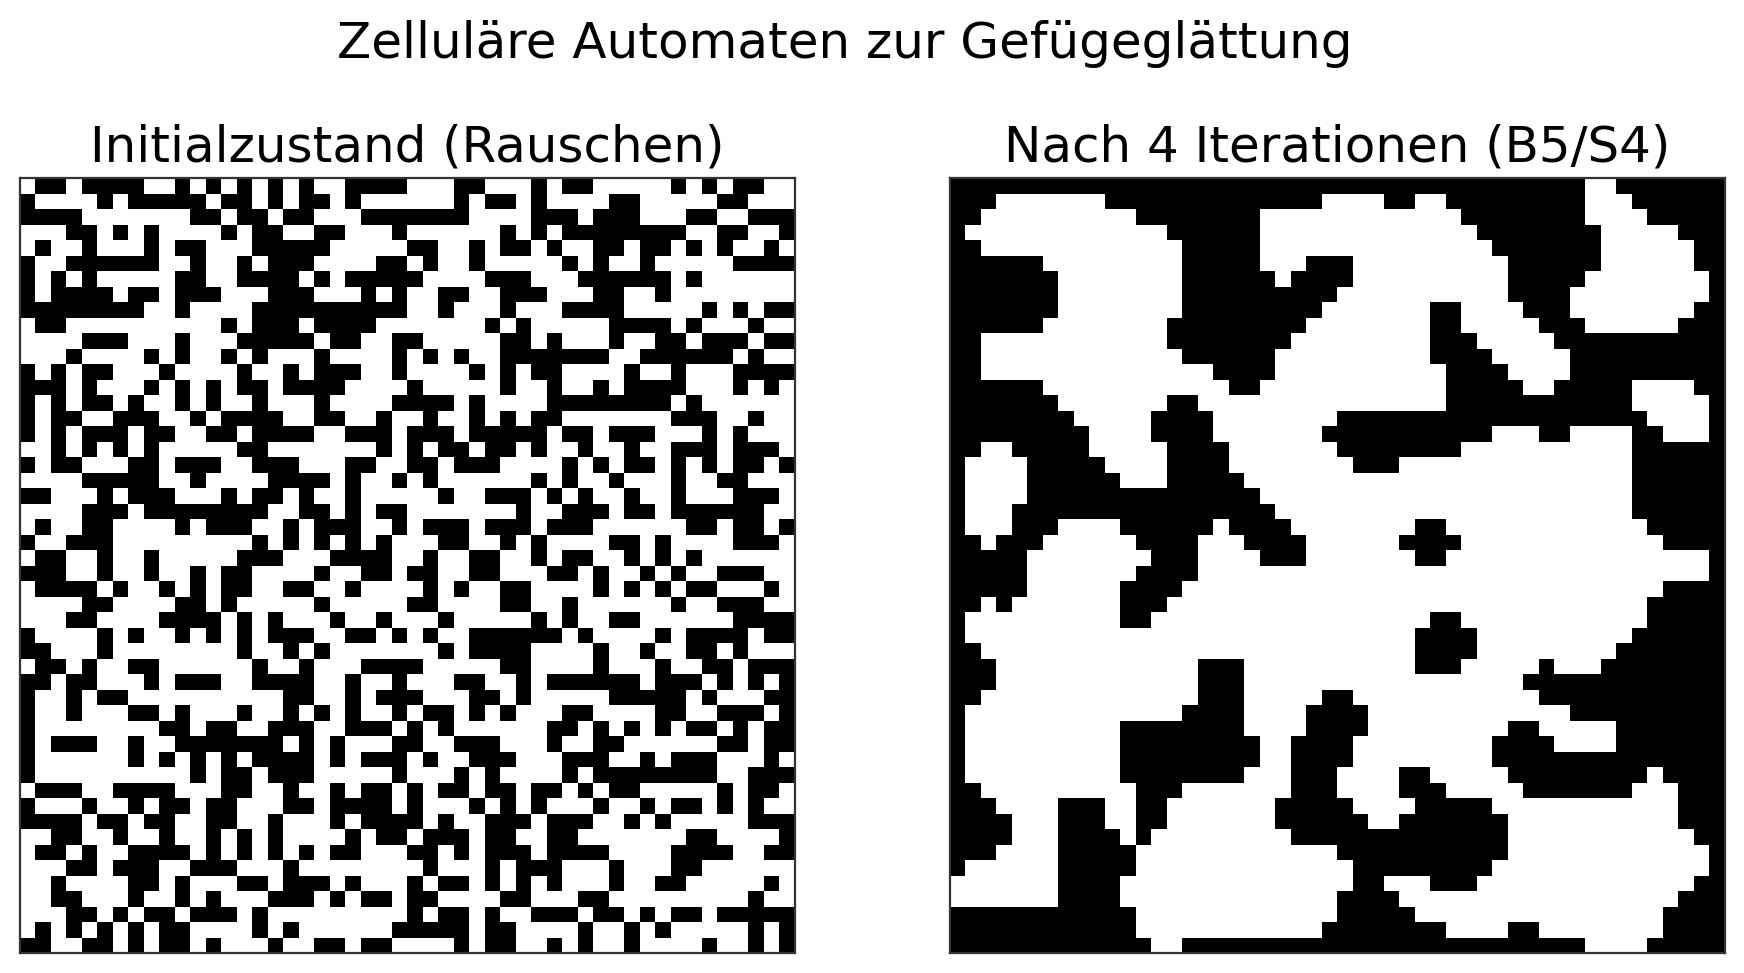
\includegraphics[width=0.85\textwidth]{Bilder/grundlagen_zellulaere_automaten.png}
    \caption{Zellulärer Automat -- Rauschgitter vor und nach vier Glättungsiterationen, eigene Darstellung.}
    \label{fig:grundlagen_ca}
\end{figure}

\subsection{Graphentheoretische Erreichbarkeitsanalyse}
\label{sec:grundlagen_erreichbarkeit}

Ein zentrales Kriterium prozeduraler Welten ist die Sicherstellung der Spielbarkeit, insbesondere die Vermeidung unlösbarer Level-Zustände (\textit{Deadlocks}).

\subsubsection{Breitensuche (Breadth-First Search, BFS)}
\label{sec:grundlagen_bfs}
Zur Analyse der Konnektivität wird das Zellgitter als ungerichteter Graph interpretiert, in dem begehbare Zellen als Knoten und Nachbarschaftsbeziehungen als Kanten dargestellt werden. Die Breitensuche (BFS) traversiert den Graphen ebenenweise vom Startknoten aus \citep{clrs2009algorithms}. Sie eignet sich zur Prüfung der Erreichbarkeit eines Zielknotens sowie zur Bestimmung des kürzesten Pfades auf ungewichten Gittern. Abbildung~\ref{fig:grundlagen_bfs} veranschaulicht das resultierende Distanzfeld an einem Beispielgitter: Jede Ebene entspricht einem BFS-Schritt vom Start aus, der kürzeste Pfad zum Ziel ergibt sich durch Rückverfolgung der jeweils näher liegenden Nachbarzelle.

Im ausgelieferten Konfigurationsstand dient die Breitensuche nicht mehr der Lösbarkeitsprüfung bei der Weltgenerierung (siehe Tabelle~\ref{tab:config_status}), da diese Rolle vollständig vom Manhattan-Fallback übernommen wird. Sie bleibt jedoch an anderer Stelle aktiv: als Distanzfeld für das Reward Shaping im RL-Training (Abschnitt~\ref{sec:impl_rl_reward}) und als Bezugsgröße der Pfadeffizienz-Metrik in der Evaluation (Abschnitt~\ref{sec:eval_eff}).

\begin{figure}[htbp]
    \centering
    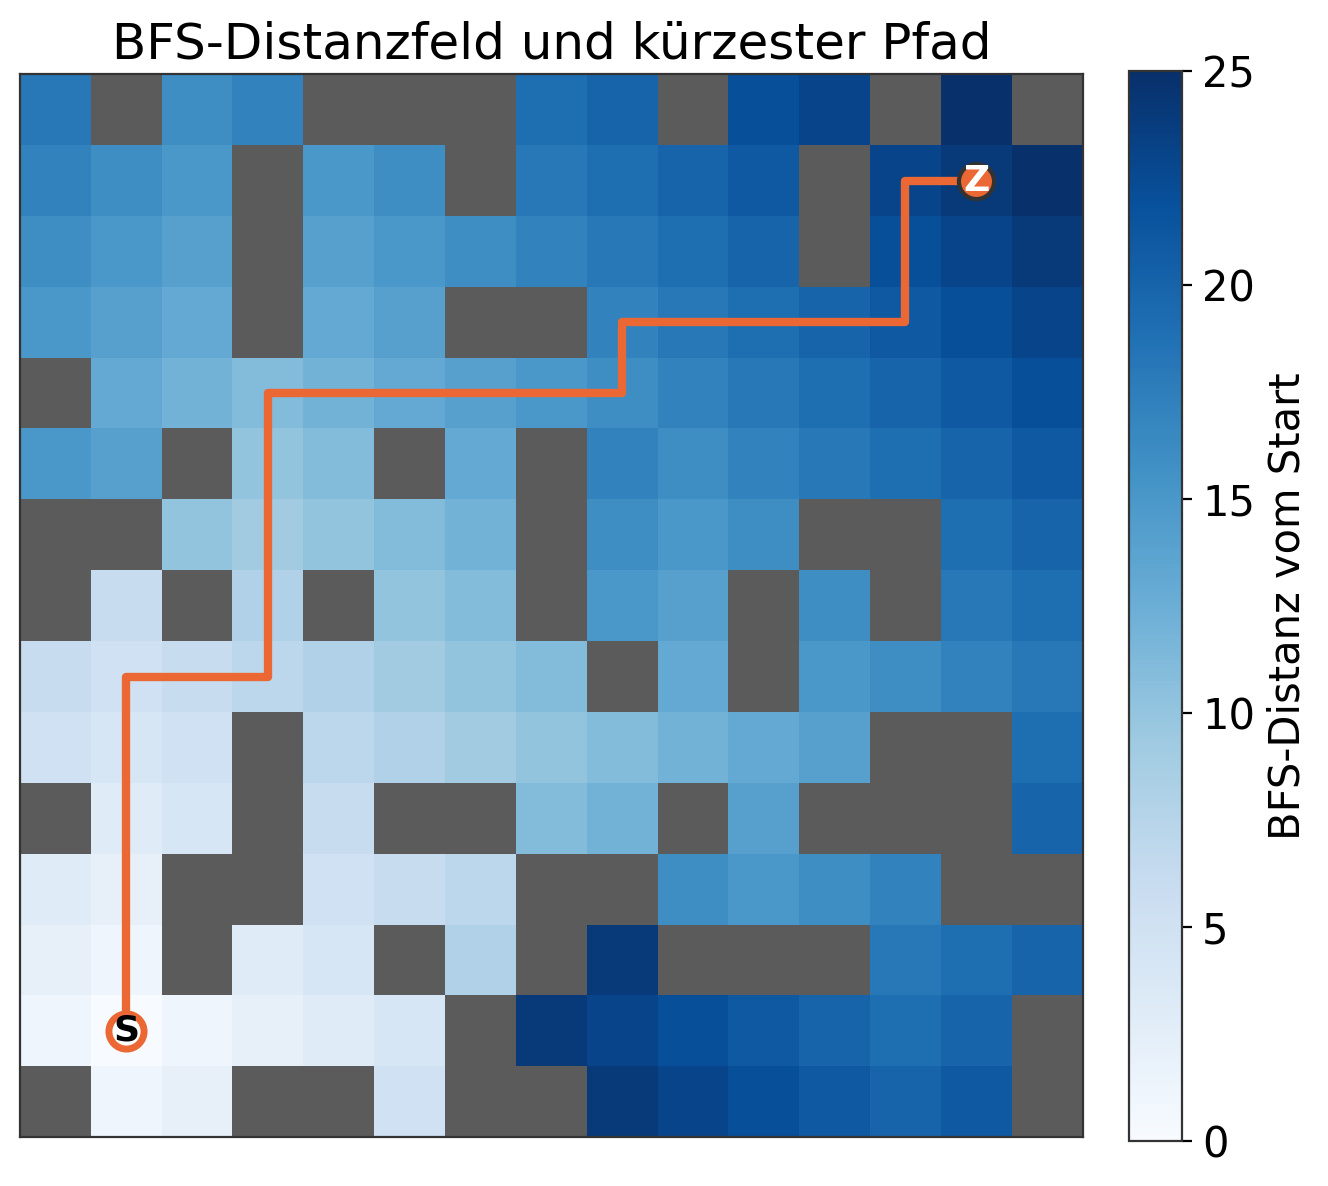
\includegraphics[width=0.55\textwidth]{Bilder/grundlagen_bfs.png}
    \caption{Breitensuche -- Distanzfeld vom Startpunkt und daraus resultierender kürzester Pfad, eigene Darstellung.}
    \label{fig:grundlagen_bfs}
\end{figure}

\subsubsection{Heuristische Validierung und Korrekturverfahren}
Da die exakte graphenbasierte Validierung bei großen Chunks rechenintensiv sein kann, werden in der Praxis häufig kombinierte Ansätze gewählt:
\begin{itemize}
    \item \textbf{Manhattan-Distanz:} Die Distanz zwischen zwei Punkten $(x_1, y_1)$ und $(x_2, y_2)$ auf einem orthogonalen Gitter berechnet sich nach:
    \begin{equation}
    D_{\text{Manhattan}} = |x_1 - x_2| + |y_1 - y_2|
    \end{equation}
    \item \textbf{Fallback-Generierung (Carving):} Sollte keine valide Verbindung existieren, stellen geometrische Ausgrabungsalgorithmen (\textit{Carving}) entlang direkter Achsen eine funktionale Wegeverbindung sicher.
\end{itemize}

\section{Grundlagen des Reinforcement Learning}
\label{sec:grundlagen_rl}

Das Reinforcement Learning (RL) ist ein Teilbereich des maschinellen Lernens, bei dem ein Agent lernt, durch Interaktion mit einer Umgebung optimale Entscheidungen zu treffen (siehe Abbildung \ref{fig:rl_interaktion}). Die formale mathematische Grundlage hierfür bildet der \textbf{Markov Decision Process (MDP)}. Ein MDP wird typischerweise als Tupel $(S, A, P, R, \gamma)$ definiert. Dabei steht $S$ für die Menge aller möglichen Zustände der Umgebung und $A$ für die Menge der möglichen Aktionen des Agenten. Die Übergangswahrscheinlichkeit $P(s' \mid s, a)$ beschreibt die Dynamik der Umgebung, also mit welcher Wahrscheinlichkeit der Agent durch die Aktion $a$ vom Zustand $s$ in den Folgezustand $s'$ gelangt. Für jeden dieser Übergänge erhält der Agent ein Feedback in Form eines numerischen Belohnungssignals, dem \textbf{Reward} $R(s, a)$. Das übergeordnete Ziel des Agenten ist es, eine Verhaltensregel, die sogenannte \textbf{Policy} $\pi(a \mid s)$, zu erlernen. Diese Policy ordnet jedem Zustand eine Aktion zu und maximiert dabei die erwartete, kumulierte Belohnung über die Zeit. Der Diskontierungsfaktor $\gamma \in [0, 1]$ bestimmt dabei, wie stark zukünftige Belohnungen im Vergleich zu unmittelbaren gewichtet werden \citep{sutton2018reinforcement}.

\begin{figure}[htbp]
    \centering
    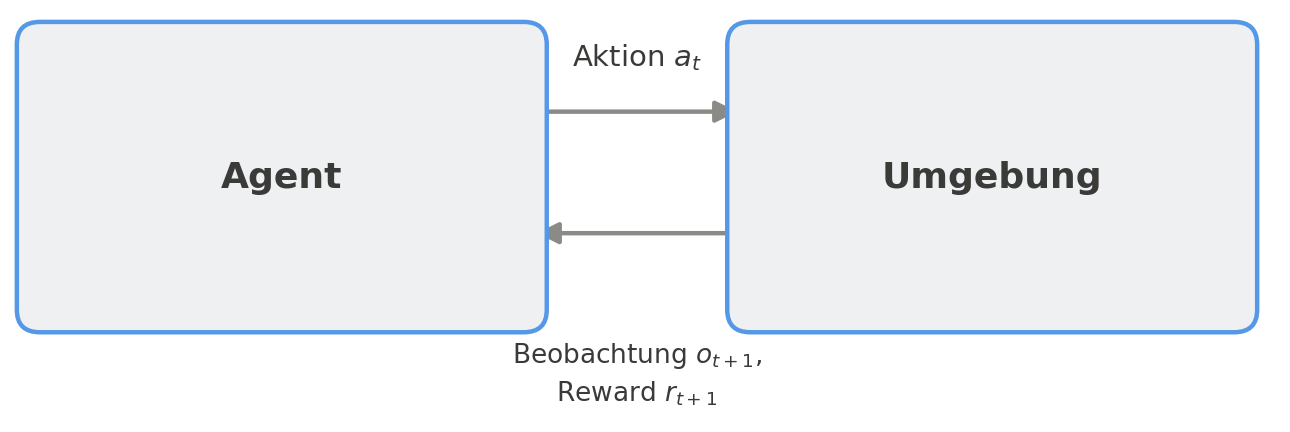
\includegraphics[width=0.85\textwidth]{Bilder/rl_interaktionsschleife.png}
    \caption{Interaktionsschleife zwischen Agent und Umgebung.}
    \label{fig:rl_interaktion}
\end{figure}

\subsection{Partially Observable Markov Decision Processes (POMDP)}
Die Standarddefinition des MDP geht von vollständiger Beobachtbarkeit aus. Der Agent kennt somit stets den exakten aktuellen Zustand $s$ der Umgebung. In vielen realen Szenarien ist diese Annahme jedoch nicht erfüllt, da Sensordaten verrauscht oder Informationen verborgen sein können. Für solche Problemstellungen wird das Konzept zum \textit{Partially Observable Markov Decision Process} (POMDP) erweitert. In einem POMDP hat der Agent keinen direkten Zugriff auf den wahren Zustand $s \in S$, sondern erhält lediglich eine Beobachtung $o \in \Omega$, die gemäß einer Beobachtungswahrscheinlichkeit $O(o \mid s, a)$ erzeugt wird (siehe Abbildung \ref{fig:mdp_pomdp}). Um dennoch optimale Entscheidungen treffen zu können, muss der Agent einen sogenannten \glqq Belief State\grqq{} (Überzeugungszustand) pflegen. Dieser stellt eine Wahrscheinlichkeitsverteilung über alle möglichen wahren Zustände der Umgebung dar und wird nach jeder neuen Aktion und Beobachtung kontinuierlich aktualisiert \citep{kaelbling1998planning}.

\begin{figure}[htbp]
    \centering
    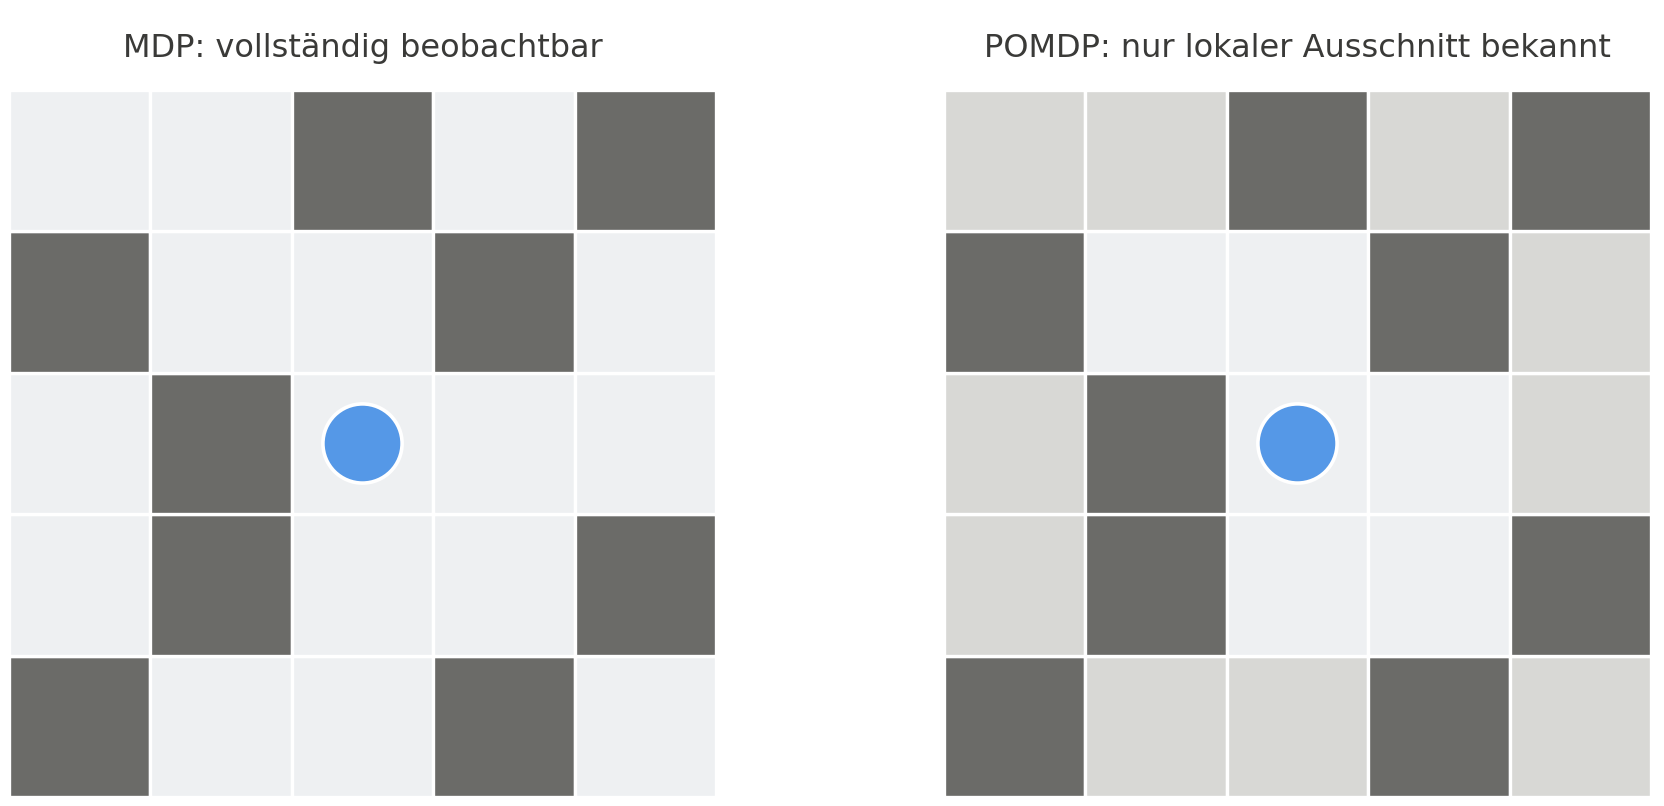
\includegraphics[width=0.85\textwidth]{Bilder/mdp_pomdp_vergleich.png}
    \caption{Vergleich zwischen vollständiger und partieller Beobachtbarkeit.}
    \label{fig:mdp_pomdp}
\end{figure}

\subsection{Potential Based Reward Shaping (PBRS)}
Eine zentrale Herausforderung im Reinforcement Learning sind verzögerte oder spärliche Belohnungen (Sparse Rewards), bei denen der Agent nur sehr selten ein positives Feedback erhält. Um den Lernprozess zu beschleunigen, wird häufig \textit{Reward Shaping} angewendet, bei dem das ursprüngliche Belohnungssignal durch zusätzliche, dichtere Zwischenbelohnungen angereichert wird. Die allgemeine Theorie des \textit{Potential Based Reward Shaping} (PBRS) löst dabei das Problem, dass naive Anpassungen der Belohnungsfunktion das eigentliche Ziel des Agenten verfälschen könnten (sogenanntes Reward Hacking). PBRS stellt mathematisch sicher, dass die optimale Policy des ursprünglichen MDPs trotz der zusätzlichen Belohnungen strikt erhalten bleibt. Dies wird erreicht, indem die formende Belohnung $F(s, a, s')$ als Differenz einer Potenzialfunktion $\Phi$ zwischen dem Folgezustand und dem aktuellen Zustand definiert wird (vergleiche Abbildung \ref{fig:pbrs_potential}): $F(s, a, s') = \gamma \Phi(s') - \Phi(s)$. Diese Funktion gibt dem Agenten kontinuierliches Feedback basierend auf seinem \glqq Abstand\grqq{} zum Ziel \citep{ng1999policy}.

\begin{figure}[htbp]
    \centering
    
\includegraphics[width=0.85\textwidth]{Bilder/pbrs_potentialfeld.png}
    \caption{Veranschaulichung des Potentialfelds $\Phi(s)$ und der daraus resultierenden formenden Belohnung entlang eines Beispielpfads.}
    \label{fig:pbrs_potential}
\end{figure}

\subsection{Curriculum Learning}
Wenn Aufgaben für einen untrainierten RL Agenten zu komplex sind, schlägt das Lernen oft vollständig fehl, da der Agent rein durch zufällige Exploration keine Lösung findet. Das allgemeine Prinzip des \textit{Curriculum Learning} greift dieses Problem auf, indem es sich an der menschlichen Pädagogik orientiert: Anstatt dem Agenten sofort die finale, hochkomplexe Aufgabe zu stellen, wird der Lernprozess strukturiert. Der Agent trainiert zunächst auf stark vereinfachten Versionen der Aufgabe. Sobald er diese beherrscht, wird der Schwierigkeitsgrad der Umgebung oder der Aufgabenstellung schrittweise erhöht, bis die Zieldomäne erreicht ist. Diese methodische Abfolge (das Curriculum) beschleunigt nicht nur die Konvergenz des Lernalgorithmus erheblich, sondern ermöglicht es oft erst, dass der Agent für sehr komplexe Problemstellungen überhaupt eine optimale Policy findet \citep{bengio2009curriculum, narvekar2020curriculum}.

\subsection{Proximal Policy Optimization (PPO)}
Proximal Policy Optimization (PPO) gehört zur Familie der Policy Gradient Methoden und wurde von \citet{schulman2017proximal} als Weiterentwicklung etablierter Verfahren wie der Trust Region Policy Optimization (TRPO) eingeführt. Der zentrale Vorteil von PPO liegt in der Balance zwischen einfacher Implementierung, hoher Stichprobeneffizienz (Sample Efficiency) und Trainingsstabilität. Während herkömmliche Methoden des Policy Gradient bei zu großen Aktualisierungsschritten destabilisieren und die erlernte Verhaltensregel ruinieren können, führt PPO eine sogenannte Clippingfunktion (\textit{Clipped Surrogate Objective}) ein (vergleiche Abbildung \ref{fig:ppo_clip}). Diese Zielfunktion beschränkt die Änderungen der Policy zwischen zwei aufeinanderfolgenden Trainingsschritten auf ein definiertes Intervall, meist parametrisiert durch einen Hyperparameter $\epsilon$ (zum Beispiel $[1-\epsilon, 1+\epsilon]$). Dadurch wird mathematisch verhindert, dass der Agent seine Strategie in einem einzelnen Updateschritt zu drastisch ändert. Dies führt zu einer monotoneren Verbesserung und einem wesentlich robusteren Lernverhalten, ohne den hohen rechnerischen Aufwand, der bei TRPO für die Berechnung der Kullback Leibler Divergenz anfällt \citep{schulman2017proximal}.

\begin{figure}[htbp]
    \centering
    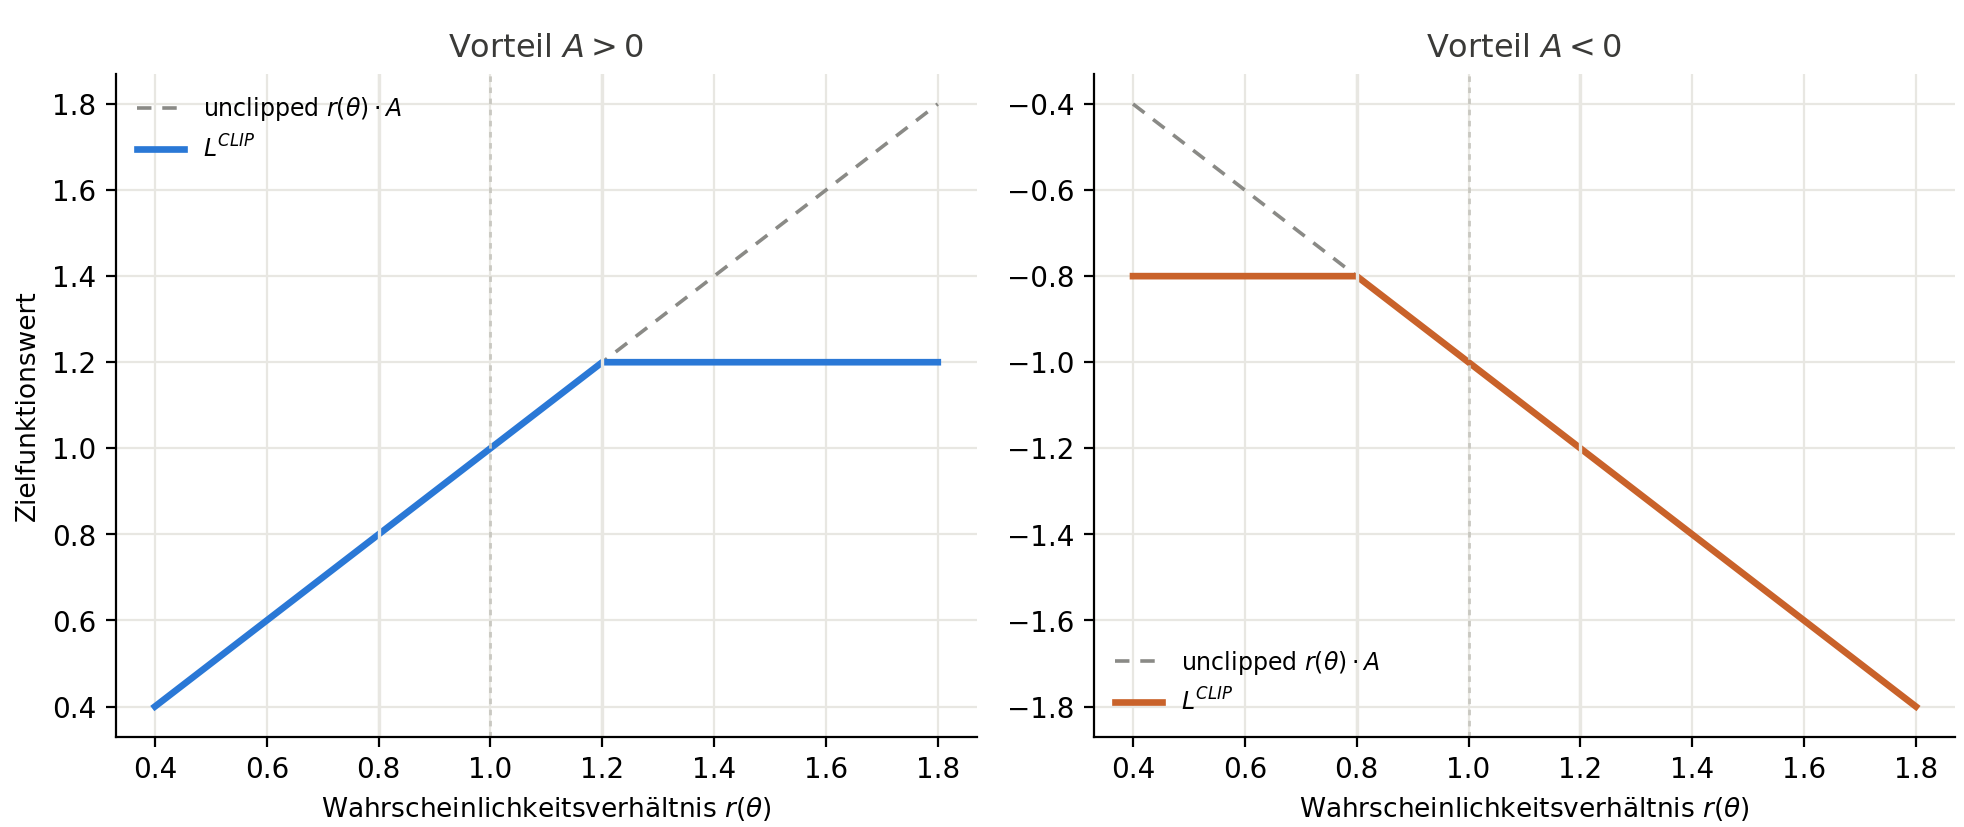
\includegraphics[width=0.85\textwidth]{Bilder/ppo_clipped_objective.png}
    \caption{Darstellung der Clipped Surrogate Objective von PPO.}
    \label{fig:ppo_clip}
\end{figure}

\subsection{Rekurrente Neuronale Netze (RNN)}
Wie in der Definition der POMDPs beschrieben, kann ein Agent in Umgebungen mit partieller Beobachtbarkeit den wahren Zustand nicht aus einer einzelnen, isolierten Beobachtung ableiten. Um dieses Problem zu überwinden, muss der Agent auf vergangene Beobachtungen zurückgreifen können, wofür rekurrente neuronale Netze (RNNs) eingesetzt werden. Im Gegensatz zu zustandslosen Netzwerken (Feedforward Netzen) besitzen RNNs einen internen Speicher, der bei jedem Zeitschritt basierend auf der aktuellen Eingabe und dem vorherigen Zustand aktualisiert wird. Durch diesen impliziten Gedächtnisaufbau kann das Netzwerk die verborgenen Zustandsinformationen eines POMDPs aus der Historie der Beobachtungen näherungsweise rekonstruieren. Eine rekurrente Policy ist somit in der Lage, auch dann optimale Entscheidungen zu treffen, wenn das aktuelle Beobachtungssignal allein keine eindeutige Zustandsschätzung zulässt \citep{hausknecht2015deep}. Ein grundlegendes Problem einfacher RNNs ist jedoch das Phänomen des verschwindenden Gradienten (\textit{Vanishing Gradient}), wodurch das Netzwerk große Schwierigkeiten hat, Abhängigkeiten über längere Zeiträume stabil zu erlernen.

\subsection{Long Short Term Memory (LSTM)}
Um das Problem des verschwindenden Gradienten zu lösen, bildet die \textit{Long Short Term Memory} Architektur die fundamentale Basis für moderne rekurrente Netze. Sie wurde von \citet{hochreiter1997long} entwickelt und stellt eine spezialisierte Form von RNNs dar. LSTMs nutzen ein System aus dedizierten Speicherzellen und Gatingmechanismen (Input Gates, Output Gates und Forget Gates). Diese Struktur ermöglicht es dem Netzwerk gezielt zu steuern, welche relevanten Informationen über lange Zeitreihen hinweg gespeichert, aktualisiert oder vergessen werden sollen. Für das Reinforcement Learning ist dies von entscheidender Bedeutung: Der Agent kann dadurch wichtige Ereignisse, die viele Schritte in der Vergangenheit liegen, verlustfrei in seinem Gedächtnis behalten und für aktuelle Entscheidungen heranziehen (siehe Abbildung \ref{fig:rnn_policy}). Die Integration von LSTM Zellen ermöglicht es dem Agenten somit, Sequenzen von Beobachtungen über die Zeit effektiv zu aggregieren und komplexe Aufgaben in unvollständig beobachtbaren Umgebungen erfolgreich zu lösen \citep{hochreiter1997long, hausknecht2015deep}.

\begin{figure}[htbp]
    \centering
    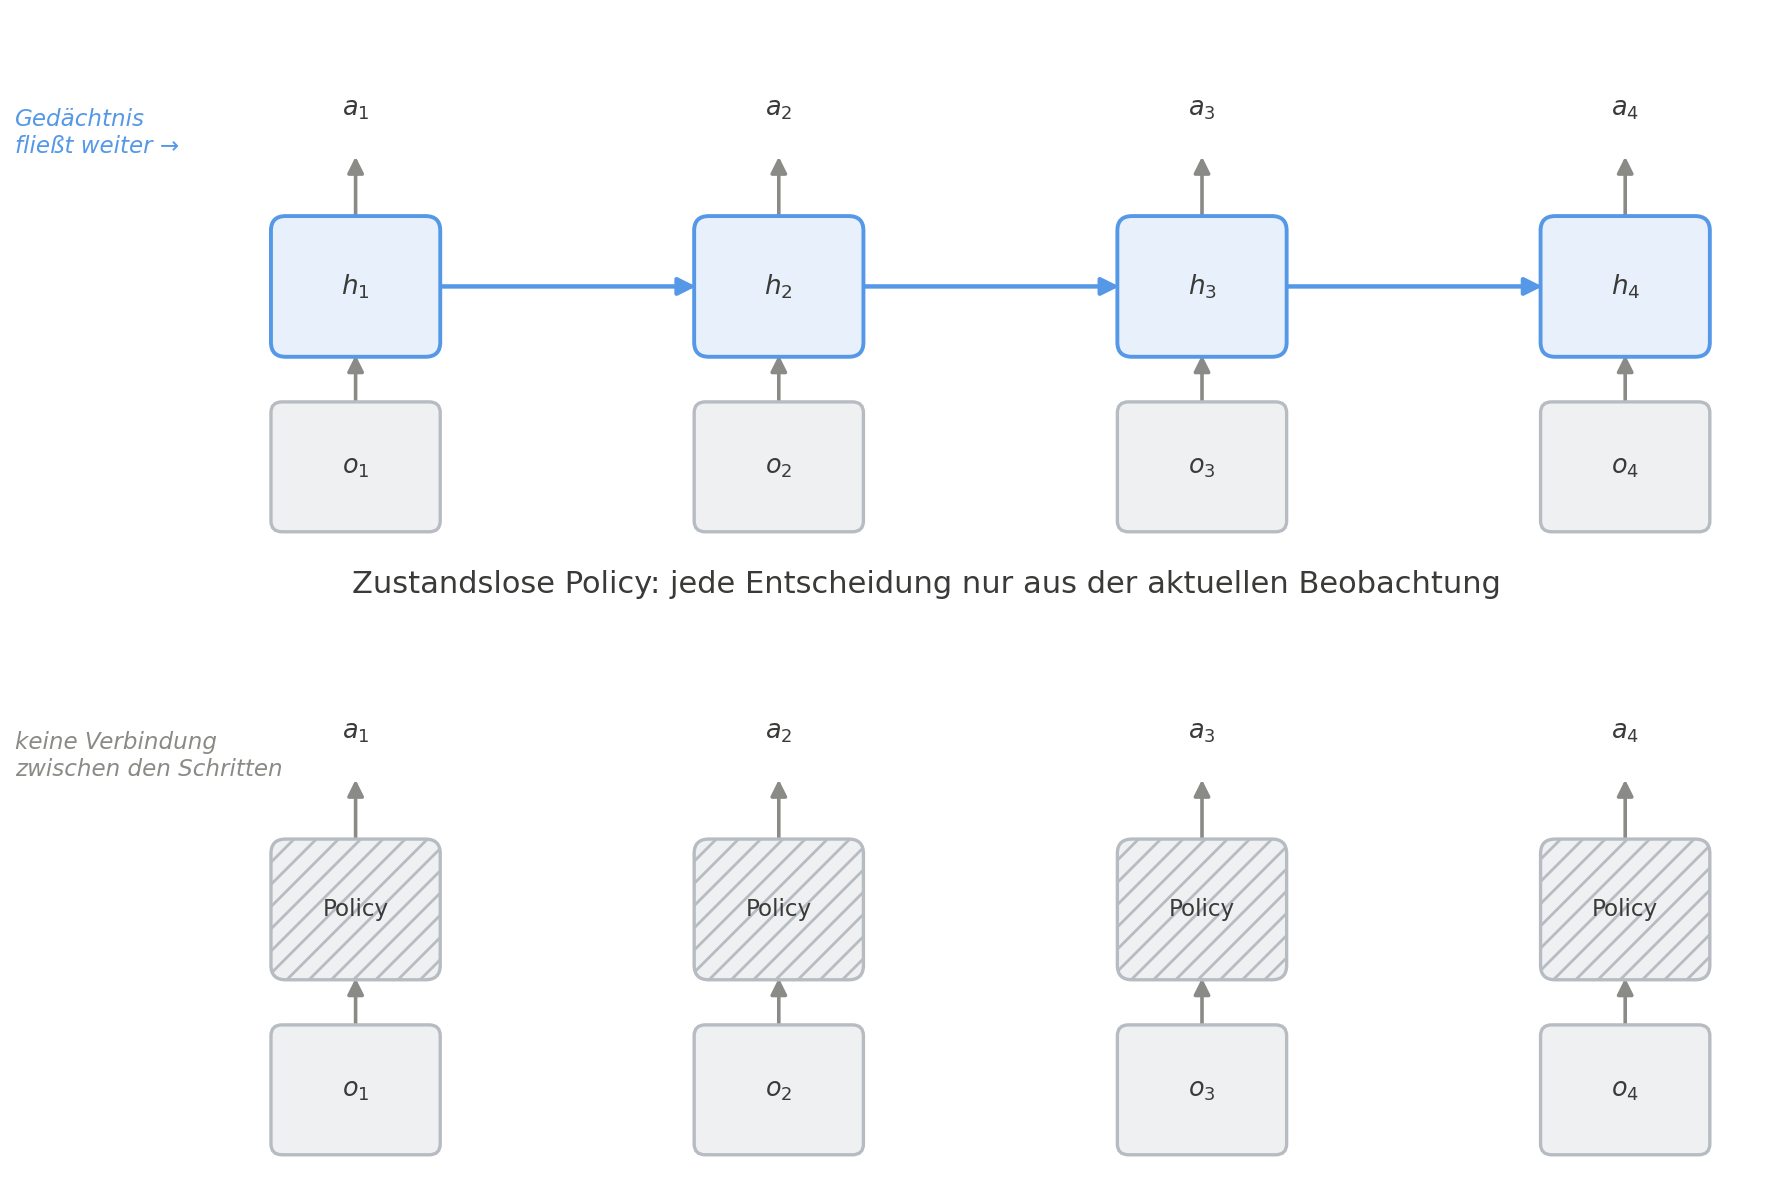
\includegraphics[width=0.85\textwidth]{Bilder/rekurrente_policy_schema.png}
    \caption{Funktionsweise einer rekurrenten Policy im Vergleich zu einer zustandslosen Policy.}
    \label{fig:rnn_policy}
\end{figure}

\subsection{Deep Q Networks (DQN)}
Deep Q Networks (DQN) stellen einen entscheidenden Meilenstein in der Entwicklung des modernen Reinforcement Learning dar und wurden maßgeblich durch \citet{mnih2015human} geprägt. Im Gegensatz zu den zuvor beschriebenen Methoden des Policy Gradient handelt es sich bei DQN um einen wertebasierten Ansatz. Anstatt die Policy direkt zu parametrisieren, approximiert ein tiefes neuronales Netz die sogenannte Q Funktion (Action Value Funktion). Diese Funktion schätzt die erwartete kumulierte Belohnung für eine spezifische Aktion in einem bestimmten Zustand. Da die Kombination von klassischem Q Learning mit nichtlinearen Funktionsapproximatoren wie neuronalen Netzen historisch oft zu starker Instabilität und Divergenz im Lernverhalten führte, führte DQN zwei zentrale Innovationen ein (siehe Abbildung \ref{fig:dqn_architektur}). Zum einen das \textit{Experience Replay}, bei dem vergangene Interaktionen des Agenten kontinuierlich in einem Ringpuffer gespeichert und während des Trainings in zufälligen Batches wiederverwendet werden. Dies bricht die zeitliche Korrelation der Trainingsdaten auf und glättet die Datenverteilung. Zum anderen wird ein separates \textit{Target Network} genutzt, dessen Parameter im Gegensatz zum primären Netzwerk nur periodisch aktualisiert werden. Dies hält die Zielwerte für die Fehlerberechnung über mehrere Trainingsschritte hinweg konstant und verhindert Aufschaukelungseffekte. Durch diese beiden Mechanismen ermöglichte DQN erstmals das stabile Erlernen komplexer Verhaltensstrategien direkt aus hochdimensionalen Beobachtungen \citep{mnih2015human}.

\begin{figure}[htbp]
    \centering
    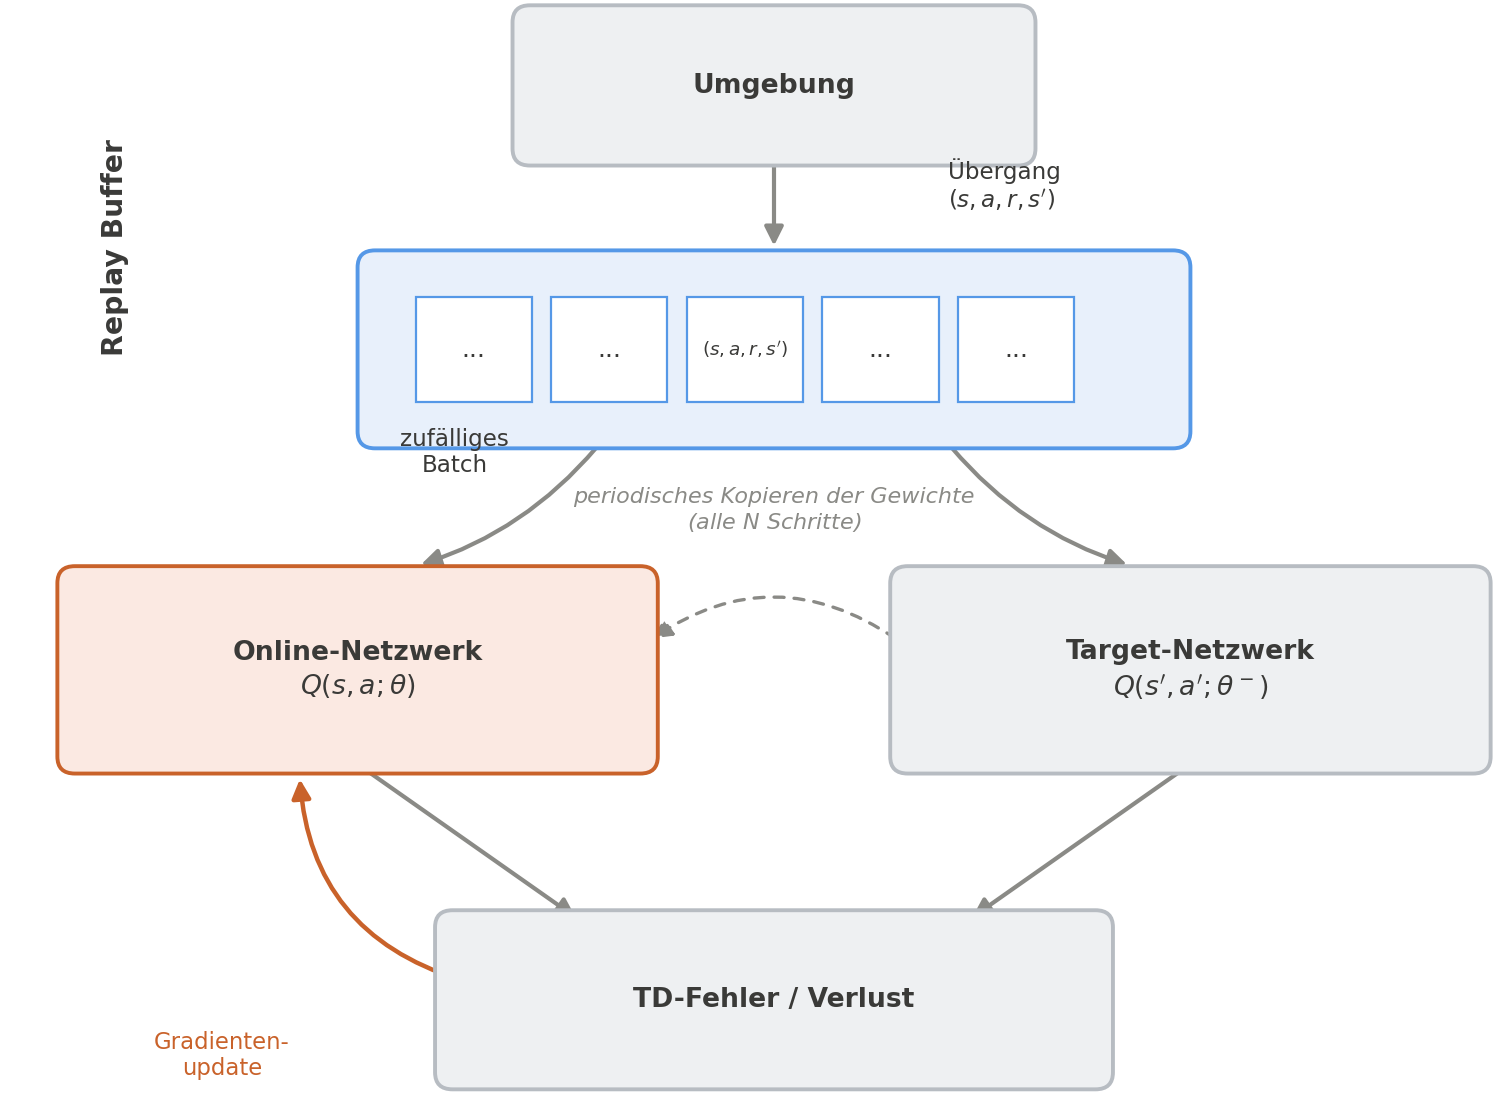
\includegraphics[width=0.85\textwidth]{Bilder/dqn_architektur.png}
    \caption{Zusammenspiel von Replay Buffer und Target Network in der DQN Architektur.}
    \label{fig:dqn_architektur}
\end{figure}

\subsection{Die Gymnasium-Schnittstelle (ehemals OpenAI Gym)}
\label{sec:grundlagen_gymnasium}
Um Reinforcement-Learning-Algorithmen unabhängig von der konkreten Problemstellung entwickeln und testen zu können, bedarf es einer standardisierten Kommunikationsschicht zwischen dem lernenden Agenten und der simulierten Welt. In der Forschung und Industrie hat sich hierfür ein dominanter Standard etabliert, der ursprünglich 2016 von OpenAI unter dem Namen \glqq Gym\grqq\ veröffentlicht wurde \cite{brockman2016openai}. Um die langfristige Wartung und Weiterentwicklung zu sichern, wurde das Projekt Ende 2022 an die gemeinnützige Farama Foundation übergeben und wird seitdem unter dem Namen \glqq Gymnasium\grqq\ fortgeführt \cite{towers2023gymnasium}.

Die Kernidee von Gymnasium ist die strikte Entkopplung: Der Algorithmus muss nicht wissen, ob er ein Videospiel spielt, einen Roboter steuert oder eine Lagerhalle optimiert. Die Umgebung (\texttt{Environment} oder kurz \texttt{Env}) kapselt die gesamte interne Logik, Physik und Zustandsspeicherung und gibt nach außen hin nur eine simple, wohldefinierte Programmierschnittstelle (API) preis. Diese API modelliert exakt den in der Theorie definierten Markov-Entscheidungsprozess (MDP) über folgende Hauptkomponenten:

\textbf{Definition der Zustands- und Aktionsräume}
Bevor das Training beginnt, muss der Agent wissen, welche Sensordaten er empfängt und welche Knöpfe er drücken kann. Gymnasium definiert dafür sogenannte \texttt{spaces}:
\begin{itemize}
    \item \texttt{observation\_space}: Definiert das Format und die Wertebereiche der Beobachtungen, die die Umgebung zurückgibt (z.\,B. ein mehrdimensionaler Vektor für Kamerabilder oder Sensordaten, repräsentiert als \texttt{Box}-Raum).
    \item \texttt{action\_space}: Definiert die erlaubten Aktionen, beispielsweise diskrete Eingaben (hoch, runter, links, rechts) als \texttt{Discrete}-Raum oder kontinuierliche Werte für Motoren als \texttt{Box}-Raum.
\end{itemize}

\textbf{Der Interaktionszyklus (\texttt{reset} und \texttt{step})}
Die eigentliche Interaktion verläuft zyklisch und wird über zwei zentrale Funktionen gesteuert:
\begin{itemize}
    \item \texttt{reset()}: Setzt die Umgebung in einen initialen Startzustand zurück und liefert die allererste Beobachtung an den Agenten. Dies markiert den Beginn einer neuen Episode.
    \item \texttt{step(action)}: Der Agent übergibt seine gewählte Aktion an die Umgebung. Die Umgebung simuliert daraufhin genau einen Zeitschritt und gibt ein Tupel (früher vier, in der aktuellen Gymnasium-Version fünf Werte) zurück:
    \begin{itemize}
        \item \texttt{observation}: Die neue Beobachtung des resultierenden Zustands ($s_{t+1}$).
        \item \texttt{reward}: Die skalare Belohnung ($r_{t+1}$) für die ausgeführte Aktion.
        \item \texttt{terminated}: Ein boolescher Wahrheitswert, der angibt, ob die Episode durch einen regulären Endzustand (z.\,B. Ziel erreicht oder \glqq Game Over\grqq) beendet wurde.
        \item \texttt{truncated}: Ein boolescher Wahrheitswert, der angibt, ob die Episode künstlich von außen abgebrochen wurde (z.\,B. weil ein Zeitlimit bzw. eine maximale Schrittzahl erreicht wurde).
        \item \texttt{info}: Ein Dictionary für zusätzliche Diagnose- und Metrikinformationen, die für das eigentliche Training irrelevant, aber für die Auswertung nützlich sind.
    \end{itemize}
\end{itemize}

Durch diese standardisierte Abstraktion ist es möglich, komplexe, eigens in C++ oder anderen performanten Sprachen geschriebene Simulationen über einen Python-Wrapper als \texttt{gymnasium.Env} bereitzustellen. Moderne RL-Frameworks wie Stable-Baselines3 \cite{raffin2021stable} erwarten exakt diese Schnittstelle und können so ohne weitere Anpassungen direkt auf der individuellen Umgebung trainieren.

%%%%%%%%%%%%%%%%%%%%%%%%%%%%%%%%%%%%%%%%%%%%%%%%%%%%%%%%%%%%%%%%
% BEGIN: kapitel/03_methodik.tex
%%%%%%%%%%%%%%%%%%%%%%%%%%%%%%%%%%%%%%%%%%%%%%%%%%%%%%%%%%%%%%%%
\chapter{Methodik}
\label{chap:methodik}

\section{Methodik der Weltgenerierung}
\label{sec:konzept_procedural}

Dieses Kapitel beschreibt die Architektur der prozeduralen Weltengenerierung. Das System kombiniert deterministische Rauschfunktionen zur Landschaftserzeugung mit regelbasierten Heuristiken zur Gewährleistung der Spielbarkeit.

\subsection{Methodische Grundlagen}
\label{sec:fundierung}

Die Generierung nutzt einen initialen Seed als Basis für alle pseudozufälligen Operationen, um Welten reproduzierbar zu berechnen.

\subsubsection{Pseudozufall und Rauscherzeugung}
Zur zustandslosen Berechnung von Raumkoordinaten $(x, y)$ transformiert eine Hash-Funktion die Koordinaten, den Welt-Seed und ein Salt in einen normalisierten Zufallswert im Intervall $[0, 1]$ (\texttt{world.cpp}, Z.~111–120).

Für zusammenhängende Strukturen wird ein \textit{Value-Noise}-Verfahren verwendet (\texttt{world.cpp}, Z.~131), dessen theoretische Grundlage bereits vorgestellt wurde (siehe Kapitel~2.1.2). Die Werte der vier Eckpunkte einer Gitterzelle werden ermittelt und bilinear interpoliert (\texttt{world.cpp}, Z.~149). Zur Kantenenglättung wird der Interpolationsparameter $t \in [0, 1]$ zuvor über die Smoothstep-Funktion transformiert:

\begin{equation}
S(t) = 3t^2 - 2t^3
\end{equation}

\subsubsection{Domain Warping und fraktaler Noise}
Um sichtbare Rasterstrukturen des quadratischen Gitters zu brechen, verzerrt ein vorgeschaltetes Rauschen die Eingangskoordinaten (\textit{Domain Warping}; \texttt{world.cpp}, Z.~163). Mehrere Rauschfunktionen unterschiedlicher Frequenzen und Amplituden werden aufaddiert (fraktaler Noise), um feiner strukturierte Umgebungen zu erzeugen (\texttt{world.cpp}, Z.~167).

\subsubsection{Nachbearbeitung und Validierung}
Die generierten Chunks können optional mittels zellulärer Automaten nachbearbeitet werden (\texttt{world.cpp}, Z.~487). Die Geburts- und Überlebensregeln der Moore-Nachbarschaft werden über die Konfiguration gesteuert (\texttt{game\_config.cpp}, Z.~155).

Zur topologischen Prüfung dient eine Breitensuche (Breadth-First Search, BFS) (siehe Kapitel~2.1.4). Sie verifiziert die Erreichbarkeit innerhalb des Chunks (\texttt{world.cpp}, Z.~555) sowie valide Ausgänge in einem definierten Distanzring (\texttt{world.cpp}, Z.~328).

\subsection{Heuristiken und Regeln}
\label{sec:heuristiken}

\subsubsection{Biome und Schwellenwerte}
Die Welt wird über ein Binning des Rauschergebnisses in festen Intervallen von $\frac{1}{7}$ in sieben Biome unterteilt (\texttt{world.cpp}, Z.~173). Biomspezifische Schwellenwerte steuern das Platzieren von Hindernissen, Erzen und Vegetation (\texttt{world.cpp}, Z.~412).

Gewässer entstehen durch eine gewichtete Linearkombination zweier Rauschfunktionen:
\begin{equation}
\text{Score} = 0,75 \cdot a + 0,25 \cdot b
\end{equation}
Zellen mit einem Wert über $0,86$ werden als Wasser markiert (\texttt{world.cpp}, Z.~308).

\subsubsection{Freiräume und Fallback-Pfade}
Um unspielbare Zustände zu vermeiden, gräbt ein Fallback-Algorithmus bei Bedarf einen direkten Manhattan-Pfad (zuerst X-, dann Y-Achse) in die Karte (\texttt{world.cpp}, Z.~655). Feste Radien um Spawn- und Zielpunkte verhindern das Blockieren der Start- und Endpositionen (\texttt{world.cpp}, Z.~20, Z.~677).

Point-of-Interest-Strukturen werden mit einer Wahrscheinlichkeit von $P = 0,10$ pro Chunk platziert (\texttt{world.cpp}, Z.~219). Ihre Form basiert auf biomspezifischen $5 \times 5$ ASCII-Matrizen (\texttt{world.cpp}, Z.~239).

\subsection{Systemkonfiguration}
\label{sec:konfiguration}

Die Parameter \texttt{coldBiomeMax} und \texttt{warmBiomeMax} in \texttt{game\_config.cpp} (Z.~124) werden zwar eingelesen, sind jedoch durch das feste $\frac{1}{7}$-Binning funktional obsolet.

Der aktuelle Standard-Betriebsmodus laut \texttt{game\_config.json}:

\begin{table}[h!]
\centering
\caption{Konfigurationsstatus der Weltengenerierung}
\label{tab:config_status}
\begin{tabular}{lll}
\hline
\textbf{Feature / Algorithmus} & \textbf{Status} & \textbf{Referenz} \\ \hline
Zelluläre Automaten (CA)       & DEAKTIVIERT     & \texttt{game\_config.json}, Z.~25 \\
Erreichbarkeitstest (BFS)      & DEAKTIVIERT     & \texttt{game\_config.json}, Z.~25 \\
Garantierter Pfad (Manhattan)  & AKTIVIERT       & \texttt{game\_config.json}, Z.~7  \\ \hline
\end{tabular}
\end{table}

In der Praxis sichert somit primär der Manhattan-Fallback die Wegeverbindung, während rechenintensive Validierungen deaktiviert sind.
\section{Methodik des RL-Trainings}
\label{sec:methodik_rl}

Dieses Kapitel behandelt die methodische Umsetzung der zweiten Forschungsfrage: Wie gut können rekurrente (LSTM) und zustandslose (MLP) PPO-Agenten navigieren, wenn die Umgebung nur teilweise sichtbar ist (partielle Beobachtbarkeit)? Dafür wird im Folgenden das Setup für das Reinforcement Learning (RL) beschrieben, also die Problemformulierung, das Curriculum, die Validierung und der genaue Evaluationsablauf. Die reinen technischen Details zur Implementierung folgen separat in Kapitel~4.2.

\subsection{Auswahl der zu vergleichenden Trainingsverfahren}
\label{sec:methodik_auswahl}

Im Mittelpunkt des Vergleichs stehen zwei Varianten der Proximal Policy Optimization (PPO): eine mit rekurrenter LSTM-Policy (im Folgenden LSTM-PPO) und eine mit zustandsloser Multilayer-Perceptron-Policy (MLP-PPO). Da beide Modelle den gleichen grundlegenden Optimierungsmechanismus nutzen, lässt sich durch diesen Aufbau gut untersuchen, welchen Einfluss das Gedächtnis (Rekurrenz) auf die Navigation in solchen Umgebungen hat. 

Frühere Tests mit Deep Q-Networks (DQN) wurden für diese Untersuchung verworfen. Erste Analysen zeigten, dass die gelernten Q-Werte für alle vier Aktionen extrem nah beieinander lagen (zwischen 0,12 und 0,38). Dadurch konnte der Agent keine klare Richtung lernen und hing oft in endlosen Pendelschleifen zwischen zwei Zellen fest. Ein weiteres Problem war der Replay-Puffer von DQN: Falsch berechnete Rewards aus den ersten Durchläufen blieben darin gespeichert und störten das spätere Training immer wieder. Da PPO als On-Policy-Verfahren solche alten Daten direkt verwirft, treten diese historischen Verzerrungen gar nicht erst auf. Der A2C-Algorithmus wurde theoretisch ebenfalls in Betracht gezogen, wird hier aber nicht praktisch getestet. Um die Leistung der PPO-Agenten stattdessen besser einschätzen zu können, dienen drei ungelernte Baselines (zwei Heuristiken und ein Orakel) als direkter Vergleich.

\subsection{Problemformulierung: Zustand, Aktionsraum und Reward}
\label{sec:methodik_problemformulierung}

Passend zu den theoretischen Grundlagen wird die Navigationsaufgabe als partiell beobachtbarer Markov-Entscheidungsprozess (POMDP) modelliert (siehe Kapitel~2.2). Die wichtigsten Bausteine dazu sind in Tabelle~\ref{tab:pomdp_komponenten} zusammengefasst. Der Agent sieht also nicht die komplette Karte ($s \in S$), sondern bekommt in jedem Schritt nur einen lokalen Ausschnitt $o \in \Omega$. Das ist konkret ein 15$\times$15 Zellen großes Sichtfeld plus einige Zusatzinformationen, wie die relative Richtung zum Ziel. Daraus entsteht ein Beobachtungsvektor mit 229 Dimensionen. Als Aktionen gibt es vier diskrete Bewegungsrichtungen. Auf diagonale Schritte wurde verzichtet, da dies im rasterbasierten Labyrinth der Spielumgebung zu Problemen mit den Wänden führt.

\begin{table}[htbp]
    \centering
    \caption{Übersicht der POMDP-Komponenten für das RL-Training}
    \label{tab:pomdp_komponenten}
    \begin{tabular}{p{4cm}p{9.8cm}}
        \toprule
        \textbf{Komponente} & \textbf{Eigenschaften / Struktur} \\
        \midrule
        Beobachtungsraum ($\Omega$) & Lokaler 15$\times$15 Grid-Ausschnitt, Zielrichtung (229 Dimensionen) \\
        Aktionsraum ($A$) & 4 diskrete Aktionen (Auf, Ab, Links, Rechts) \\
        Primärer Reward & Sparse, singulärer hoher Terminal-Reward bei Zielerreichung \\
        Reward Shaping & Potential-Based Reward Shaping (PBRS) basierend auf BFS-Distanzfeld \\
        \bottomrule
    \end{tabular}
\end{table}

Die Reward-Funktion wurde bewusst einfach gehalten. Das primäre Signal ist „sparse“: Es gibt nur eine einzige, große Belohnung, wenn der Agent den Ausgang erreicht. Es wird darauf verzichtet, für jeden Schritt Minuspunkte zu verteilen, damit der Agent nicht durch ständige kleine Strafen vom eigentlichen Ziel abgelenkt wird. Um das Training dennoch etwas zu beschleunigen, kommt das Potential-Based Reward Shaping (PBRS) nach Ng, Harada und Russell zum Einsatz (siehe Kapitel~2.2). Mit der formenden Belohnung $F(s,a,s') = \gamma\Phi(s') - \Phi(s)$ und einem BFS-Distanzfeld als Potenzialfunktion $\Phi$ ist mathematisch sichergestellt, dass das eigentliche Ziel des Spiels nicht verfälscht wird.

\subsection{Curriculum Konzept und Schnittstelle zur Weltgenerierung}
\label{sec:methodik_curriculum}

Damit das Training nicht sofort an der vollen Zieldistanz scheitert, ist der Lernprozess in ein vierphasiges Curriculum unterteilt (siehe Abbildung~\ref{fig:curriculum_phasen}). In den Phasen wird die sogenannte Exit-Distanz, also der minimale Laufweg vom Start zum Ausgang, schrittweise erhöht. Das setzt technisch zwingend voraus, dass der Weltgenerator einen Regler bietet, mit dem sich der Ausgang gezielt in einem bestimmten Radius platzieren lässt (siehe Kapitel~3.1).

Phase 1 startet mit kurzen Wegen, die in Phase 2 und 3 dann auf bis zu 45 Schritte ansteigen. In Phase 4 bleibt die maximale Distanz gleich, aber die Explorationsrate des Agenten wird gezielt heruntergefahren. Dadurch soll er aus der anfänglichen Probierphase eine feste, deterministische Strategie entwickeln.

\begin{figure}[htbp]
\centering
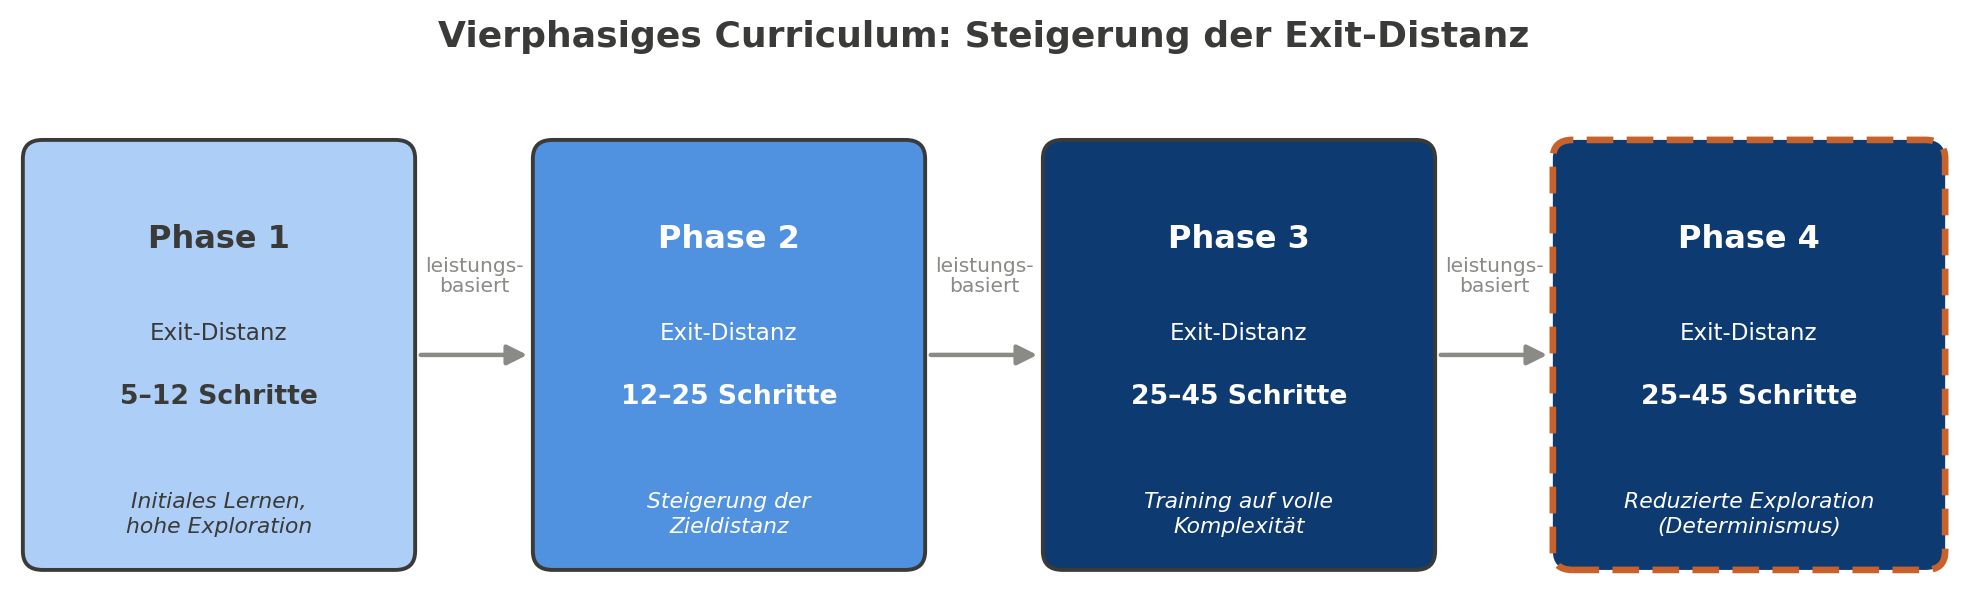
\includegraphics[width=0.85\textwidth]{Bilder/curriculum_phasen.png}
\caption{Struktur des vierphasigen Curriculum-Trainings mit Steigerung der Exit-Distanz}
\label{fig:curriculum_phasen}
\end{figure}

Wichtig für den Trainingserfolg ist, dass der Wechsel zwischen den ersten drei Phasen rein leistungsbasiert abläuft. Das bedeutet, die nächste Phase startet erst beim Erreichen einer bestimmten Erfolgsquote und nicht einfach nach einer festen Zeit. Dies macht die Steuerung deutlich stabiler.

\subsection{Definition der Baselines}
\label{sec:methodik_baselines}

Um die trainierten Modelle besser einordnen zu können, wurden drei ungelernte Baselines definiert. Sie gehören nicht zum Hauptvergleich zwischen LSTM-PPO und MLP-PPO, sondern dienen als Orientierungshilfe für die Leistung (siehe Abbildung~\ref{fig:epsilon_kompass}).

\begin{figure}[htbp]
    \centering
    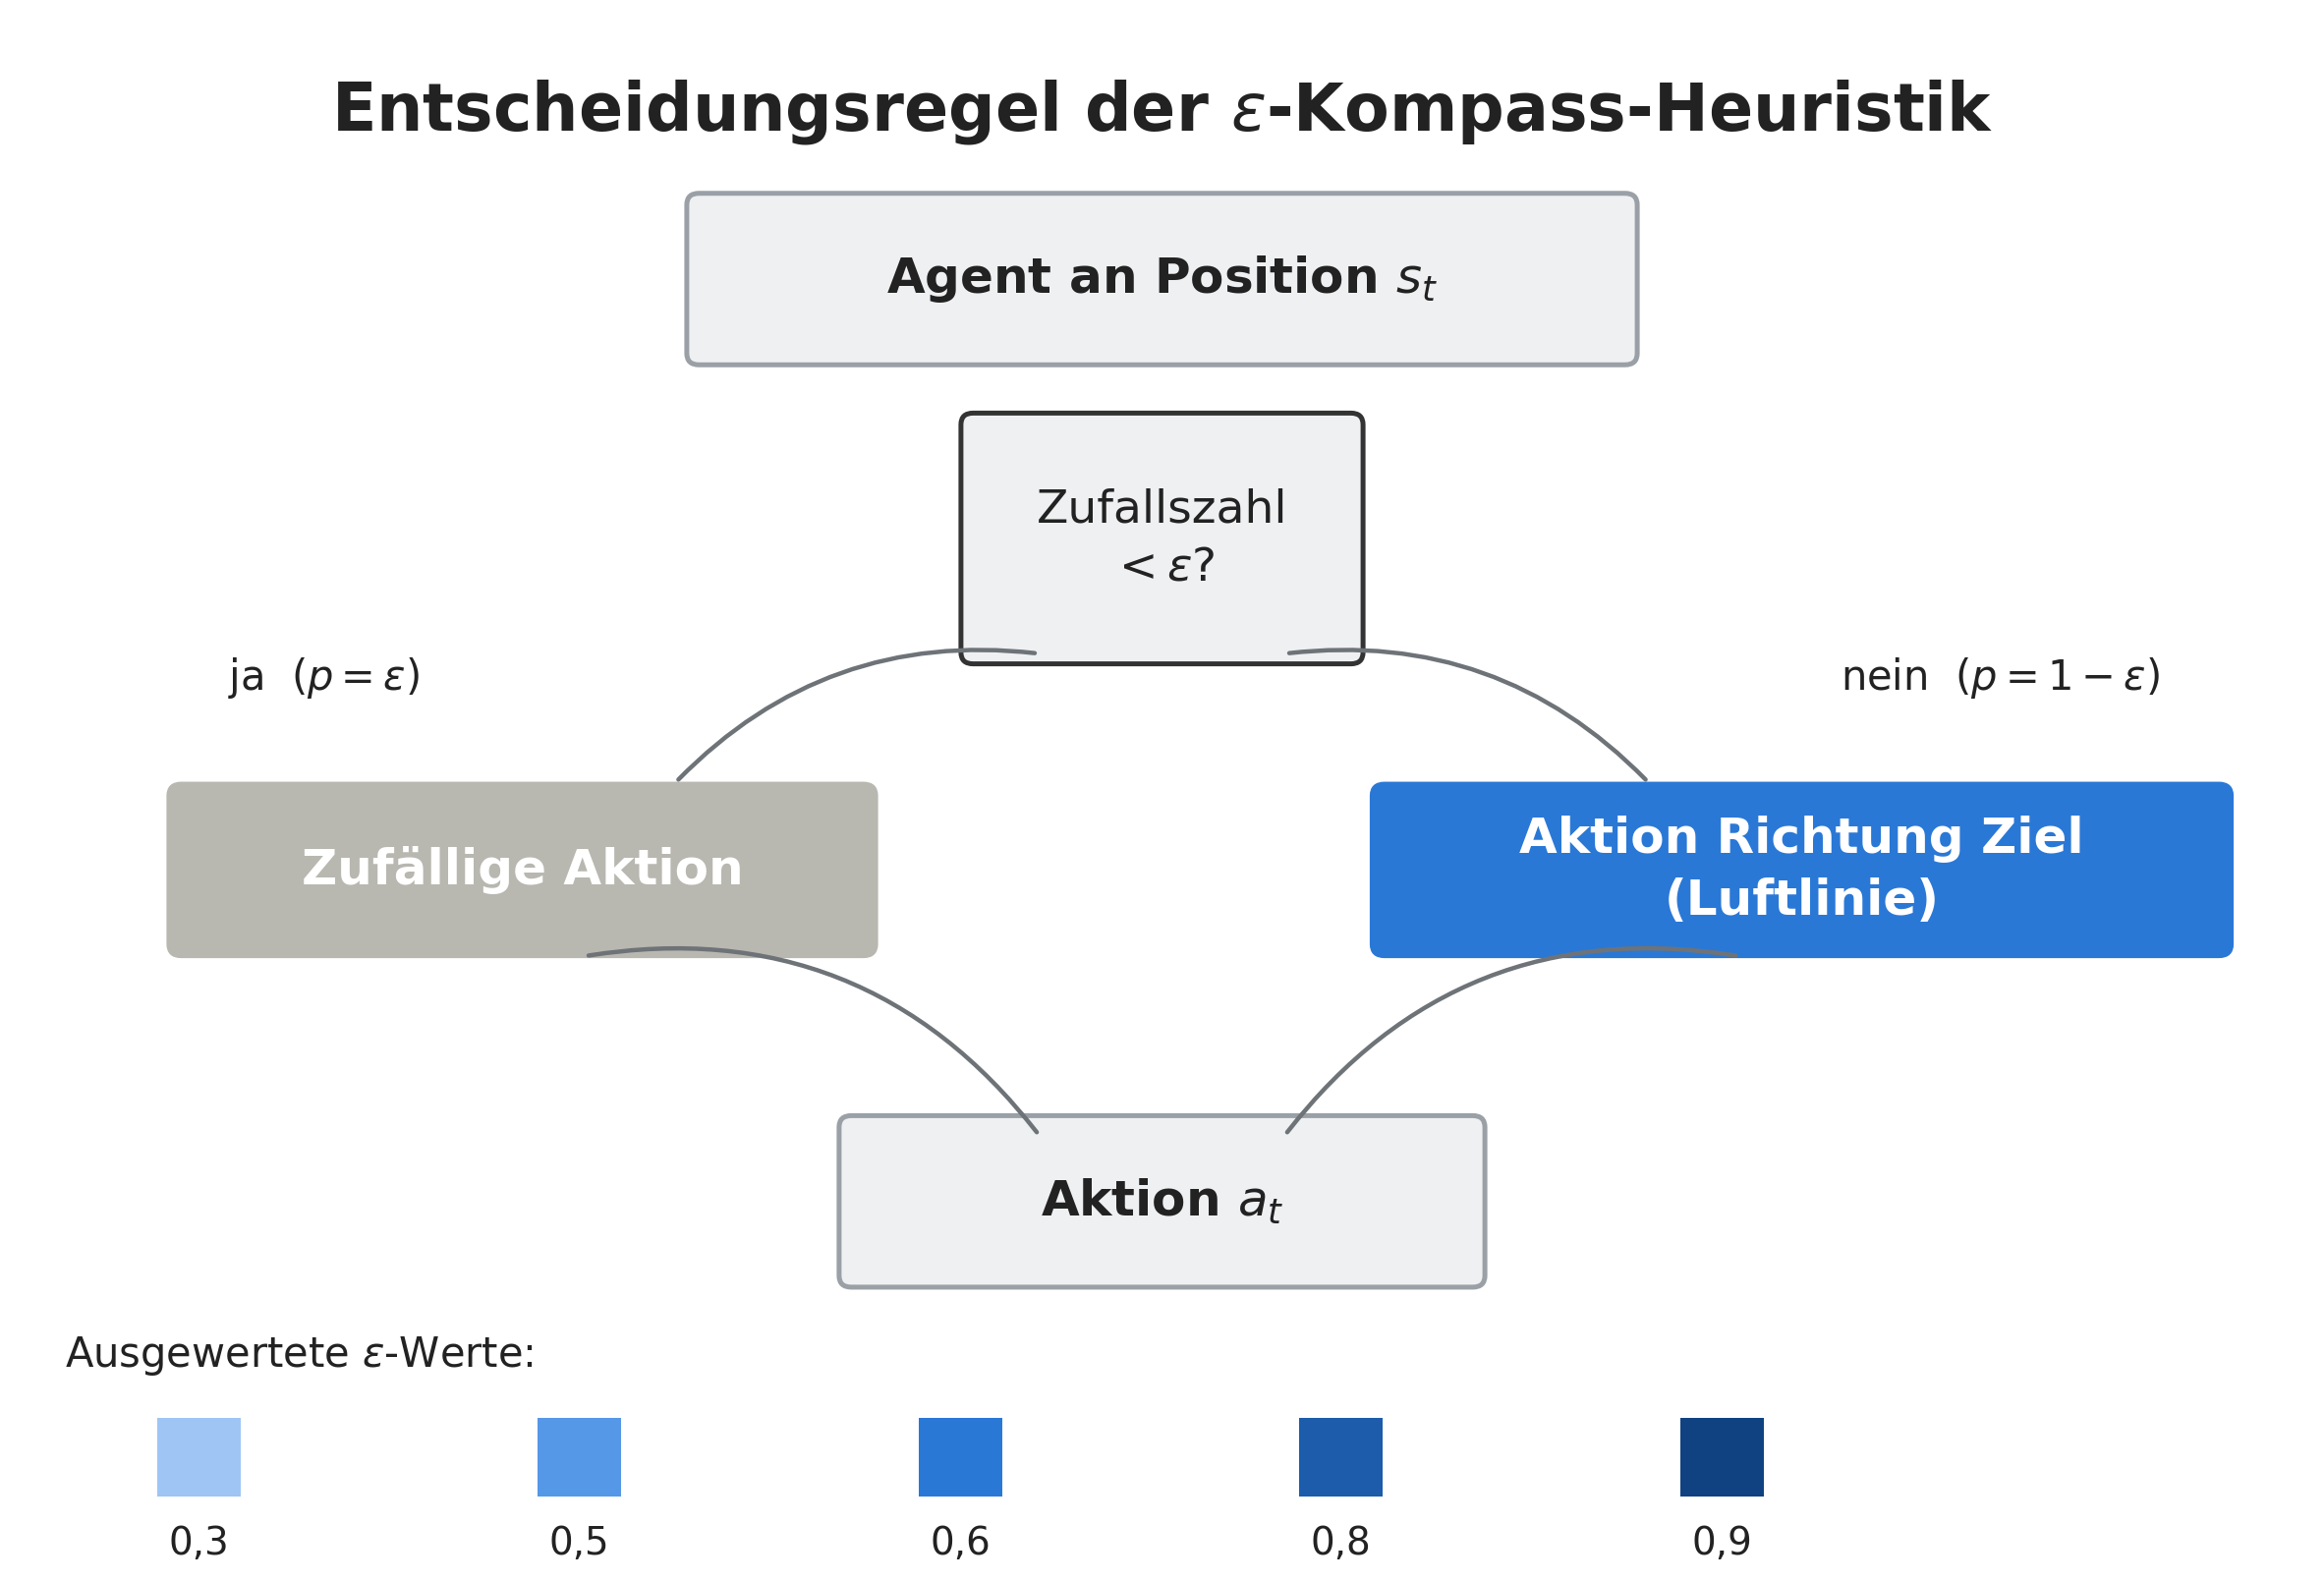
\includegraphics[width=0.85\textwidth]{Bilder/epsilon_kompass_schema.png}
    \caption{Entscheidungsregel und ausgewertete Parameter der $\varepsilon$-Kompass-Heuristik}
    \label{fig:epsilon_kompass}
\end{figure}

Das obere Limit bildet das BFS-Optimum. Dieses Orakel nutzt eine Breitensuche, um immer den mathematisch kürzesten Weg zu finden, und zeigt damit das absolute Maximum an Pfadqualität auf. Das untere Limit ist der Random-Agent, der völlig zufällige Aktionen wählt. Dazwischen liegt die $\varepsilon$-Kompass-Heuristik: Sie wählt mit einer Wahrscheinlichkeit von $\varepsilon$ einen zufälligen Schritt und bewegt sich ansonsten geradlinig in Richtung Ziel. Diese Heuristik wurde mit verschiedenen Werten getestet ($\varepsilon \in \{0{,}3; 0{,}5; 0{,}6; 0{,}8; 0{,}9\}$), um aufzuzeigen, wie Erfolgsquote und Streckenlänge in dieser Umgebung typischerweise zusammenhängen.

\subsection{Trainings- und Evaluationsprotokoll}
\label{sec:methodik_protokoll}

Um verlässliche und reproduzierbare Ergebnisse zu erhalten, wurde das Vorgehen für das Training und die Evaluation strikt festgelegt. Das Training lief über sieben unabhängige Zufalls-Seeds. Danach wurden die Modelle auf zwei komplett neuen Umgebungssets getestet, die während des Trainings nicht vorkamen: dem regulären Testset A (Seeds 7000–7049) und einem zusätzlichen Holdout-Set B (Seeds 8000–8049), um die Generalisierungsfähigkeit zu prüfen.

%TODO Schnitt 2232 Schritte woher weißt du das????
Da ein rein zufällig agierender Agent im Schnitt 2232 Schritte bis zum Ziel benötigt, war für die Tests ein festes Episodenlimit zwingend erforderlich. Ohne ein solches Limit ließe sich die Erfolgsquote nicht sinnvoll berechnen, da ein schlechter Agent sonst unendlich lange im Labyrinth verweilen würde. Überschreitet ein Agent das Limit, gilt der Versuch strikt als gescheitert. 

Zusätzlich werden die Modelle zweigleisig ausgewertet: einmal deterministisch (der Agent wählt immer die Aktion mit der höchsten Wahrscheinlichkeit) und einmal stochastisch (die Aktion wird anhand der gelernten Verteilung gesampelt). Dieser Schritt ist essenziell, um zu bewerten, ob das Netzwerk eine belastbare Richtungsstrategie verstanden hat oder lediglich durch stochastisches Raten ans Ziel gelangt.

Bei den Metriken ist die Erfolgsquote (Success Rate) das wichtigste Kriterium, gefolgt von der Pfadqualität. Der Grund dafür liegt darin, dass in ähnlichen POMDP-Benchmarks (wie Procgen, MiniGrid oder POPGym) die Erfolgsquote durchgehend als Standard gilt. Die grundsätzliche Fähigkeit, das Problem überhaupt zu lösen, wird in diesem Kontext höher gewichtet als eine perfekte Routenplanung.

\subsection{Validierungsstrategie und Umgang mit Trainingsinstabilitäten}
\label{sec:methodik_iteration}

Um einen stabilen Trainingsverlauf zu gewährleisten, musste der Prozess durchgehend überwacht und angepasst werden. Da Reinforcement Learning in solchen Umgebungen häufig dazu neigt, sich festzufahren oder den Lernprozess einzustellen, wurde gezielt auf spezifische Fehlerbilder geachtet.

Erstens half das leistungsbasierte Curriculum dabei, unkontrollierte Abstürze zu verhindern. Bei einem rein zeitbasierten Wechsel der Phasen besteht die Gefahr des sogenannten \textit{Catastrophic Forgetting}: Der Agent verlernt beim Sprung in die nächste Phase plötzlich grundlegende Fähigkeiten, und die Erfolgsquote stürzt dauerhaft auf nahezu $0\,\%$ ab.

Zweitens mussten die Parameter für die rekurrenten Netzwerke sehr genau justiert werden. Vor allem der Entropie-Koeffizient war entscheidend, damit der Agent lange genug neue Wege ausprobierte. Gleichzeitig durfte die Schrittzahl pro Update für das LSTM nicht zu hoch angesetzt werden, um das typische Problem der verschwindenden Gradienten (Vanishing Gradient) zu umgehen. Ohne diese Anpassungen bleibt das Training oft komplett stehen oder der Agent zeigt einen \textit{Mode Collapse} – dreht sich also beispielsweise nur noch auf der Stelle.

Drittens erwies sich die Puffergröße für das Reward Shaping als kritischer Faktor. Der Ringpuffer musste groß genug dimensioniert werden, damit der Agent nicht fälschlicherweise für Rückwärtsschritte belohnt wird. Ein zu klein gewählter Puffer führte häufig zum \textit{Reward Hacking}: Der Agent pendelte nur noch zwischen zwei Feldern hin und her, um dauerhaft kleine Belohnungen zu sammeln, anstatt den Ausgang anzusteuern. 

Um diese Risiken systematisch im Blick zu behalten, wurde der Trainingsprozess anhand der Indikatoren aus Tabelle~\ref{tab:troubleshooting} überwacht und entsprechend korrigiert.

\begin{table}[htbp]
    \centering
    \caption{Diagnose- und Interventionsmatrix der aufgetretenen Trainingsinstabilitäten}
    \label{tab:troubleshooting}
    \begin{tabular}{p{4.2cm} p{5cm} p{5.3cm}}
        \toprule
        \textbf{Symptom / Fehlerbild} & \textbf{Indikator in den Metriken} & \textbf{Angewandte Interventionsstrategie} \\
        \midrule
        \textbf{Catastrophic Forgetting} \newline (Abrupter Leistungsabfall) & Erfolgsquote stürzt beim Phasenwechsel drastisch ab und erholt sich nicht. & Strikte Schwellenwerte für den Wechsel eingeführt (erst ab konstanten $85\,\%$ Erfolg über ein gleitendes Fenster). \\[2ex]

        \textbf{Lernstillstand / \newline Mode Collapse} \newline (Zwanghaftes Kreiseln) & Aktions-Entropie fällt schlagartig ab; Agent erreicht stets das Episodenlimit. & Entropie-Koeffizienten erhöht; Schrittzahl pro Update für das LSTM limitiert und angepasst. \\[2ex]

        \textbf{Reward Hacking} \newline (Pendeln zwischen Zellen) & Steigender Episoden-Reward bei stagnierender oder sinkender Erfolgsquote. & Ringpuffer deutlich vergrößert; Potenzialfunktion auf mathematische Korrektheit geprüft. \\
        \bottomrule
    \end{tabular}
\end{table}

%%%%%%%%%%%%%%%%%%%%%%%%%%%%%%%%%%%%%%%%%%%%%%%%%%%%%%%%%%%%%%%%
% BEGIN: kapitel/04_implementierung.tex
%%%%%%%%%%%%%%%%%%%%%%%%%%%%%%%%%%%%%%%%%%%%%%%%%%%%%%%%%%%%%%%%
\chapter{Umsetzung und technische Realisierung}
\label{chap:umsetzung}

Dieses Kapitel beschreibt die praktische Implementierung des im vorherigen Kapitel vorgestellten Konzepts zur prozeduralen Weltengenerierung. Die Realisierung erfolgt in der Programmiersprache C++ innerhalb der Kernkomponente \texttt{world.cpp}. Das Hauptziel der Implementierung besteht darin, eine performante, deterministische und speichereffiziente Erzeugung von Welt-Chunks zur Laufzeit zu gewährleisten.

Dazu werden nachfolgend die zentralen Softwarebausteine – von der mathematischen Rauscherzeugung über die biomspezifische Zuweisung bis hin zu den topologischen Sicherheits- und Pfad-Algorithmen – anhand relevanter Quellcode-Ausschnitte und deren Datenstrukturen detailliert erläutert.

\section{Implementierung der Weltgenerierung}

\subsection{Implementierung der Rauscherzeugung und des Koordinaten-Hashings}
\label{sec:umsetzung_noise}

Das Fundament der deterministischen Landschaftserzeugung bildet ein zweistufiger Prozess: Zunächst werden diskrete Raumkoordinaten deterministisch in Pseudozufallswerte transformiert, welche anschließend durch ein bilineares Value-Noise-Verfahren kontinuierlich interpoliert werden (siehe Kapitel~3.1.1).

\subsubsection{Deterministischer Hash-Mixer}
Um ohne aufwändige Speicherzustände für beliebige Weltkoordinaten $(x, y)$ reproduzierbare Zufallswerte zu erhalten, nutzt das System einen 64-Bit-Hash-Mixer. Listing~\ref{lst:hash_mixer} zeigt die konkrete Umsetzung der Abbildung von Raumkoordinaten auf das normierte Intervall $[0, 1)$.

\begin{lstlisting}[language=C++, caption={Verwendung des 64-Bit SplitMix-Mixers und Value-Noise-Interpolation in \texttt{world.cpp}}, label={lst:hash_mixer}]
std::uint64_t World::mix(std::uint64_t value) const {
    value ^= value >> 30;
    value *= 0xbf58476d1ce4e5b9ULL;
    value ^= value >> 27;
    value *= 0x94d049bb133111ebULL;
    value ^= value >> 31;
    return value;
}

double World::noise01(int worldX, int worldY, std::uint64_t salt) const {
    std::uint64_t value = static_cast<std::uint64_t>(worldX) * 0x9e3779b185ebca87ULL;
    value ^= static_cast<std::uint64_t>(worldY) * 0xc2b2ae3d27d4eb4fULL;
    value ^= seed_ * 0x165667b19e3779f9ULL;
    value ^= salt;
    value = mix(value);

    constexpr double kScale = 1.0 / static_cast<double>(0xFFFFFFFFFFFFULL);
    return static_cast<double>(value & 0xFFFFFFFFFFFFULL) * kScale;
}

auto sampleValue = [&](double x, double y, std::uint64_t salt) {
    const int x0 = static_cast<int>(std::floor(x));
    const int y0 = static_cast<int>(std::floor(y));
    const int x1 = x0 + 1;
    const int y1 = y0 + 1;
    const double tx = smoothstep(x - static_cast<double>(x0));
    const double ty = smoothstep(y - static_cast<double>(y0));

    const double v00 = noise01(x0, y0, salt);
    const double v10 = noise01(x1, y0, salt);
    const double v01 = noise01(x0, y1, salt);
    const double v11 = noise01(x1, y1, salt);
    return lerp(lerp(v00, v10, tx), lerp(v01, v11, tx), ty);
};
\end{lstlisting}

\subsubsection{Variablen und Datenstrukturen}
Die in Listing~\ref{lst:hash_mixer} gezeigten Funktionen bilden die mathematische Basis für die rasterfreie Weltengenerierung:

\begin{itemize}
    \item \texttt{mix}: Eine Implementierung der 64-Bit-SplitMix-Pseudozufallsfunktion. Sie nutzt Bit-Shifting und Multiplikationen mit großen Primzahl-Konstanten, um Bit-Korrelationen zu zerstören und eine gleichmäßige Verteilung zu garantieren.
    \item \texttt{worldX}, \texttt{worldY}: Die diskreten Ganzzahlkoordinaten des abzufragenden Raumpunktes auf dem Weltgitter.
    \item \texttt{seed\_}: Die Instanzvariable des globalen Welt-Seeds. Sie stellt sicher, dass dieselben Raumkoordinaten bei identischem Seed exakt reproduzierbare Ergebnisse liefern.
    \item \texttt{salt}: Ein variabler 64-Bit-Wert, der als Salt dient. Er verhindert, dass unterschiedliche Generierungsebenen (z.\,B. Dichte, Erz- und Baumpopulation) auf derselben Koordinate synchrone Muster aufweisen.
    \item \texttt{kScale}: Ein präziser Skalierungsfaktor ($\frac{1}{2^{48}-1}$), der die untersten 48 Bit des Bitmusters über eine Bitmaskierung (\texttt{0xFFFFFFFFFFFFULL}) exakt auf das normierte Intervall $[0, 1]$ abbildet.
    \item \texttt{x0, y0, x1, y1}: Ganzzahlige Eckpunkte der Gitterzelle, in der der kontinuierliche Punkt $(x, y)$ liegt.
    \item \texttt{tx, ty}: Die mittels \texttt{smoothstep} transformierten relativen Abstände innerhalb der Zelle, welche als Interpolationsgewichte dienen.
    \item \texttt{v00, v10, v01, v11}: Die an den vier Gitterecken über \texttt{noise01} determinierten Zufallswerte, welche abschließend mittels zweifacher linearer Interpolation (\texttt{lerp}) verschmolzen werden.
\end{itemize}

\subsection{Biomeinteilung und Objekt-Placement}
\label{sec:umsetzung_biome}

Nach der Bereitstellung der kontinuierlichen Rauschfunktionen erfolgt die Zuweisung konkreter Kacheltypen (\texttt{TileType}) zu den Raumkoordinaten $(x, y)$. Die Funktion \texttt{sampleBaseTile} steuert diesen Prozess in Abhängigkeit vom übergeordneten Chunk-Biom und biomspezifischen Schwellenwerten (\textit{Thresholds}).

\subsubsection{Implementierung der Kachelauswertung}
In Listing~\ref{lst:sample_base_tile} ist die Realisierung der \texttt{sampleBaseTile}-Methode dargestellt. Sie bestimmt zunächst über das Chunk-Raster (\texttt{floorDiv}) das zugrundeliegende Biom (\texttt{biomeTag}) und wertet anschließend drei unabhängige Noise-Layer (Dichte, Erzvorkommen, Baumdichte) aus.

\begin{lstlisting}[language=C++, caption={Biom-Tagging und Schwellenwertauswertung in \texttt{world.cpp}}, label={lst:sample_base_tile}]
TileType World::sampleBaseTile(int worldX, int worldY, const WorldGenConfig& cfg) const {
    const int cx = floorDiv(worldX, kChunkSize);
    const int cy = floorDiv(worldY, kChunkSize);
    const int biomeTag = biomeTagForChunk(cx, cy);

    const double density = noise01(worldX, worldY, cfg.densitySalt);
    const double ore = noise01(worldX, worldY, cfg.oreSalt);
    const double trees = noise01(worldX, worldY, cfg.treeSalt);

    double wallThreshold = 0.11;
    double oreThreshold = 0.03;
    double treeThreshold = 0.08;

    // Biomspezifische Schwellenwert-Profile
    switch(biomeTag) {
        case 0:  // Grasland: WENIGER BAEUME
            wallThreshold = 0.10; oreThreshold = 0.03; treeThreshold = 0.05; break;
        case 1:  // Wald: VIELE BAEUME, WENIG STEINE
            wallThreshold = 0.07; oreThreshold = 0.015; treeThreshold = 0.23; break;
        case 2:  // Wueste: VIELE STEINE, KEINE BAEUME
            wallThreshold = 0.19; oreThreshold = 0.08; treeThreshold = 0.0; break;
        case 3:  // Bergland: VIELE STEINE UND ERZE
            wallThreshold = 0.25; oreThreshold = 0.10; treeThreshold = 0.02; break;
        case 4:  // Steppe: GRASLAND MIT ETWAS MEHR BAEUMEN
            wallThreshold = 0.11; oreThreshold = 0.03; treeThreshold = 0.09; break;
        case 5:  // Tundra: NORMALE STEINE UND BAEUME
            wallThreshold = 0.14; oreThreshold = 0.05; treeThreshold = 0.07; break;
        case 6:  // Hoelle: HOHE WAND- UND ERZDICHTE
            wallThreshold = 0.23; oreThreshold = 0.09; treeThreshold = 0.06; break;
        default: break;
    }

    TileType tile = TileType::Empty;

    // Gewaessermaske besitzt hoechste Prioritaet (Freiraum)
    if(lakeMaskAt(worldX, worldY)) {
        return TileType::Empty;
    }

    // Auswertung der Objektgrenzwerte
    if(density < wallThreshold) {
        tile = TileType::Wall;
    }
    // Erzvorkommen exklusiv im Bergland (Biom 3)
    if(biomeTag == 3 && ore < oreThreshold) {
        tile = TileType::Resource;
    }
    // Baumpopulation auf verbleibenden Freiflaechen
    if(treeThreshold > 0.0 && tile == TileType::Empty && trees < treeThreshold) {
        tile = TileType::Tree;
    }

    return tile;
}
\end{lstlisting}

\subsubsection{Logik und Priorisierung der Kachelzuweisung}
Die Auswertung in Listing~\ref{lst:sample_base_tile} folgt einer strikten Prioritätenhierarchie, um ungewollte Überschreibungen von Spielelementen zu vermeiden:

\begin{enumerate}
    \item \textbf{Chunk-Rasterung (\texttt{floorDiv}):} Raumkoordinaten werden zunächst in diskrete Chunk-Koordinaten $(cx, cy)$ transformiert, um das für den gesamten Chunk gültige Biom (\texttt{biomeTag} $\in [0, 6]$) abzufragen.
    \item \textbf{Drei unabhängige Noise-Layer:} Durch die Übergabe unterschiedlicher Salt-Werte (\texttt{cfg.densitySalt}, \texttt{cfg.oreSalt}, \texttt{cfg.treeSalt}) an die Funktion \texttt{noise01} werden räumlich entkoppelte Zufallswerte für Wand-, Erz- und Baumvorkommen generiert.
    \item \textbf{Biomspezifische Profile (\texttt{switch}):} Das ermittelte \texttt{biomeTag} überschreibt die Standard-Schwellenwerte für Wand-, Erz- und Baumdichte. So erzwingt Biom 2 (Wüste) beispielsweise eine Baumgrenze von \texttt{treeThreshold = 0.0} (kein Baumbewuchs), während Biom 1 (Wald) mit \texttt{treeThreshold = 0.23} eine hohe Baumdichte aufweist.
    \item \textbf{Gewässermaske (\texttt{lakeMaskAt}):} Seen fungieren als hindernisfreie Areale. Gibt \texttt{lakeMaskAt} den Wert \texttt{true} zurück, bricht die Funktion sofort ab und gibt \texttt{TileType::Empty} zurück.
    \item \textbf{Hierarchische Klassifizierung:}
    \begin{itemize}
        \item Unterschreitet die Dichte den Schwellenwert \texttt{wallThreshold}, wird das Tile primär als Wandoberfläche (\texttt{TileType::Wall}) definiert.
        \item Erze (\texttt{TileType::Resource}) werden exklusiv im Bergland (\texttt{biomeTag == 3}) platziert, sofern der Erz-Noise-Wert unter \texttt{oreThreshold} liegt.
        \item Bäume (\texttt{TileType::Tree}) spritzen ausschließlich auf bisher unbesetzten Feldern (\texttt{tile == TileType::Empty}) unter Berücksichtigung von \texttt{treeThreshold}.
    \end{itemize}
\end{enumerate}

\subsection{Topologische Sicherheits-Fallbacks und Spawn-Freiräume}
\label{sec:umsetzung_pathing}

Um unabhängig von den pseudozufälligen Rauschwerten und den gewählten Biomschwellenwerten eine unbedingte Spielbarkeit (\textit{Playability}) zu garantieren, implementiert das System deterministische Sicherheits-Fallbacks. Diese stellen sicher, dass der Spieler weder in unpassierbaren Hindernissen startet noch ein unlösbares Level vorfindet.

\subsubsection{Implementierung des Manhattan-Carvers und der Freiradien}
In Listing~\ref{lst:manhattan_carver} ist der relevante Ausschnitt aus der Methodenreihenfolge in \texttt{reset()} sowie die vollständige Implementierung der Methode \texttt{carveGuaranteedPath} dargestellt, deren methodischer Entwurf bereits vorgestellt wurde (siehe Kapitel~3.1.2).

\begin{lstlisting}[language=C++, caption={Freiradien-Erzeugung und Manhattan-Path-Carver in \texttt{world.cpp}}, label={lst:manhattan_carver}]
// Ausschnitt aus World::reset()
for(int dy = -cfg.spawnClearRadius; dy <= cfg.spawnClearRadius; ++dy) {
    for(int dx = -cfg.spawnClearRadius; dx <= cfg.spawnClearRadius; ++dx) {
        setTile(spawn_.x + dx, spawn_.y + dy, TileType::Empty);
    }
}

if(cfg.forceGuaranteedPath) {
    carveGuaranteedPath();
}

for(int dy = -cfg.exitClearRadius; dy <= cfg.exitClearRadius; ++dy) {
    for(int dx = -cfg.exitClearRadius; dx <= cfg.exitClearRadius; ++dx) {
        setTile(exit_.x + dx, exit_.y + dy, TileType::Empty);
    }
}
setTile(exit_.x, exit_.y, TileType::Exit);

// Deterministische Manhattan-Pfadgenerierung
void World::carveGuaranteedPath() {
    const auto& cfg = gameConfig().world;
    int x = spawn_.x;
    int y = spawn_.y;

    setTile(x, y, TileType::Empty);

    // 1. Horizontale Trassierung (X-Achse)
    while(x != exit_.x) {
        x += (x < exit_.x) ? 1 : -1;
        setTile(x, y, TileType::Empty);
    }

    // 2. Vertikale Trassierung (Y-Achse)
    while(y != exit_.y) {
        y += (y < exit_.y) ? 1 : -1;
        setTile(x, y, TileType::Empty);
    }

    // Erneute Durchsetzung der Freiradien nach dem Carving
    for(int dy = -cfg.spawnClearRadius; dy <= cfg.spawnClearRadius; ++dy) {
        for(int dx = -cfg.spawnClearRadius; dx <= cfg.spawnClearRadius; ++dx) {
            setTile(spawn_.x + dx, spawn_.y + dy, TileType::Empty);
        }
    }

    for(int dy = -cfg.exitClearRadius; dy <= cfg.exitClearRadius; ++dy) {
        for(int dx = -cfg.exitClearRadius; dx <= cfg.exitClearRadius; ++dx) {
            setTile(exit_.x + dx, exit_.y + dy, TileType::Empty);
        }
    }

    setTile(exit_.x, exit_.y, TileType::Exit);
}
\end{lstlisting}

\subsubsection{Funktionsweise und Ausführungsreihenfolge}
Die in Listing~\ref{lst:manhattan_carver} gezeigte Pfadsicherung folgt einem klaren, mehrstufigen Ablauf:

\begin{enumerate}
    \item \textbf{Freiradienen-Erzeugung (Quadratischer Bereich):} Sowohl um die Spawn-Koordinate \texttt{spawn\_} als auch um die Exit-Koordinate \texttt{exit\_} wird über verschachtelte Schleifen ein quadratischer Radius der Größe \texttt{cfg.spawnClearRadius} bzw. \texttt{cfg.exitClearRadius} vollständig freigeräumt (\texttt{TileType::Empty}). Dies stellt sicher, dass der Spieler ohne Kollisionsprobleme starten kann.
    \item \textbf{Schalterbasierte Pfadfreischaltung (\texttt{forceGuaranteedPath}):} Die Pfadgenerierung wird rein konfigurationsbasiert über das Flag \texttt{cfg.forceGuaranteedPath} gesteuert (welches laut \texttt{game\_config.json} standardmäßig aktiviert ist).
    \item \textbf{Orthogonale Manhattan-Trassierung:} Die Funktion \texttt{carveGuaranteedPath} startet am Punkt \texttt{spawn\_} und schlägt schrittweise einen absolut freien Korridor in die Umgebung. Die Abfolge ist fest auf die Orthogonalen festgelegt:
    \begin{itemize}
        \item Zunächst wird der $x$-Wert der aktuellen Position schrittweise an \texttt{exit\_.x} angeglichen und dabei jede betroffene Zelle auf \texttt{TileType::Empty} gesetzt.
        \item Anschließend erfolgt die vertikale Anpassung der $y$-Position, bis die Koordinaten von \texttt{exit\_} erreicht sind.
    \end{itemize}
    \item \textbf{Redundante Sicherung des Exits:} Nach dem Durchschneiden des Pfades werden die Freiradien um den Spawn- und Exit-Bereich erneut freigeräumt und das Zielfeld explizit mit \texttt{TileType::Exit} markiert, damit der Level-Ausgang nicht versehentlich überschrieben wird.
\end{enumerate}

\subsection{Generierung von Gewässern und dynamische Strand-Derivation}
\label{sec:umsetzung_lakes_beaches}

Die Erzeugung von Seen und deren optischer Übergangszone (Strände) erfordert eine Entkopplung der logischen Weltrepräsentation von der visuellen Darstellung. Während Gewässer als harte Kollisions- bzw. Freiräume im Weltmodell definiert sind, entstehen Strände dynamisch über Nachbarschaftsauswertungen im Render-Pfad.

\subsubsection{Mathematische Seen-Maskierung (\texttt{lakeMaskAt})}
Gewässer dürfen im Gegensatz zu einzelnen Bäumen oder Hindernissen nicht als vereinzelte Pixel-Fehler erscheinen, sondern müssen als zusammenhängende, organische Binnengewässer im Terrain hervortreten. Dazu verwendet die Funktion \texttt{lakeMaskAt} in \texttt{world.cpp} niederfrequentes Rauschen (\textit{Low-Frequency Noise}).

\begin{lstlisting}[language=C++, caption={Low-Frequency-Value-Noise für zusammenhängende Gewässermasken in \texttt{world.cpp}}, label={lst:lake_mask}]
bool World::lakeMaskAt(int worldX, int worldY) const {
    const auto& cfg = gameConfig().world;
    if (!cfg.enableLakes) {
        return false;
    }

    // Niederfrequente Skalierung für flächige Strukturen
    const double n1 = sampleValueNoise(
        static_cast<double>(worldX) * 0.035, 
        static_cast<double>(worldY) * 0.035, 
        cfg.lakeSalt
    );
    const double n2 = sampleValueNoise(
        static_cast<double>(worldX) * 0.018 + 100.0, 
        static_cast<double>(worldY) * 0.018 - 50.0, 
        cfg.lakeSalt + 100
    );

    // Mischen beider Rauschschichten
    const double lakeScore = n1 * 0.6 + n2 * 0.4;

    // Schwellenwertentscheidung fuer seltene, koharente Seen
    return lakeScore > 0.86;
}

bool World::isLakeAt(int worldX, int worldY) const {
    // Spawn- und Exit-Zonen dürfen niemals von Seen überdeckt werden
    if ((worldX == spawn_.x && worldY == spawn_.y) || 
        (worldX == exit_.x && worldY == exit_.y)) {
        return false;
    }
    return lakeMaskAt(worldX, worldY);
}
\end{lstlisting}

Wie in Listing~\ref{lst:lake_mask} gezeigt, nutzt die Berechnung zwei transformierte Noise-Funktionen mit kleinen Frequenzfaktoren ($0{,}035$ und $0{,}018$). Durch die gewichtete Kombination beider Schichten (\texttt{lakeScore}) und die Wahl eines hohen Schwellenwerts ($> 0{,}86$) entstehen großflächige, organisch geformte Seenstrukturen („blobs“). Die Hilfsfunktion \texttt{isLakeAt} stellt zudem sicher, dass kritische Positionen wie der Spawn- und der Exit-Punkt niemals durch Gewässer blockiert werden.

\subsubsection{Prozedurale Strand-Derivation im Renderer}
Anstatt Sand/Strand als eigenständige Kacheltypen (\texttt{TileType}) im Speicher zu verwalten, wird die Strandzone zur Laufzeit im Render-Pfad (\texttt{render\_engine.cpp}) anhand einer $3 \times 3$-Nachbarschaftsanalyse abgeleitet.

\begin{lstlisting}[language=C++, caption={Nachbarschaftsbasierte Stranddarstellung im Render-Pfad in \texttt{render\_engine.cpp}}, label={lst:beach_rendering}]
bool RenderEngine::lakeOrAdjacentAt(int worldX, int worldY) const {
    // Überprüfung der 3x3-Nachbarschaft auf angrenzende Seen
    for (int dy = -1; dy <= 1; ++dy) {
        for (int dx = -1; dx <= 1; ++dx) {
            if (world_.isLakeAt(worldX + dx, worldY + dy)) {
                return true;
            }
        }
    }
    return false;
}

// Auszug aus der Tile-Rendering-Schleife:
if (world_.isLakeAt(x, y)) {
    drawWaterTile(x, y);
} else if (lakeOrAdjacentAt(x, y) && isPassable(x, y)) {
    drawSandSpriteOverlay(x, y); // Strand-Overlay für See-Nachbarn
    drawBaseTile(x, y);
} else {
    drawBaseTile(x, y);
}
\end{lstlisting}

\begin{itemize}
    \item \textbf{Effizienz durch Zustandslosigkeit:} Durch die Trennung von Weltlogik und Darstellung spart die Weltengenerierung Speicherplatz, da keine eigenen Sand-Kacheln in der Chunk-Datenstruktur abgelegt werden müssen.
    \item \textbf{Konditionale Überlagerung:} Die Funktion \texttt{lakeOrAdjacentAt} prüft, ob sich im direkten $3 \times 3$-Umfeld ein Gewässer befindet. Ist dies der Fall und handelt es sich nicht um eine blockierte Kachel (z.\,B. Wand oder Baum), rendert die Engine dynamisch ein Sand-Overlay unter dem Basis-Boden.
\end{itemize}

\begin{figure}[htbp]
    \centering
    
\includegraphics[height=6cm]{Bilder/lakes.PNG}
    \caption{Nahaufnahme einer prozedural generierten Seenstruktur mit organischer, rauschbasierter Uferlinie und dynamisch abgeleitetem Strand-Overlay an den Begehbarkeitsgrenzen. Quelle: Eigene Darstellung (Screenshot des Prototyps).}
    \label{fig:lake_detail}
\end{figure}

\subsection{Chunk-Speicherarchitektur und prozedurales Biome-Blending}
\label{sec:umsetzung_chunks_blending}

Um speicherhungrige Vorberechnungen großer Welten zu vermeiden, nutzt das System eine bedarfsgesteuerte Chunk-Verwaltung (\textit{Lazy Generation}) gekoppelt mit einer räumlich kontinuierlichen Biom-Farb- und Textursynthese im Render-Pfad.

\subsubsection{Bedarfsgesteuerte Chunk-Datenstruktur (\texttt{Lazy Generation})}
Die Weltkarte ist in quadratische Chunks der festen Kantenlänge $kChunkSize = 8$ (insgesamt 64 Tiles pro Chunk) unterteilt. Anstatt gesamte Welten beim Start im RAM abzulegen, erzeugt die Engine Chunks erst bei der ersten konkreten Zelle- oder Adressabfrage.

\begin{lstlisting}[language=C++, caption={Chunk-Speicherstruktur und Lazy-Loading-Mechanismus in \texttt{world.hpp} und \texttt{world.cpp}}, label={lst:chunk_structure}]
// Definition der kompakten Chunk-Struktur (world.hpp)
constexpr int kChunkSize = 8;

struct Chunk {
    int cx = 0;
    int cy = 0;
    bool generated = false;
    std::array<TileType, kChunkSize * kChunkSize> tiles;
};

// Effiziente Hash-Schlüssel-Generierung für Chunk-Koordinaten
inline uint64_t chunkKey(int cx, int cy) {
    return (static_cast<uint64_t>(cx) & 0xFFFFFFFFULL) | 
          ((static_cast<uint64_t>(cy) & 0xFFFFFFFFULL) << 32);
}

// Bedarfsgesteuertes Erzeugen von Chunks (world.cpp)
Chunk& World::ensureChunk(int cx, int cy) {
    const uint64_t key = chunkKey(cx, cy);
    auto it = chunks_.find(key);
    if (it != chunks_.end()) {
        return it->second;
    }

    // Chunk neu anlegen und initialisieren
    Chunk& chunk = chunks_[key];
    chunk.cx = cx;
    chunk.cy = cy;
    generateChunkTiles(chunk);
    chunk.generated = true;
    return chunk;
}
\end{lstlisting}

Wie in Listing~\ref{lst:chunk_structure} zu sehen ist, speichert die Klasse \texttt{World} alle aktiven Abschnitte in einer \texttt{std::unordered\_map<uint64\_t, Chunk>}. Der 64-Bit-Schlüssel wird bitweise aus den 32-Bit-Signed-Chunk-Koordinaten $(cx, cy)$ zusammengesetzt. Wird über \texttt{tileAt()} oder \texttt{setTile()} auf ungeneriertes Terrain zugegriffen, erzeugt \texttt{ensureChunk()} den Ziel-Chunk instantan und kapselt die Generierungslogik. Ein Aufruf von \texttt{reset()} leert die Map mittels \texttt{chunks\_.clear()}, um den Speicher vollständig freizugeben.

\begin{figure}[htbp]
    \centering
    \begin{subfigure}[b]{0.45\textwidth}
        \centering
        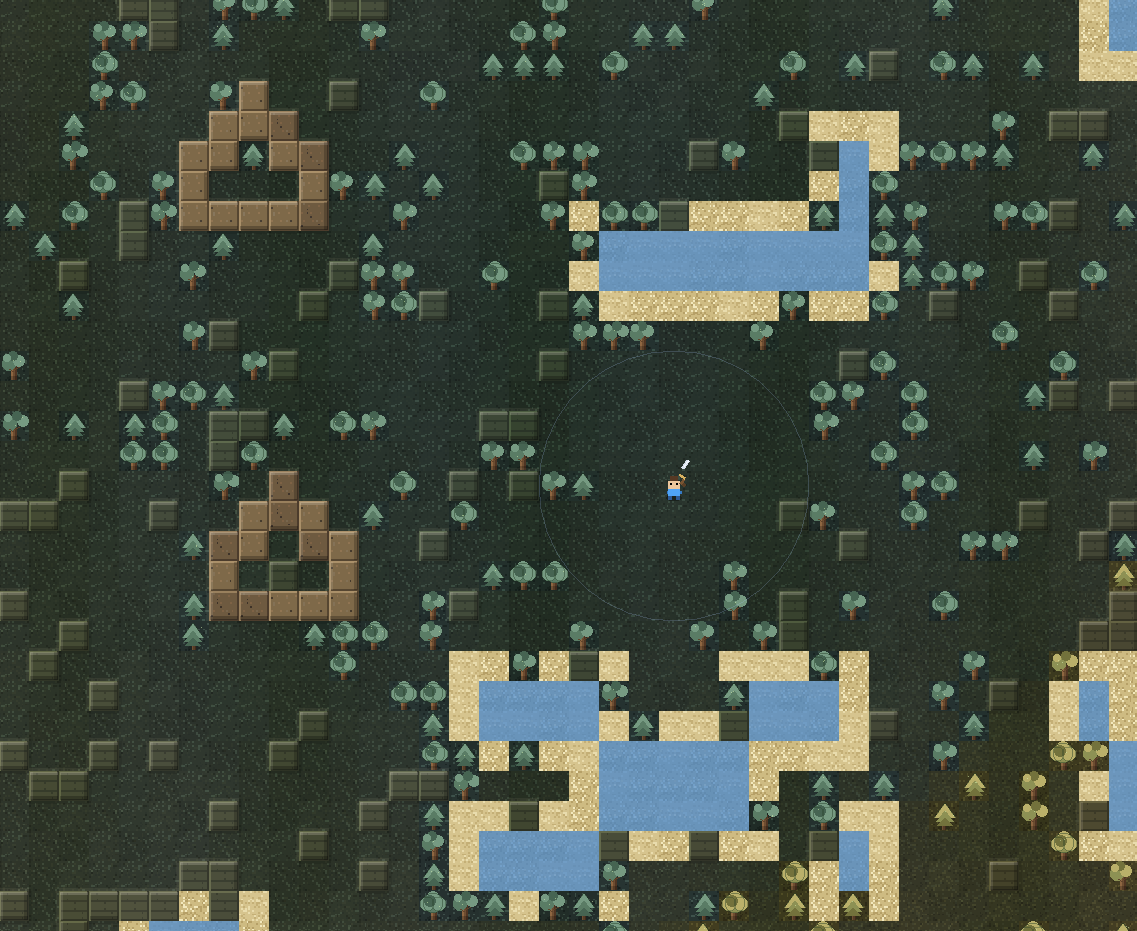
\includegraphics[height=5.5cm]{Bilder/forest biome.PNG}
        \caption{Wald-Biom: hohe Baumdichte, geringe Wandhäufigkeit.}
    \end{subfigure}
    \hfill
    \begin{subfigure}[b]{0.45\textwidth}
        \centering
        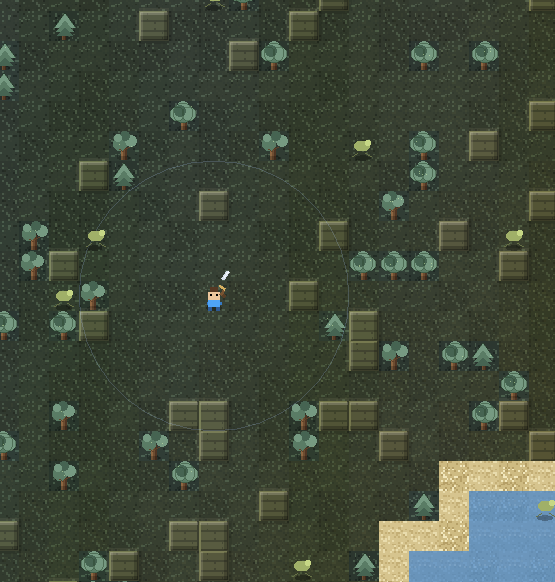
\includegraphics[height=5.5cm]{Bilder/steppe.PNG}
        \caption{Steppen-Biom: grasland-ähnlich mit leicht erhöhter Baumverteilung.}
    \end{subfigure}

    \vspace{0.3cm}

    \begin{subfigure}[b]{0.45\textwidth}
        \centering
        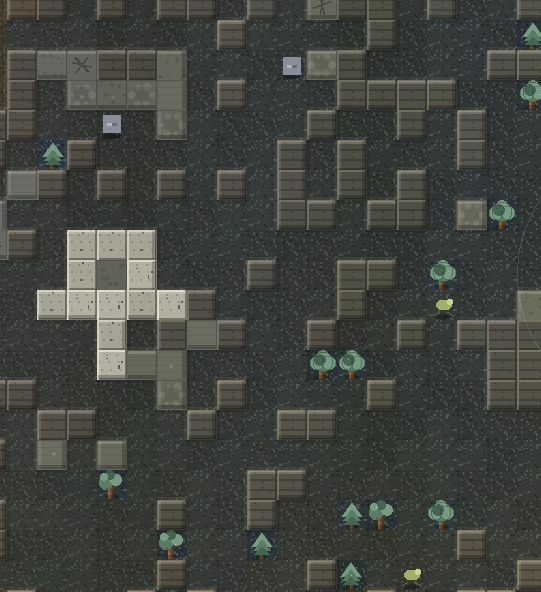
\includegraphics[height=5.5cm]{Bilder/mountain biome.PNG}
        \caption{Bergland-Biom: hohe Wand- und Erzdichte.}
    \end{subfigure}
    \hfill
    \begin{subfigure}[b]{0.45\textwidth}
        \centering
        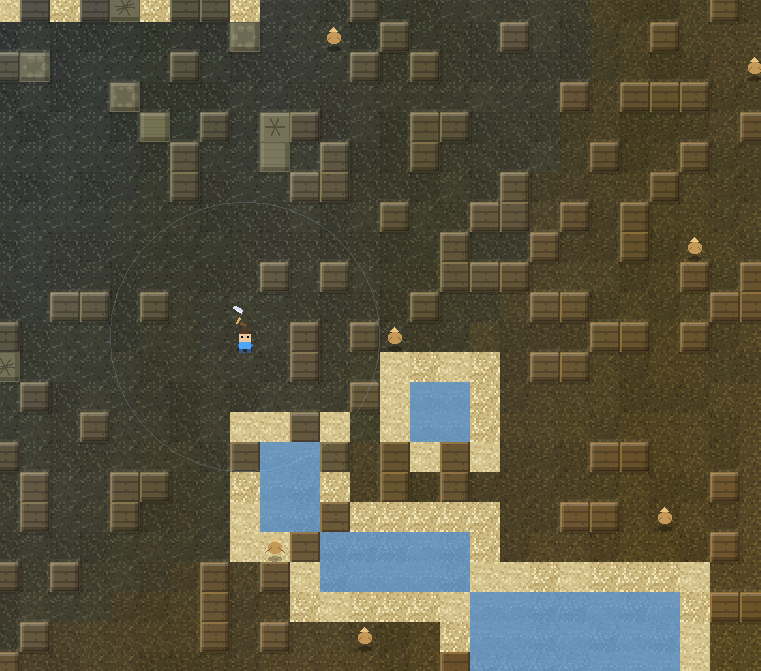
\includegraphics[height=5.5cm]{Bilder/biome desert.PNG}
        \caption{Wüsten-Biom: baumfrei, erhöhte Steindichte.}
    \end{subfigure}
    \caption{Vergleichende Darstellung von vier der sieben implementierten Biome anhand von Screenshots des Prototyps. Die unterschiedlichen Untergrund-Farbpaletten sowie Objekt- und Hindernisdichten ergeben sich aus den biomspezifischen Schwellenwerten (\texttt{wallThreshold}, \texttt{oreThreshold}, \texttt{treeThreshold}) aus Abschnitt~\ref{sec:umsetzung_biome}. Quelle: Eigene Darstellung (Screenshots des Prototyps).}
    \label{fig:biomes_grid}
\end{figure}

\subsubsection{Visuelle Biome-Transformation und weiche Übergänge}
Obwohl das logische Biom (\texttt{biomeTag}) fest auf Chunk-Ebene definiert ist, vermeidet der Renderer harte, unästhetische Kanten zwischen unterschiedlichen Landschaftstypen. Die visuelle Aufbereitung in \texttt{render\_engine.cpp} erfolgt über zwei Stufen: Texturauswahl und prozedurales Farbmischen (\textit{Tinting}).

\begin{lstlisting}[language=C++, caption={Gewichtete Biom-Mischung und Tinting im Render-Pfad (\texttt{render\_engine.cpp})}, label={lst:biome_blending}]
// Auswertung gewichteter Biom-Einflüsse im Umfeld
BiomeWeights RenderEngine::biomeWeights(int worldX, int worldY) const {
    BiomeWeights weights{};
    // Bilineares/Distanzbasiertes Abtasten der umliegenden Chunk-Biome
    for (int dy = -1; dy <= 1; ++dy) {
        for (int dx = -1; dx <= 1; ++dx) {
            int cx = floorDiv(worldX + dx * kChunkSize, kChunkSize);
            int cy = floorDiv(worldY + dy * kChunkSize, kChunkSize);
            int tag = world_.biomeTagForChunk(cx, cy);
            float weight = calculateDistanceWeight(worldX, worldY, cx, cy);
            weights.add(tag, weight);
        }
    }
    return weights.normalize();
}

// Prozedurale Einfärbung (Tinting) für weiche Übergänge
Color RenderEngine::biomeTintAtTile(int worldX, int worldY) const {
    BiomeWeights weights = biomeWeights(worldX, worldY);
    Color finalColor = {0, 0, 0, 255};

    for (const auto& [biomeTag, weight] : weights.entries) {
        Color biomeBaseColor = kRuntimeBiomes[biomeTag].paletteColor;
        finalColor.r += static_cast<unsigned char>(biomeBaseColor.r * weight);
        finalColor.g += static_cast<unsigned char>(biomeBaseColor.g * weight);
        finalColor.b += static_cast<unsigned char>(biomeBaseColor.b * weight);
    }
    return finalColor;
}
\end{lstlisting}

\begin{itemize}
    \item \textbf{Textursynthese (\texttt{dominantBiomes}):} Um festzulegen, welches Haupt- und Neben-Sprite (Boden- und Wandstrukturen aus \texttt{RuntimeBiome}) gezeichnet werden, ermittelt \texttt{dominantBiomes} die beiden Biome mit den höchsten Gewichten im umliegenden Raster.
    \item \textbf{Gewichtete Einfärbung (\texttt{biomeTintAtTile}):} Für jede Kachel berechnet \texttt{biomeWeights} anhand der Distanz zu benachbarten Chunks kontinuierliche Gewichtungsfaktoren. Die Funktion \texttt{biomeTintAtTile} nutzt diese Faktoren, um die charakteristischen Farbwerte der Biom-Palette linear zu interpolieren. Das Ergebnis ist ein stufenloser, geschmeidiger Farbverlauf auf der Landoberfläche.
\end{itemize}

\subsection{Prozedurale Struktur-Platzierung und dynamisches Gegner-Spawning}
\label{sec:umsetzung_structures_mobs}

Die Besiedlung der prozeduralen Spielwelt teilt sich architektonisch in zwei grundlegende Subsysteme: statische, biomabhängige Geländestrukturen (Landmarken), die direkt in das Raster der Chunks integriert werden, sowie ein dynamisches, entitätsbasiertes Gegner-Spawnsystem (\textit{Lazy Mob Spawning}), das über die Simulationsschleife gesteuert wird.

\subsubsection{Statische Geländestrukturen in der Chunk-Generierung}
Strukturen wie Ruinen, Felsformationen oder spezielle Biomsymbole sind keine eigenständigen Dynamic-Entities, sondern werden als spezielle Kacheltypen (\texttt{TileType::StructureGrassland}, \texttt{TileType::StructureMountain} etc.) während der Erzeugung eines Chunks in \texttt{world.cpp} deterministisch eingebrannt.

\begin{lstlisting}[language=C++, caption={Biomabhängige Struktur-Platzierung bei der Chunk-Generierung in \texttt{world.cpp}}, label={lst:structure_spawning}]
void World::generateChunkTiles(Chunk& chunk) {
    // 1. Basis-Tiles und Biome auswerten
    int biomeTag = biomeTagForChunk(chunk.cx, chunk.cy);

    // Exclusion-Check: Spawn- und Exit-Chunks erhalten keine Strukturen
    if (isSpawnOrExitChunk(chunk.cx, chunk.cy)) {
        return;
    }

    // 2. Deterministische Chance fuer eine Struktur (~10%)
    double structRoll = noise01(chunk.cx, chunk.cy, kStructureSalt);
    if (structRoll < 0.10) {
        // Deterministische Platzierung innerhalb des 8x8 Chunks
        int localX = static_cast<int>(noise01(chunk.cx, chunk.cy, kStructXSalt) * kChunkSize);
        int localY = static_cast<int>(noise01(chunk.cx, chunk.cy, kStructYSalt) * kChunkSize);

        TileType structTile = getStructureTypeForBiome(biomeTag);
        
        // Stempeln des Musters im Chunk-Array
        stampStructurePattern(chunk, localX, localY, structTile);
    }
}
\end{lstlisting}

Wie in Listing~\ref{lst:structure_spawning} zu sehen ist, entscheidet ein deterministisches Rauschen mit einer Wahrscheinlichkeit von circa 10\,\%, ob ein Chunk eine Landmarke erhält. Die Position und der konkrete Typ richten sich nach dem \texttt{biomeTag}. So erzeugt Biom 3 (Bergland) beispielsweise alpine Felsstrukturen, während Biom 2 (Wüste) Ruinen-Muster stempelt. Chunks mit Spieler-Spawn oder Ausgang werden explizit von der Struktur-Generierung ausgenommen.

\subsubsection{Dynamisches Gegner-Spawning und Lokale Verfolgung}
Im Gegensatz zu Terrain-Objekten entstehen Gegner (\textit{Mobs}) nicht vorab bei der Chunk-Generierung, sondern werden lazily in \texttt{simulation.cpp} erzeugt, sobald der Spieler sich neuen Chunks nähert.

\begin{lstlisting}[language=C++, caption={Lazy Mob-Spawning und lokale Bewegungslogik in \texttt{simulation.cpp}}, label={lst:mob_spawning}]
void Simulation::updateMobSpawns() {
    // Radius um den Spieler in Chunk-Einheiten bestimmen
    int chunkRadius = std::max(1, (observationRadius_ + kChunkSize - 1) / kChunkSize + 1);
    int playerCX = floorDiv(player_.x, kChunkSize);
    int playerCY = floorDiv(player_.y, kChunkSize);

    for (int cy = playerCY - chunkRadius; cy <= playerCY + chunkRadius; ++cy) {
        for (int cx = playerCX - chunkRadius; cx <= playerCX + chunkRadius; ++cx) {
            uint64_t key = chunkKey(cx, cy);
            if (mobSpawnCheckedChunks_.insert(key).second) {
                // Chunk wird zum ersten Mal geprueft: Versuche Mob-Spawn
                trySpawnMobInChunk(cx, cy);
            }
        }
    }
}

void Simulation::trySpawnMobInChunk(int cx, int cy) {
    // Bis zu 10 Zufalls-Kandidaten im Chunk ausprobieren
    for (int attempt = 0; attempt < 10; ++attempt) {
        int wx = cx * kChunkSize + randomInt(0, kChunkSize - 1);
        int wy = cy * kChunkSize + randomInt(0, kChunkSize - 1);

        if (world_.isPassable(wx, wy) && !(wx == player_.x && wy == player_.y) 
            && !hasMobAt(wx, wy)) {
            
            int biomeTag = world_.biomeTagForChunk(cx, cy);
            MobVariant variant = mobVariantForBiomeTag(biomeTag);
            mobs_.push_back(Mob{wx, wy, variant, MobState::Idle});
            return; // Maximal ein Mob pro Chunk-Attempt
        }
    }
}
\end{lstlisting}

\begin{itemize}
    \item \textbf{Beobachtungsradius (\texttt{chunkRadius}):} Der Spawnbereich berechnet sich dynamisch anhand der Sichtweite (\texttt{observationRadius\_}) des Spielers.
    \item \textbf{Redundanzvermeidung (\texttt{mobSpawnCheckedChunks\_}):} Ein \texttt{std::unordered\_set} speichert bereits evaluierte Chunks, damit nicht bei jedem Frame neue Gegner am selben Ort erzeugt werden.
    \item \textbf{Validierung und Biom-Adaption:} Ein Gegner wird nur auf passierbaren, unbesetzten Feldern außerhalb der Spielerposition platziert. Der Gegnertyp (\texttt{MobVariant}) richtet sich dabei über \texttt{mobVariantForBiomeTag} direkt nach den Eigenschaften des jeweiligen Bioms (z.\,B. Wüsten- oder Eis-Varianten).
    \item \textbf{Begrenzte Verfolgungslogik:} Die KI der Gegner nutzt zwei Reichweiten (\texttt{detectRange} und \texttt{loseRange}). Ein Aggro-State wird nur getriggert, wenn der Spieler sich im Nahbereich (z.\,B. in einem $7 \times 7$-Umfeld) befindet. Bewegungen erfolgen schrittweise und nur auf unbesetzte, begehbare Felder.
\end{itemize}

\subsection{Spieler-Bewegung, Kollisionsabfrage und Kampfdynamik}
\label{sec:umsetzung_movement_combat}

Die Interaktion des Spielers mit der prozedural erzeugten Spielwelt erfolgt über ein diskretes, grid-basiertes Koordinatensystem. Bewegung, Terrain-Restriktionen und Kampfhandlungen werden deterministisch innerhalb der Simulations-Engine (\texttt{simulation.cpp}) ausgewertet, während spezifische Umgebungs-Effekte (wie Wasserverlangsamung) im Client-Render-Pfad moduliert werden.

\subsubsection{Kollisionsprüfungen und Passierbarkeits-Matrix}
Ein Bewegungsschritt entspricht exakt der Verschiebung um eine Einheit auf dem diskreten Kachelraster. Vor jeder Positionsaktualisierung evaluiert die Methode \texttt{tryMove()} das Ziel-Feld $(x', y')$.

\begin{lstlisting}[language=C++, caption={Diskrete Bewegungs- und Kollisionsprüfung in \texttt{simulation.cpp} und \texttt{object.cpp}}, label={lst:movement_collision}]
// Bewegungsprüfung in simulation.cpp
bool Simulation::tryMove(int dx, int dy) {
    int targetX = player_.x + dx;
    int targetY = player_.y + dy;

    // 1. Passierbarkeitsprüfung des Ziel-Tiles
    if (!world_.isPassable(targetX, targetY)) {
        return false;
    }

    // 2. Entitäts-Kollisionsprüfung (Blocking durch Gegner)
    if (hasMobAt(targetX, targetY)) {
        return false;
    }

    player_.x = targetX;
    player_.y = targetY;
    return true;
}

// Passierbarkeits-Matrix in object.cpp
bool World::isPassable(int x, int y) const {
    TileType tile = tileAt(x, y);
    switch (tile) {
        case TileType::Empty:
        case TileType::Exit:
            return true; // Passierbar
            
        case TileType::Wall:
        case TileType::Tree:
        case TileType::Resource:
        case TileType::Workbench:
        case TileType::StructureGrassland:
        case TileType::StructureMountain:
            return false; // Harte Blockade
            
        default:
            return false;
    }
}
\end{lstlisting}

Wie in Listing~\ref{lst:movement_collision} dargestellt, werden Hindernisse wie \texttt{Wall}, \texttt{Tree}, \texttt{Resource} oder stempelförmige Geländestrukturen als unpassierbar eingestuft. Bewegungen auf von Gegnern besetzte Felder werden ebenfalls abgewiesen, um eine physische Überschneidung von Entitäten zu unterbinden.

\subsubsection{Client-seitige Terrain-Verlangsamung (Wasser-Mechanik)}
Gewässer (\texttt{isLakeAt}) stellen im Weltmodell keine unpassierbare Barriere dar, sollen den Spieler jedoch beim Durchqueren spürbar ausbremsen. Anstatt die Core-Simulationslogik mit veränderlichen Geschwindigkeitszuständen zu verkomplizieren, setzt der Client (\texttt{render\_engine.cpp}) eine Takt-Verlangsamung um:

\begin{itemize}
    \item \textbf{Input-Modulation:} Betritt der Spieler ein als See markiertes Feld oder versucht, sich auf ein solches zu bewegen, fängt die Render-Engine die Eingabe ab und wandelt sie temporär in eine Warten-Aktion (\texttt{Wait}) um.
    \item \textbf{Verzögerungs-Timer:} Durch das Aufschalten eines Cooldown-Intervalls von ca. $0{,}40\,\text{s}$ verdoppelt sich die effektive Schrittzeit auf Wasserfeldern. Dies simuliert das Waten durch tiefes Gewässer, ohne die diskrete Weltmechanik aufzuweichen.
\end{itemize}

\subsubsection{Flächenbasiertes Kampfsystem und Proximity Damage}
Das Kampfsystem ist bewusst schlank strukturiert, um eine hohe Performanz und Vorhersehbarkeit im Runden- bzw. Taktmodell zu gewährleisten.

\begin{lstlisting}[language=C++, caption={Flächenangriff des Spielers und Schadensabwicklung in \texttt{simulation.cpp}}, label={lst:combat_system}]
void Simulation::useAction() {
    // Abzug von Ausdauer/Energie
    if (player_.energy < kAttackEnergyCost) return;
    player_.energy -= kAttackEnergyCost;

    // 3x3-Flächenangriff um die Spielerposition
    for (int dy = -1; dy <= 1; ++dy) {
        for (int dx = -1; dx <= 1; ++dx) {
            int targetX = player_.x + dx;
            int targetY = player_.y + dy;

            if (Mob* mob = getMobAt(targetX, targetY)) {
                mob->hp -= player_.damage;
                if (mob->hp <= 0) {
                    removeMob(mob);
                }
            }
        }
    }
    updateMobIndex();
}
\end{lstlisting}

\begin{enumerate}
    \item \textbf{Spieler-Angriff (\texttt{useAction}):} Der Angriff wird flächendeckend in einer $3 \times 3$-Umgebung um den Spieler ausgeführt. Alle im Nahbereich stehenden Gegner erleiden gleichzeitig Schaden (\texttt{player.damage}). Fällt die Lebensenergie eines Mobs auf $\le 0$, wird dieser unmittelbar aus der Entitätsliste entfernt (Listing~\ref{lst:combat_system}).
    \item \textbf{Gegner-Schaden (\textit{Proximity Damage}):} Gegner besitzen keine aufwändigen Angriffs-Animationen oder Fernkampf-Geschosse. Sobald sich ein aggressiver Mob in der direkten $3 \times 3$-Nachbarschaft des Spielers befindet, erzeugt er über die Simulationsschritte hinweg automatischen Nahkampfschaden an den Trefferpunkten des Spielers.
\end{enumerate}


% RL
\section{Implementierung des RL-Trainings}
\label{sec:impl_rl}
Nachdem die technische Grundlage der Spielumgebung gelegt wurde, widmet sich dieser Abschnitt der Umsetzung des eigentlichen RL-Trainings. Es geht primär um das \glqq Wie\grqq: Im Mittelpunkt stehen konkrete Code-Architekturen, Werte und Implementierungsdetails. Die methodischen Gründe für diese Entscheidungen – das \glqq Warum\grqq\ – werden an dieser Stelle vorausgesetzt. Maßgeblich für alle hier genannten Werte und Logiken ist ausschließlich der implementierte Quellcode.

\subsection{Technologie-Stack}
\label{sec:impl_rl_stack}
Die gesamte Trainingspipeline ist in Python geschrieben. Um dennoch die Performance des C++-Simulationskerns zu nutzen, erfolgt der Zugriff über ein kompiliertes Modul. Tabelle~\ref{tab:rl_stack} gibt einen kurzen Überblick über die verwendeten Werkzeuge.

\begin{table}[htbp]
    \centering
    \caption{Eingesetzte Werkzeuge des RL-Trainings}
    \label{tab:rl_stack}
    \begin{tabular}{p{3.4cm}p{6.6cm}p{3.4cm}}
        \toprule
        \textbf{Werkzeug} & \textbf{Rolle im System} & \textbf{Variante} \\
        \midrule
        Python & Trainings- und Auswertungssprache & $\ge 3{,}10$ \\
        gymnasium & Schnittstelle zwischen Spielwelt und Framework & Standard-\texttt{Env}-API \\
        Stable-Baselines3 & RL-Framework (PPO, DQN, A2C) & -- \\
        sb3-contrib & Erweiterung für RecurrentPPO & -- \\
        pybind11 & Brücke zum C++-Simulationskern & kompiliertes Modul \\
        Rechenweg & Beschleunigung via CPU, MPS oder CUDA & Device-Parameter \\
        \bottomrule
    \end{tabular}
\end{table}

Verwendet wird \texttt{sb3-contrib} als direkte Ergänzung zum Stable-Baselines3-Kernframework. Der Grund dafür ist pragmatisch: Das Standard-Framework bringt von Haus aus keine rekurrente Policy mit, die aber für den LSTM-Ansatz (RecurrentPPO) benötigt wird. Obwohl das Framework auch Algorithmen wie DQN und A2C anbietet, konzentriert sich das Training ausschließlich auf den Vergleich von PPO und RecurrentPPO. Um den Durchsatz zu maximieren, laufen konstant 16 Instanzen der Umgebung parallel.

\subsection{Anbindung der Spielumgebung und Aufbau der Beobachtung}
\label{sec:impl_rl_env}
Damit ein RL-Framework überhaupt mit der C++-Welt kommunizieren kann, ist ein standardisierter Übersetzer nötig. Diese Aufgabe übernimmt die Python-Klasse \texttt{StoneforgeWorldEnv}. Sie implementiert die bekannte \texttt{gymnasium}-Schnittstelle mit \texttt{reset()} und \texttt{step()}, wandelt die Aktionen des Agenten in Simulationsschritte um und baut aus dem Spielzustand den Beobachtungsvektor zusammen. 

\begin{lstlisting}[language=Python, caption={Aufbau des Beobachtungsvektors, \texttt{python/stoneforge\_env.py}}, label={lst:env_observation}]
def _normalize(self, raw: list[int]) -> np.ndarray:
    arr = np.asarray(raw, dtype=np.float32)
    gs = self._gs
    arr[:gs]   /= 30.0                                   # grid tiles
    arr[gs]    /= 10.0                                   # hp
    arr[gs+1]  /= 100.0                                  # energy
    arr[gs+2]   = np.clip(arr[gs+2], 0.0, 64.0) / 64.0 # inventory
    arr[gs+3]  /= 64.0                                   # exitDx
    arr[gs+4]  /= 64.0                                   # exitDy
    step_frac   = np.float32(self._step_count / self._max_steps)

    if not self.use_visited_mask:
        extras = []
        if self.use_step_frac:
            extras.append(step_frac)
        # ... (use_visit_count, use_last_action_reward: in der v12-Konfiguration deaktiviert)

        if not self.include_energy_inventory:
            # Energie (gs+1) und Inventar (gs+2) entfernen: [grid | hp | exitDx | exitDy]
            arr = np.concatenate([arr[:gs + 1], arr[gs + 3:]])
        return np.concatenate([arr] + [
            np.atleast_1d(np.float32(e)) if np.isscalar(e) else e
            for e in extras
        ])
    # ... (CNN-Variante mit Visited-Mask: in der v12-Konfiguration nicht aktiv)
\end{lstlisting}

Die in Listing~\ref{lst:env_observation} definierte Struktur gießt die Problemformulierung in Code:

\begin{itemize}
    \item \textbf{\texttt{observation\_space}:} Ein \texttt{Box}-Raum mit exakt 229 Dimensionen. Er besteht aus dem lokalen $15 \times 15$-Raster (225 Kacheln) um den Agenten herum sowie vier Zusatzmerkmalen: Den aktuellen Trefferpunkten, den beiden normierten Richtungskomponenten zum Ausgang (\texttt{exitDx}, \texttt{exitDy}) und dem Anteil des verbrauchten Schrittbudgets. Vormals geplante Werte wie Energie oder Inventar wurden als irrelevante, tote Merkmale bewusst entfernt.
    \item \textbf{\texttt{action\_space}:} Ein diskreter Raum (\texttt{Discrete(4)}) für die vier Himmelsrichtungen. Mining, Bauen und Kampf sind im RL-Betrieb vollständig deaktiviert.
    \item \textbf{Das wandernede Sichtfenster:} Der Agent sieht immer nur den Ausschnitt direkt um sich herum. Dieser Kniff sorgt erst dafür, dass ein partiell beobachtbarer Entscheidungsprozess (POMDP) entsteht (siehe Kapitel~2.2).
\end{itemize}

\subsection{Netzwerkarchitekturen: Asymmetrie zwischen LSTM- und MLP-Policy}
\label{sec:impl_rl_netze}
Um beide Ansätze vergleichen zu können, erhalten sowohl die MLP- als auch die LSTM-Policy exakt den gleichen Beobachtungsvektor und Aktionsraum präsentiert. Beim Aufbau der Netze und den Batch-Größen zeigt der Quellcode jedoch eine bewusste Asymmetrie.

\begin{lstlisting}[language=Python, caption={Instanziierung der Modelle mit asymmetrischen Parametern, \texttt{scripts/train\_curriculum.py}}, label={lst:modelle}]
RPPO_KWARGS = dict(
    policy="MlpLstmPolicy",
    n_steps=256,
    batch_size=8,         # batch=64 destabilisiert den Critic (CHANGELOG v2026-07-07.4)
    n_epochs=10,
    learning_rate=3e-4,
    gamma=0.999, gae_lambda=0.95, clip_range=0.2,
    ent_coef=0.05, vf_coef=0.5,
    policy_kwargs=dict(n_lstm_layers=1, lstm_hidden_size=256, shared_lstm=False,
                       enable_critic_lstm=True),
    verbose=1, tensorboard_log="logs/tensorboard/",
)

# Gedächtnislose Kontrollgruppe für F2 (--algo ppo). Alles außer den
# architekturspezifischen Parametern ist mit RPPO_KWARGS identisch.
#   net_arch: [256,256] spiegelt lstm_hidden_size=256. Der SB3-Default [64,64]
#     würde die Baseline über die Kapazität benachteiligen statt über das Gedächtnis.
PPO_KWARGS = dict(
    policy="MlpPolicy",
    n_steps=256,
    batch_size=256,
    n_epochs=10,
    learning_rate=3e-4,
    gamma=0.999, gae_lambda=0.95, clip_range=0.2,
    ent_coef=0.05, vf_coef=0.5,
    policy_kwargs=dict(net_arch=[256, 256]),
    verbose=1, tensorboard_log="logs/tensorboard/",
)
\end{lstlisting}

Wie im Code (Listing~\ref{lst:modelle}) erkennbar, unterscheiden sich die Verfahren fundamental in ihrer Dimensionierung:

\begin{itemize}
    \item \textbf{\texttt{lstm\_hidden\_size} \& Architektur:} Das LSTM nutzt eine rekurrente Schicht mit 256 Einheiten (\texttt{lstm\_hidden\_size=256}), die nicht zwischen Actor und Critic geteilt wird (\texttt{shared\_lstm=False}). Das MLP-Netz nutzt hingegen zwei klassische Schichten à 256 Neuronen. Dies führt zu einer massiven Parameter-Asymmetrie: Das LSTM-Modell besitzt $1\,038\,917$ Parameter, das MLP-Modell lediglich $250\,629$.
    \item \textbf{\texttt{batch\_size}:} MLP nutzt den Framework-Standard von 256 (was bei $256 \times 16$ gesammelten Schritten exakt 16 Minibatches pro Epoche ergibt). Das LSTM nutzt hingegen einen stark reduzierten Wert von 8. Dies ist eine technische Notwendigkeit für den LSTM-Critic; eine Batch-Größe von 256 würde hier 512 schwergewichtige Gradientenschritte je Epoche erzwingen.
    \item \textbf{\texttt{n\_epochs} \& \texttt{n\_steps}:} Identisch bei beiden Verfahren. Jede Aktualisierung basiert auf 256 gesammelten Zeitschritten, die über 10 Epochen (\texttt{n\_epochs=10}) trainiert werden.
    \item \textbf{Durchsatz:} Diese Architekturunterschiede spiegeln sich drastisch in der Rechengeschwindigkeit wider. MLP erreicht im Training einen Durchsatz von fast $6\,000$ Schritten pro Sekunde, während das schwere LSTM-Netz bei rund 100 Schritten pro Sekunde limitiert.
\end{itemize}

\subsection{Trainingspipeline und duales Curriculum-Gating}
\label{sec:impl_rl_pipeline}
Das Training erfolgt in vier fließenden Phasen. Beim Phasenwechsel wird das Training nicht neu gestartet, das Modell trainiert nahtlos weiter. Der Wechsel in die nächste Phase (Gating) ist dabei nicht rein leistungsbasiert, sondern nutzt eine duale Abbruchbedingung.

\begin{lstlisting}[language=Python, caption={Curriculum-Phasen mit dualen Abbruchbedingungen, \texttt{scripts/train\_curriculum.py}}, label={lst:curriculum_gating}]
PHASES = [
    {"exit_min":  5, "exit_max": 12, "max_steps":   500_000, "target_sr": 0.85,
     "eval_min":  5, "eval_max": 12,  "label": "Phase 1 (exit=5-12)",
     "gate_metric": "stoch", "eval_max_steps": 4000},
    {"exit_min": 12, "exit_max": 25, "max_steps":   500_000, "target_sr": 0.70,
     "eval_min": 12, "eval_max": 25,  "label": "Phase 2 (exit=12-25)",
     "gate_metric": "stoch", "eval_max_steps": 4000},
    {"exit_min": 25, "exit_max": 45, "max_steps": 1_000_000, "target_sr": 0.70,
     "eval_min": 35, "eval_max": 45,  "label": "Phase 3 (exit=25-45, eval 35-45)",
     "gate_metric": "det", "eval_max_steps": 4000},
    {"exit_min": 25, "exit_max": 45, "max_steps":   200_000, "target_sr": 0.60,
     "eval_min": 35, "eval_max": 45,  "label": "Phase 4 (Greedy Fine-Tune)",
     "gate_metric": "det", "eval_max_steps": 4000, "ent_coef_override": 0.0001},
]

# Callback: stoppt eine Phase vorzeitig bei erreichter Ziel-SR, sonst laeuft
# model.learn(total_timesteps=phase["max_steps"]) bis zum Budgetlimit durch.
def _on_step(self) -> bool:
    if self.n_calls % self.eval_freq == 0:
        sr = self._run_eval()
        if sr >= self.target_sr:
            self.consecutive_successes += 1
            if self.consecutive_successes >= 2:
                return False  # Training stoppen, naechste Phase starten
        else:
            self.consecutive_successes = 0
    return True
\end{lstlisting}

Die Tabelle und Listing~\ref{lst:curriculum_gating} zeigen zwei Besonderheiten der Implementierung:

\begin{itemize}
    \item \textbf{Das duale Gate:} Eine Phase endet, wenn \textit{entweder} die Ziel-Erfolgsquote (Target-SR) in zwei aufeinanderfolgenden Evaluationen erreicht wird, \textit{oder} das fest definierte Schrittbudget (Budget) aufgebraucht ist. In der Praxis zeigte sich, dass in Phase 3 und 4 stets das Schrittbudget den Phasenwechsel erzwang, da das Leistungs-Gate nicht mehr erreicht wurde. 
    \item \textbf{Asymmetrische Evaluation:} In Phase 3 und Phase 4 trainiert der Agent auf einer Distanz von 25 bis 45 Schritten, wird aber auf einem künstlich verengten, schwierigeren Fenster von 35 bis 45 Schritten evaluiert.
    \item \textbf{Doppelrolle der Metrik:} Die gemessene Erfolgsquote beendet nicht nur (potenziell) die Phase, sie fungiert gleichzeitig als Metrik für die Auswahl und Speicherung des besten Modell-Checkpoints.
\end{itemize}

Um dem Agenten den Übergang in schwerere Phasen zu erleichtern, wird der Entropie-Koeffizient (\texttt{ent\_coef}) in Phase 3 über $500\,000$ Schritte stetig von $0{,}05$ auf $0{,}001$ abgesenkt (Annealing). In Phase 4 bleibt er fix bei $0{,}0001$, wodurch der Agent von einem explorativen nahezu vollständig in ein deterministisches Verhalten übergeht.

\subsection{Reward-Shaping und Distanzfeld}
\label{sec:impl_rl_reward}
Die Belohnungsstruktur ist direkt in den performanten C++-Simulationskern eingewoben (mit Ausnahme einer Anti-Stuck-Strafe auf der Python-Seite). Entgegen früheren Entwurfsstadien wurde die Strafen-Struktur massiv entschlackt, da sich zeigte, dass sich aufsummierende Strafen (Penalty-Stacking) das Erkundungsverhalten des Agenten unterdrückten. 

\begin{lstlisting}[language=C++, caption={Berechnung des Rewards und Shaping-Terms, \texttt{src/core/simulation.cpp}}, label={lst:reward_shaping}]
float reward = -0.01F;

if (newTileVisited) {
    reward += 0.02F;
}
if (idleAction) {
    reward -= 0.04F;
}
const int damage = std::max(0, hpBefore - hp_);
reward -= static_cast<float>(damage) * 0.5F;

if (positionLoop) {
    reward -= 0.05F;
}

// Potential Based Reward Shaping (PBRS): Phi(s) = -BFS(s) / PBRS_MAX_DIST
constexpr float PBRS_MAX_DIST = 128.0F;
constexpr float PBRS_GAMMA = 0.999F;   // Shaping-Discount = RL-Discount
constexpr float PBRS_BETA = 2.5F;      // +0.01 netto pro Tile Fortschritt bei d=40

const float phi_prev = -static_cast<float>(previousDistance) / PBRS_MAX_DIST;
const float phi_cur  = -static_cast<float>(currentDistance) / PBRS_MAX_DIST;
const float shaping  = PBRS_GAMMA * phi_cur - phi_prev;
reward += PBRS_BETA * shaping;

if (reachedExit) {
    reward += 100.0F;
}
if (done_ && !reachedExit) {
    reward -= 10.0F;
}
return reward;
\end{lstlisting}

Die konkreten Zahlenwerte aus Listing~\ref{lst:reward_shaping} sind hart im Code verankert:
Ein normaler Schritt kostet $-0{,}01$, das Betreten einer neuen Kachel bringt $+0{,}02$, Stehenbleiben wird mit $-0{,}04$ bestraft. Wiederholt der Agent eine Zwei-Schritt-Schleife, erhält er $-0{,}05$ (ein Wert, der von ehemals $-0{,}15$ abgeschwächt wurde). Nimmt er Schaden, kostet das $-0{,}5$ pro Schadenspunkt. Der Terminal-Reward für das Erreichen des Ziels beträgt $+100{,}0$, ein Timeout durch das Episodenlimit (4000 Schritte) resultiert in $-10{,}0$. Dazu kommt eine serverseitige Anti-Stuck-Strafe in Python.

Das Herzstück bildet jedoch das \textbf{Potential Based Reward Shaping (PBRS)}, implementiert nach der Formel $F(s,s') = \beta \cdot (\gamma\Phi(s') - \Phi(s))$:

\begin{itemize}
    \item \textbf{Potenzialfunktion $\Phi$:} Definiert als $-\text{BFS-Distanz}(s) / 128{,}0$. Da $\gamma$ passend zum restlichen RL-Setup bei $0{,}999$ liegt und der Faktor $\beta$ auf $2{,}5$ skaliert ist, ergibt sich ein Nettoeffekt von $+0{,}01$ für jedes Feld echten Fortschritts (bei einer Distanz von 40). 
    \item \textbf{Das Trainings-Distanzfeld (BFS):} Es ist essenziell, hier zwei Systeme zu trennen. Die Erreichbarkeitsprüfung bei der \textit{Weltgenerierung} ist deaktiviert (die Lösbarkeit wird dort rein über den achsparallelen Fallback-Korridor garantiert). Das Distanzfeld für das \textit{Training} ist jedoch hochaktiv: Es wird bei jedem Episoden-Reset ausgehend vom Ausgang berechnet. Es dient sowohl dem Shaping als auch als Nenner für die spätere Pfadeffizienz-Metrik.
    \item \textbf{Puffergröße:} Die BFS berechnet eine Bounding-Box aus Spawn und Exit, erweitert um einen Puffer von 80 Feldern. Historisch führte ein kleinerer Puffer (20) kombiniert mit einem aggressiveren $\beta$ (5,0) dazu, dass der Agent am Puffer-Rand falsches Shaping erhielt; $\beta$ wurde daher nach dem Puffer-Fix im Code auf 2,5 halbiert.
\end{itemize}

\subsection{Umsetzung der Baselines: Die wandblinde Kompass-Heuristik}
\label{sec:impl_rl_baselines}
Um die trainierten RL-Modelle bewerten zu können, braucht es ungelernte Referenzwerte (Baselines). Diese greifen direkt auf die Spiellogik zu und erfordern keine Trainingsphase. 

\begin{lstlisting}[language=Python, caption={Aktionswahl der Referenzverfahren, \texttt{scripts/eval\_baselines.py}}, label={lst:baselines}]
class CompassPolicy:
    """eps-verrauschter Greedy-Lauf entlang des Luftlinien-Kompasses."""

    def __init__(self, eps: float, seed: int = 0) -> None:
        self.eps = eps
        self.rng = np.random.default_rng(seed)
        self.name = f"Kompass-Zufallslauf (eps={eps:g})"

    def reset(self) -> None:
        return None

    def __call__(self, obs, ctx):
        if self.rng.random() < self.eps:
            return int(self.rng.integers(4)), None
        dx, dy = float(obs[IDX_DX]), float(obs[IDX_DY])
        if abs(dx) > abs(dy):
            return (RIGHT if dx > 0 else LEFT), None
        return (DOWN if dy > 0 else UP), None
\end{lstlisting}

Die Baselines aus Listing~\ref{lst:baselines} offenbaren ein extrem wichtiges technisches Detail:

\begin{itemize}
    \item \textbf{BFS-Optimum:} Dient nur der Messung der absoluten Mindestschritte (Pfadeffizienz) und wird nicht als Policy ausgeführt.
    \item \textbf{Random-Agent:} Wählt komplett blind und gleichverteilt eine der vier Richtungen.
    \item \textbf{$\varepsilon$-Kompass:} Mit der Wahrscheinlichkeit $\varepsilon$ verhält er sich wie der Random-Agent. Andernfalls liest er schlicht die beiden Luftlinien-Richtungen (\texttt{dx}, \texttt{dy}) aus dem Beobachtungsvektor und geht einen Schritt auf der längeren Achse.
\end{itemize}

Dies macht die Kompass-Heuristik de facto \textbf{wandblind}. Sie nutzt keine Pfadfindungs-Logik (wie etwa den BFS-Gradienten) und kennt keine Hindernisse. Sie rennt stumpf gegen Wände, bis der Zufallsanteil $\varepsilon$ sie wieder löst. Dass ein komplett kartenblindes Verfahren in der Evaluation derart stark abschneidet, ist eine zentrale Erkenntnis für die spätere Auswertung und erklärt zugleich, warum bei dieser Baseline Erfolgsquote und Schrittzahl zwingend gemeinsam mit dem Zufallswert $\varepsilon$ ansteigen müssen.

\subsection{Vollständige Hyperparameter-Konfiguration}
\label{sec:impl_rl_parameter}
Um die vollständige Reproduzierbarkeit zu gewährleisten, sind in Tabelle~\ref{tab:parameter_training} alle verbleibenden, fest im Code verankerten Hyperparameter für den Optimierer (PPO) sowie die generellen Testbedingungen aufgeführt. Episoden werden regulär nach einem Limit von 4000 Schritten gestoppt. Zusätzlich erzwingt das System einen Early-Stop, wenn der Agent 256 Schritte lang keine positive Belohnung sammelt. Um Varianzen durch die Generierung auszugleichen, werden die Ergebnisse über sieben unterschiedliche Zufallssaaten (Seeds) gemittelt.

\begin{table}[htbp]
    \centering
    \caption{Allgemeine Hyperparameter des PPO-Optimierers}
    \label{tab:parameter_training}
    \begin{tabular}{p{4.5cm}p{9.0cm}}
        \toprule
        \textbf{Parameter} & \textbf{Wert} \\
        \midrule
        \texttt{learning\_rate} & $3 \cdot 10^{-4}$ \\
        \texttt{gamma} ($\gamma$) & $0{,}999$ \\
        \texttt{gae\_lambda} & $0{,}95$ \\
        \texttt{clip\_range} & $0{,}2$ \\
        \texttt{ent\_coef} (Basis) & $0{,}05$ \\
        \texttt{vf\_coef} & $0{,}5$ \\
        Max. Timesteps gesamt & $2\,200\,000$ \\
        Episoden-/Evaluationslimit & 4000 Schritte \\
        \bottomrule
    \end{tabular}
\end{table}


%%%%%%%%%%%%%%%%%%%%%%%%%%%%%%%%%%%%%%%%%%%%%%%%%%%%%%%%%%%%%%%%
% BEGIN: kapitel/05_evaluation.tex
%%%%%%%%%%%%%%%%%%%%%%%%%%%%%%%%%%%%%%%%%%%%%%%%%%%%%%%%%%%%%%%%
\chapter{Evaluation}
\label{chap:evaluation}

\section{Evaluation der Weltgenerierung}

Dieses Kapitel evaluiert die entwickelte prozedurale Weltengenerierung hinsichtlich ihrer visuellen Qualität, der logischen Kohärenz des Terrains sowie bekannter Artefakte der Darstellung. Als primäre Datengrundlage dient eine Laufzeitanalyse des prototypischen Softwareclients.

\subsection{Visuelle Ergebnisse und Biome-Gradients}
\label{sec:ergebnisse_visuell}

Abbildung~\ref{fig:game_preview} zeigt eine repräsentative Spielszene der generierten Welt aus der Vogelperspektive (\textit{Top-Down-Perspektive}). Anhand der Visualisierung lassen sich die im Kapitel~\ref{chap:umsetzung} beschriebenen Algorithmen in ihrer praktischen Zusammenwirkung überprüfen.

\begin{figure}[htbp]
    \centering
    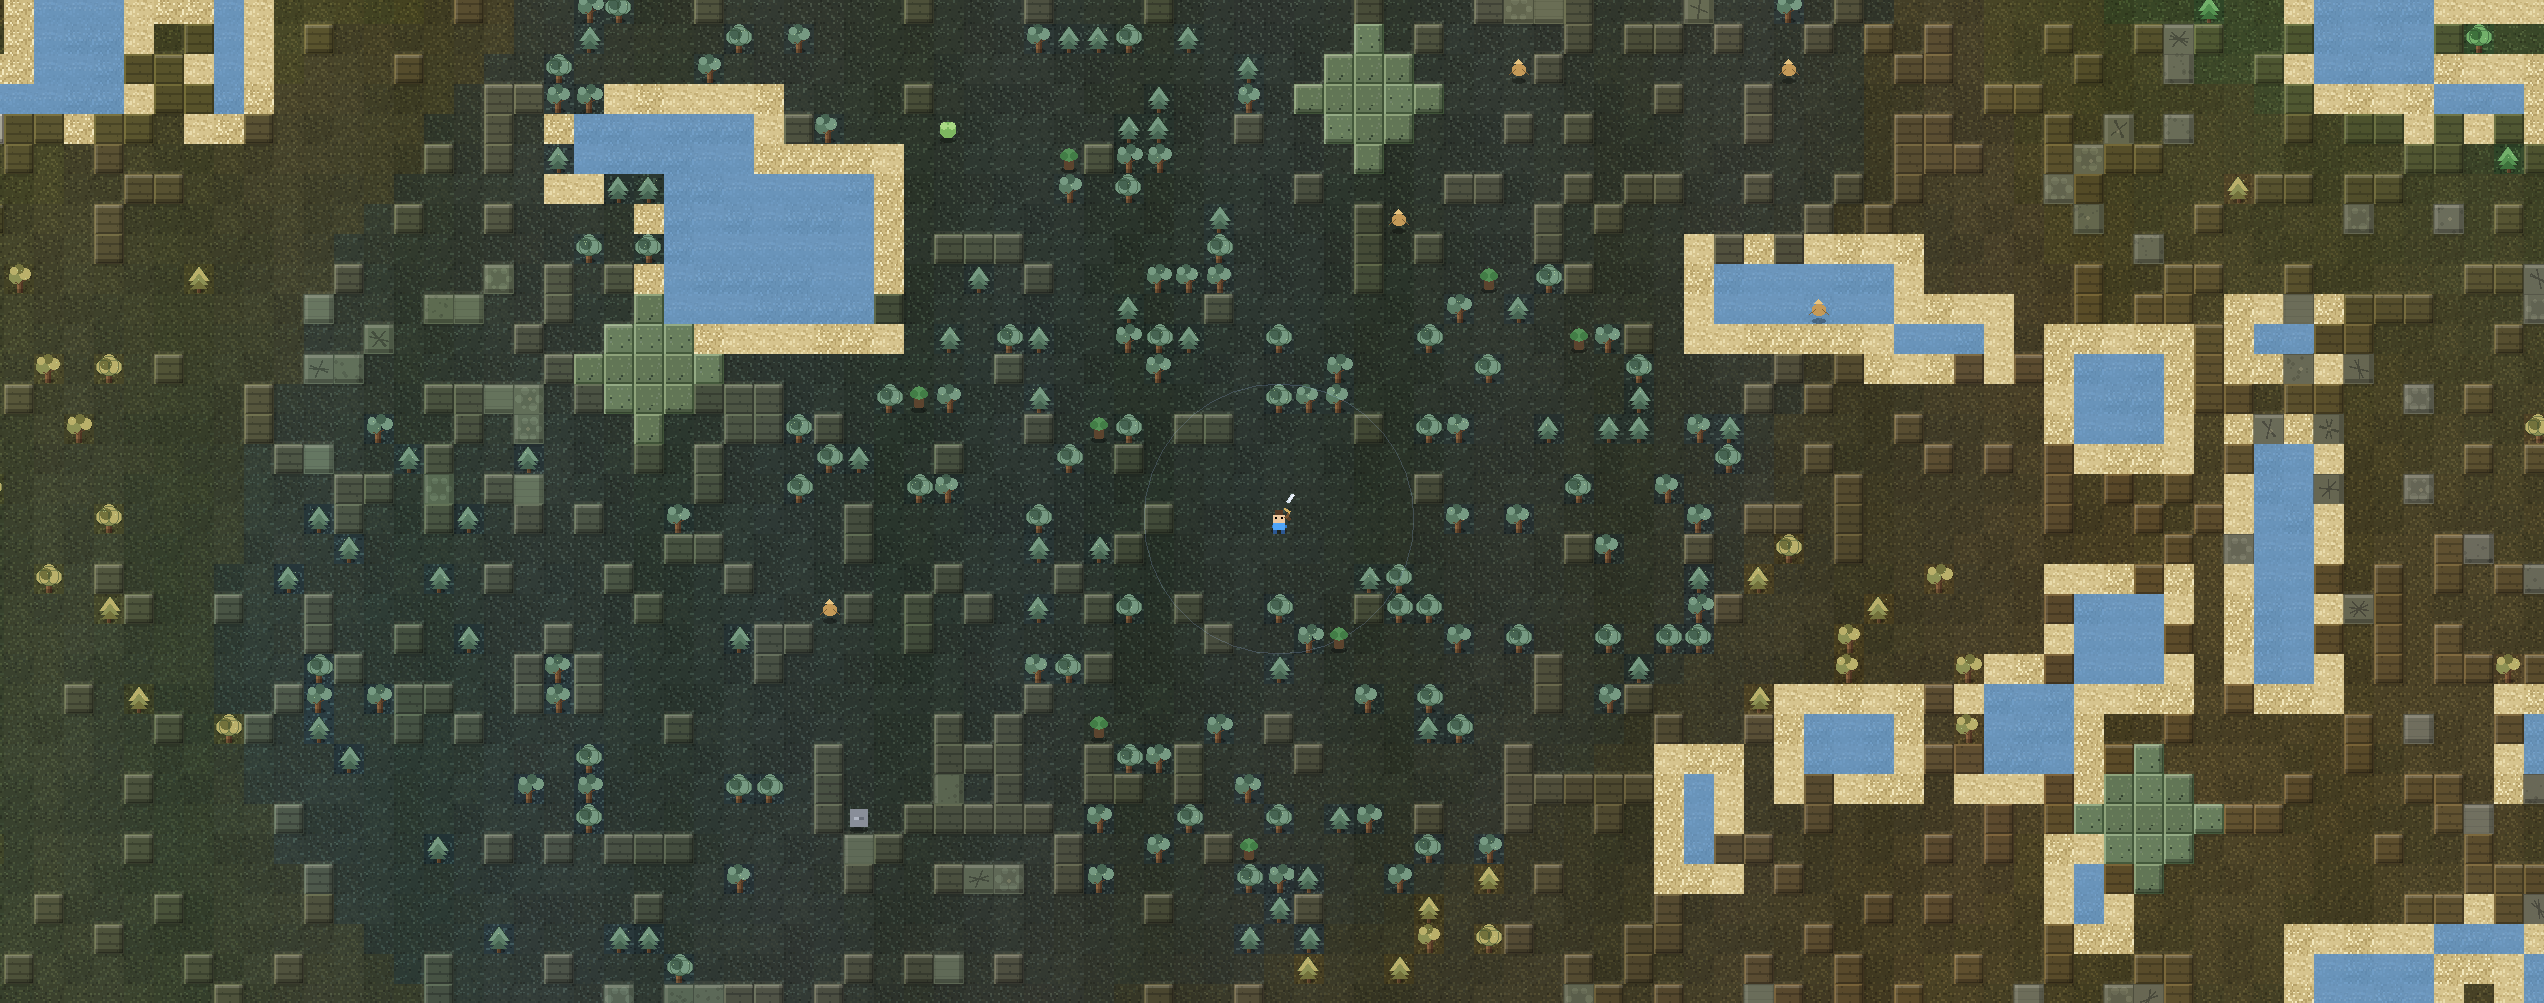
\includegraphics[width=0.95\textwidth]{Bilder/game_preview_clean.png}
    \caption{Visualisierung der generierten Spielwelt mit dynamischer Beleuchtung/Sichtfeld, organischen Seenstrukturen, Strandbereichen und biomabhängigen Kacheltypen. Quelle: Eigene Darstellung (Screenshot des Prototyps, Debug-Overlay entfernt).}
    \label{fig:game_preview}
\end{figure}

\subsection{Synthese der Spielelemente}
In Abbildung~\ref{fig:game_preview} werden die Kernmechanismen der prozeduralen Erzeugung deutlich sichtbar:

\begin{itemize}
    \item \textbf{Beobachtungsradius und Sichtfeld:} Der zentrale Bereich um die Spielfigur wird durch ein kreisförmiges Sichtfeld (\textit{Field of View} / Sichtradius) hervorgehoben. Bereiche außerhalb des aktiven Beobachtungsradius werden abgedunkelt, was den Entdeckungscharakter verstärkt.
    \item \textbf{Organische Gewässer und Strand-Overlay:} Die durch den Low-Frequency-Noise-Score in \texttt{lakeMaskAt} erzeugten Seen treten als zusammenhängende, abgerundete Wasserflächen auf. Das in \texttt{render\_engine.cpp} verankerte Strand-Overlay (\texttt{lakeOrAdjacentAt}) erzeugt an den Begehbarkeitsgrenzen zuverlässig helle Sandstrukturen.
    \item \textbf{Vegetation und Wandelemente:} Die Verteilung von Bäumen (\texttt{TileType::Tree}) und unpassierbaren Hindernissen (\texttt{TileType::Wall}) variiert entsprechend der Schwellenwerte (\texttt{wallThreshold}, \texttt{treeThreshold}) der jeweiligen Biome.
    \item \textbf{Landmarken und Strukturen:} Vereinzelt hervorgehobene symmetrische Fliesenmuster (z.\,B. die quadratischen Rauten-Strukturen im oberen Zentrum) belegen das erfolgreiche Stempeln deterministischer Muster bei der Chunk-Initialisierung.
\end{itemize}

\subsection{Artefaktanalyse: Das Phänomen des Biome-Swallowing}
Trotz der optisch ansprechenden, stufenlosen Farbergänzung durch die gewichtete Biom-Mischung (\texttt{biomeTintAtTile}) deckt die praktische Evaluation eine systematische Schwachstelle des gewählten \textit{Biome Blending}-Ansatzes auf.

Da die Gewichtung der Biomfarben über ein $3 \times 3$-Chunk-Umfeld berechnet wird (\texttt{biomeWeights}), besitzen flächenmäßig dominante Nachbarbiome eine überproportionale Strahlkraft auf dazwischenliegende, kleinere Biome. Dieser Effekt wird als **Biome-Swallowing** (Verschlucken von Kleinbiomen) bezeichnet:

\begin{quote}
\textit{Isolierte Phänomenologie:} Besitzt ein einzelner Chunk (z.\,B. eine $8 \times 8$-Wüste mit orangener Grundpalette) eine räumliche Ausdehnung von nur einem Chunk ($1 \times 1$) und liegt unmittelbar zwischen zwei ausgedehnten Biomen wie einem dichten Wald und einer großen Steppe, so dominiert der mathematische Mittelwert der $3 \times 3$-Nachbarschaft. 
\end{quote}

In der Praxis führt dies dazu, dass die Wüste in der Logik (\texttt{biomeTag == 2}) zwar die korrekten Hindernis-Schwellenwerte und Baumverbote besitzt, visuell jedoch durch die Farbinformationen der umliegenden Wald- und Steppen-Chunks grünlich überfärbt wird. Der isolierte Wüsten-Chunk wird farblich „verschluckt“. 

\subsection{Lösungsansätze für kleine Biome}
Um dieses Artefakt in zukünftigen Iterationen zu vermeiden, ohne auf weiche Farbergänge verzichten zu müssen, kommen zwei Ansätze infrage:

\begin{enumerate}
    \item \textbf{Mindestausdehnung von Biomen (\textit{Clustering}):} Bei der Biom-Zuweisung auf Ebene des Chunk-Rasters muss durch eine zelluläre Automaten-Glättung sichergestellt werden, dass Biome stets in zusammenhängenden Clustern von mindestens $2 \times 2$ Chunks auftreten (siehe Kapitel~2.1.3).
    \item \textbf{Nicht-lineare Interpolations-Gewichtung:} Das Gewicht des eigenen Chunks im Zentrum muss bei der Farberechnung deutlich höher gewichtet werden (z.\,B. Faktor 0,6 für den eigenen Chunk und nur 0,4 verteilt auf die 8 Nachbarn), um die visuelle Eigenständigkeit kompakter Biome zu sichern.
\end{enumerate}

\subsection{Performance-Evaluation und Benchmarking}
\label{sec:ergebnisse_performance}

Zur empirischen Überprüfung der Laufzeit- und Speichereffizienz wurde eine automatisierte Benchmark-Routine im Headless-Runner (\texttt{headless\_main.cpp}) implementiert. Über den CLI-Parameter \texttt{--benchmark-world} führt das System eine isolierte Leistungsmessung durch, ohne vom Grafik-Rendering beeinträchtigt zu werden. Tabelle~\ref{tab:performance_summary} fasst die ermittelten Kennzahlen zusammen.

\begin{table}[htbp]
    \centering
    \caption{Übersicht der Performancemessungen und Benchmarks des Generierungs- und Simulationssystems.}
    \label{tab:performance_summary}
    \begin{tabular}{|l|l|r|}
        \hline
        \textbf{Metrik / Messbereich} & \textbf{Parameter / Stichprobe} & \textbf{Ergebnis} \\ \hline
        Chunk-Generierungszeit & $N = 2048$ Chunks ($8 \times 8$) & $\varnothing\,13{,}12\,\mu\text{s}$ (p95: $18{,}50\,\mu\text{s}$) \\ \hline
        Simulationsschritt (\textit{Step Proxy}) & $N = 5000$ Ticks & $\varnothing\,0{,}01\,\text{ms}$ (p95: $0{,}02\,\text{ms}$) \\ \hline
        Speicherbedarf (Sparse vs. Dicht) & 2048 geladene Chunks & $162\,\text{KiB}$ (\texttt{unordered\_map}) vs. $130\,\text{KiB}$ \\ \hline
        Determinismus-Abweichung & 100 Seeds / $518.400$ Tiles & $0{,}0000\,\% \quad (0\text{ Mismatches})$ \\ \hline
    \end{tabular}
\end{table}

\subsubsection{Generierungsgeschwindigkeit und Lazy Loading}
Die Messung der Erzeugungsdauer einzelner $8 \times 8$-Chunks über $2048$ Stichproben ergibt eine durchschnittliche Generierungszeit von nur $13{,}12\,\mu\text{s}$ pro Chunk bei einem 95-Perzentil (\text{p95}) von $18{,}50\,\mu\text{s}$. 

Diese extrem geringe Erzeugungsdauer bestätigt die Effizienz des mehrstufigen Noise-Ansatzes und der optimierten Tile-Zuweisung. Dank dieser Mikrosekunden-Latenz kann das System neue Chunks vollkommen nahtlos beim Betreten durch den Spieler erzeugen (\textit{Lazy Loading}), ohne dass mikroskopische Ruckler (\textit{Frame Drops}) im Render-Thread wahrnehmbar sind.

\subsubsection{Simulationsschritt und Frame-Proxy}
Um die Ausführungsgeschwindigkeit der Kern-Logik (Pfadfindung, Sichtweitenberechnung, Mob-KI und Kollision) zu bestimmen, wurden $5000$ aufeinanderfolgende Simulationsschritte evaluiert:

\begin{itemize}
    \item \textbf{Durchschnittliche Step-Dauer:} $0{,}01\,\text{ms}$ ($\text{p95} = 0{,}02\,\text{ms}$).
    \item \textbf{Durchsatz-Proxy:} Rein logisch bewältigt die Engine theoretisch ca. $73.000$ Simulations-Ticks pro Sekunde (\textit{Step Proxy}). 
\end{itemize}

Das System bietet damit gewaltigen Headroom für die grafische Darstellung im Client und ermöglicht selbst auf leistungsschwacher Hardware eine flüssige Bildrate bei konstanten $60\,\text{FPS}$.

\subsubsection{Speichereffizienz der Hash-Map-Architektur}
Ein entscheidender Architekturentwurf der Spielwelt ist die Speicherung der Chunks in einer \texttt{std::unordered\_map<uint64\_t, Chunk>}. Bei $2048$ aktiven Chunks (was einem sichtbaren Feld von $128 \times 128$ Chunks bzw. $1024 \times 1024$ Fliesen entspricht) beläuft sich der Speicherverbrauch der Hash-Map inklusive Dynamic-Overhead auf ca. $162\,\text{KiB}$. 

Im Vergleich dazu würde ein zweidimensionales, dicht besetztes Array derselben maximalen Spannen etwa $130\,\text{KiB}$ belegen. Der geringfügige Speicher-Overhead von $\approx 32\,\text{KiB}$ für die Hash-Metadaten wird durch den enormen Vorteil aufgewogen, dass die Welt theoretisch unendlich ausgedehnt sein kann, ohne unbesetzte Weltbereiche vorab im Arbeitsspeicher allozieren zu müssen.

\subsubsection{Determinismus und Reproduzierbarkeit}
Für prozedurale Welten ist die exakte Reproduzierbarkeit essenziell. Zur Verifikation wurden $100$ unterschiedliche Zufallssamen (\textit{Seeds}) evaluiert und insgesamt $518.400$ einzelne Kacheln zwischen mehrfachen Generierungsläufen verglichen:

$$\text{Abweichungsrate} = \frac{\text{Anzahl Mismatches}}{\text{Gesamtzahl verglichener Tiles}} = \frac{0}{518.400} = 0{,}0000\,\%$$

Die Fehlerrate liegt exakt bei $0{,}00\,\%$. Dies beweist, dass sowohl das Noise-Cascading für Höhen und Biome als auch der Manhattan-Carver für Pfade vollständig deterministisch arbeiten und keine unkontrollierten Nebeneffekte oder Zustandsspeicher-Lohnartefakte vorliegen.

\subsection{Kritische Diskussion und Limitationen}
\label{sec:ergebnisse_diskussion}

Die empirischen und visuellen Befunde belegen, dass die entwickelte Architektur für prozedurale Welten eine performante, deterministische und visuell ansprechende Spielumgebung bereitstellt. Dennoch ergeben sich aus den gewählten Entwurfsentscheidungen spezifische Kompromisse und methodische Grenzen, die im Folgenden kritisch gewürdigt werden.

\subsubsection{Vorteile der Architektur}
\begin{itemize}
    \item \textbf{Nahtlose Performanz und Ladezeitfreiheit:} Durch die Kombination aus Mikrosekunden-Chunk-Generierung ($\varnothing\,13{,}12\,\mu\text{s}$) und bedarfsgesteuertem \textit{Lazy Loading} entstehen im Spielverlauf keinerlei spürbare Ladezeiten oder Unterbrechungen (\textit{Stuttering}), wenn der Spieler neue Kartenbereiche erschließt.
    \item \textbf{Garantierte Pfad-Topologie:} Der mathematisch strikte *Manhattan-Carver* garantiert zu $100\,\%$, dass die kritische Traverse zwischen Startpunkt (\texttt{spawn\_}) und Ziel (\texttt{exit\_}) nicht durch Hindernisse blockiert werden kann. Unlösbare Welt-Instanzen werden dadurch deterministisch ausgeschlossen.
    \item \textbf{Minimaler Initial-Speicherbedarf:} Dank der spärlich besetzten Hash-Map-Architektur (\texttt{std::unordered\_map}) belegt die Welt beim Spielstart nur den Speicherplatz der unmittelbar benötigten Initial-Chunks ($\approx 162\,\text{KiB}$ bei 2048 Chunks), anstatt riesige 2D-Arrays vorab im RAM zu reservieren.
\end{itemize}

\subsubsection{Identifizierte Schwachstellen und Limitationen}
\begin{itemize}
    \item \textbf{Geometrische Künstlichkeit des Manhattan-Carvers:} Da der Pfad-Einkerber Kacheln entlang rechtwinkliger Koordinatendifferenzen aufbricht, neigt die Logik zur Bildung auffälliger „L-Shapes“ (rechtwinklige Gänge). In offenem Terrain (z.\,B. Wiese oder Wüste) wirken diese harten $90^\circ$-Achsenbrüche stellenweise unnatürlich und brechen die organische Anmutung der Noise-Generierung.
    \item \textbf{Beschränkung auf flaches 2D-Raster:} Das System arbeitet auf einem rein zweidimensionalen Gitter. Echte Höhenunterschiede, Plateaus, Höhlensysteme auf mehreren Ebenen oder Verdeckungslogiken (z.\,B. Rampen oder Brücken) können ohne Erweiterung um ein $Z$-Achsengitter oder Iso-Layer nicht abgebildet werden.
    \item \textbf{Unbegrenztes RAM-Wachstum ohne Chunk-Unloading:} Obwohl der Einstiegsspeicherbedarf minimal ist, besitzt der aktuelle Chunk-Cache in \texttt{world.cpp} keinen Entlademechanismus (z.\,B. \textit{Least Recently Used} / LRU-Unloading). Besucht ein Spieler in einer extrem langen Sitzung hunderttausende Chunks, wächst die \texttt{unordered\_map} kontinuierlich an.
    \item \textbf{Farb-Absorption bei Kleinbiomen (\textit{Biome-Swallowing}):} Wie in Abschnitt~\ref{sec:ergebnisse_visuell} analysiert, führt das räumlich gewichtete \textit{Biome Blending} über $3 \times 3$ Chunks dazu, dass isolierte Einzel-Chunks ($1 \times 1$) farblich von ihren dominanten Nachbarbiomen überstrahlt werden.
\end{itemize}

\section{Evaluation des RL-Trainings}
\label{sec:evalRL}

Dieser Abschnitt evaluiert die trainierten RL-Verfahren hinsichtlich Erfolgsquote, Pfadeffizienz und Robustheit gegenüber den ungelernten Referenzpunkten aus Abschnitt~\ref{sec:methodik_baselines}. Datengrundlage sind sieben unabhängige Trainingsläufe je Modell, ausgewertet auf dem in Abschnitt~\ref{sec:methodik_protokoll} definierten Testset A.

\subsection{Erfolgsquote der trainierten Verfahren}
\label{sec:eval_sr}
Die Erfolgsquote ist die zentrale Metrik zur Beurteilung, ob ein Verfahren die Navigationsaufgabe überhaupt löst. Abbildung~\ref{fig:eval_sr} stellt die beiden trainierten Modelle in jeweils zwei Auswertungsmodi, deterministisch und stochastisch, den ungelernten Referenzpunkten gegenüber.

\begin{figure}[htbp]
    \centering
    
\includegraphics[width=0.98\textwidth]{Bilder/eval_erfolgsquote.png}
    \caption{Evaluation -- Erfolgsquote der trainierten Verfahren und der Referenzpunkte auf Testset A, eigene Darstellung.}
    \label{fig:eval_sr}
\end{figure}

Das LSTM-PPO-Modell erreicht in der stochastischen Auswertung eine mittlere Erfolgsquote von 65,7\,\%. Über die sieben Durchläufe hinweg liegt die Standardabweichung bei 12,4 Prozentpunkten, die Einzelwerte schwanken zwischen 50,0\,\% und 84,0\,\%. Im deterministischen Modus bricht die Leistung massiv ein: Die Quote fällt auf magere 29,1\,\% $\pm$ 8,0.

Beim MLP-PPO-Verfahren fällt das Bild schwächer aus als beim LSTM. Unter dem identischen Standardprotokoll (siehe Abschnitt~\ref{sec:methodik_protokoll}) erreicht das Modell stochastisch ausgewertet auf Testset A 33,5\,\% $\pm$ 25,5 und auf Testset B 35,8\,\% $\pm$ 30,5. Die Streuung zwischen den sieben Seeds fällt damit mehr als doppelt so hoch aus wie beim LSTM, die Einzelwerte auf Testset A reichen von 4,0\,\% bis 65,2\,\%. Deterministisch ausgewertet scheitert das Netz vollständig: Über alle sieben Läufe und alle 70 Messpunkte der späten Trainingsphasen hinweg liegt die Erfolgsquote bei exakt 0,0\,\%. Dieser deterministische Wert stammt weiterhin aus den Zwischenevaluationen des Trainings, da das kanonische Protokoll aktuell ausschließlich den stochastischen Modus misst.

Der Systemvergleich fällt damit eindeutig aus: Die rekurrente LSTM-Architektur schlägt das gedächtnislose MLP-Netz deutlich. Im deterministischen Modus ist der Unterschied absolut, knapp jede dritte Episode gelöst gegenüber keiner einzigen. Im stochastischen Modus schrumpft der Vorsprung zwar auf rund 32 Prozentpunkte, und die starken Schwankungen des MLP-Modells sorgen für Überschneidungen einzelner Läufe. Das LSTM bleibt dennoch das klar überlegene Verfahren, wobei Abschnitt~\ref{sec:eval_hyperparameter} diesen Vorsprung noch einordnet.

Bei nur sieben Läufen je Architektur und einer Standardabweichung von 25,5 Prozentpunkten beim MLP-Modell stellt sich die Frage, ob dieser Unterschied statistisch belastbar ist oder in der Streuung der kleinen Stichprobe verschwindet. Ein Welch-Test auf die sieben Erfolgsquoten je Verfahren (Testset A, stochastisch) weist den Unterschied als signifikant aus ($t(8{,}7) = 3{,}00$, $p = 0{,}016$), ein verteilungsfreier Mann-Whitney-U-Test bestätigt dies unabhängig von Normalverteilungsannahmen ($U = 41$, $p = 0{,}038$). Die Effektstärke fällt mit Cohens $d = 1{,}6$ groß aus. Auf Testset B liegt der Welch-Test ebenfalls im signifikanten Bereich ($p = 0{,}038$), der Mann-Whitney-Test knapp darüber ($p = 0{,}053$) — auf dem Holdout-Set ist der Befund also weniger robust als auf Testset A. Die einzelnen 95\,\%-Konfidenzintervalle überschneiden sich zwar teilweise (LSTM: $[54{,}2; 77{,}2]$, MLP: $[9{,}9; 57{,}1]$), was bei einem Vergleich zweier einzelner Intervalle leicht als Beleg gegen Signifikanz gelesen werden könnte; das Konfidenzintervall der Differenz selbst schließt die Null jedoch nicht ein ($[7{,}8; 56{,}6]$). Der gemessene Vorsprung des LSTM ist damit trotz der geringen Stichprobengröße nach gängigen Kriterien statistisch abgesichert, auf Testset A deutlicher als auf Testset B.

\subsection{Pfadeffizienz derselben Verfahren}
\label{sec:eval_eff}
Nur am Ausgang anzukommen, reicht als Bewertungskriterium nicht aus, wichtig ist auch der Weg dorthin. Abbildung~\ref{fig:eval_eff} zeigt daher die Pfadeffizienz. Sie berechnet sich aus dem Verhältnis zwischen dem per Breitensuche (siehe Abschnitt~\ref{sec:grundlagen_bfs}) ermittelten kürzesten Weg und den vom Agenten tatsächlich gelaufenen Schritten. Ein Wert von 1,0 markiert das Optimum.

\begin{figure}[htbp]
    \centering
    
\includegraphics[width=0.9\textwidth]{Bilder/eval_pfadeffizienz.png}
    \caption{Evaluation -- Pfadeffizienz der Verfahren in derselben Achsenordnung, eigene Darstellung.}
    \label{fig:eval_eff}
\end{figure}

Das BFS-Optimum liegt auf dem verwendeten Testset im Schnitt bei 40,1 Schritten. Das trainierte LSTM-Modell benötigt für eine erfolgreiche Episode dagegen durchschnittlich 1429 Schritte, das entspricht einer Pfadeffizienz von lediglich 0,049. Der Agent läuft damit im Schnitt einen Weg, der mehr als 35-mal so lang ist wie nötig. Für das MLP-Modell liegt inzwischen ein vergleichbarer Wert vor: Bei durchschnittlich 1084 Schritten je erfolgreicher Episode ergibt sich eine Pfadeffizienz von 0,067 und damit ein höherer Wert als beim LSTM. Dieser Befund ist mit Vorsicht zu lesen, da die Kennzahl nur über die erfolgreichen Episoden gemittelt wird, wie der folgende Absatz zum Selektionseffekt zeigt: Bei einer Erfolgsquote von nur 33,5\,\% löst das MLP-Modell bevorzugt die leichten Seeds, was die Effizienz künstlich anhebt.

Aufschlussreich wird der Blick auf die Referenzverfahren aus Abschnitt~\ref{sec:methodik_baselines}. Der ungelernte Kompass-Agent mit einem Zufallsanteil von $\varepsilon=0{,}3$ erreicht eine Effizienz von 0,177 und ist damit gut dreimal so wegeffizient wie das trainierte LSTM-Netz, auch wenn er dabei eine knapp 14 Prozentpunkte niedrigere Erfolgsquote in Kauf nimmt. Das überraschendere Ergebnis liefert der $\varepsilon=0{,}8$-Kompass: Er übertrifft das trainierte Modell nicht nur bei der Erfolgsquote, sondern mit einer Pfadeffizienz von 0,094 gleichzeitig auch bei der Weglänge.

Ein leichter Selektionseffekt ist hierbei zu berücksichtigen: In die Pfadeffizienz fließen nur jene Episoden ein, bei denen der Ausgang gefunden wurde. Verfahren, die oft scheitern, wobei die gescheiterten Versuche meist sehr lange Irrwege sind, stehen dadurch statistisch etwas besser da, als sie eigentlich sind. Das erklärt den starken Kompass jedoch nicht vollständig. Die bittere Erkenntnis bleibt: Das Training führt zwar ans Ziel, aber alles andere als auf direktem Weg.

\subsection{Die Determinismus-Lücke}
\label{sec:eval_determinismus}
Beide Netzarchitekturen wurden in zwei Modi ausgewertet: deterministisch, wobei stets die wahrscheinlichste Aktion gewählt wird, und stochastisch, wobei die Aktion aus der Wahrscheinlichkeitsverteilung gezogen wird. Der Unterschied zwischen beiden Auswertungen ist enorm, wie Abbildung~\ref{fig:eval_det} für jeden einzelnen Durchlauf zeigt.

\begin{figure}[htbp]
    \centering
    
\includegraphics[width=0.85\textwidth]{Bilder/eval_det_stoch.png}
    \caption{Evaluation -- Erfolgsquote desselben Modellstands in deterministischer und stochastischer Auswertung, eigene Darstellung.}
    \label{fig:eval_det}
\end{figure}

Beim LSTM-PPO klafft zwischen den beiden Modi eine Lücke von durchschnittlich 39,4 Prozentpunkten. Dieses Phänomen tritt konsequent in jedem der sieben Läufe auf: Kein einziger Lauf schneidet deterministisch besser ab als stochastisch. Beim MLP-PPO ist diese Lücke sogar maximal, da der deterministische Modus durchgehend bei null Prozent verharrt.

Das ist ein unbequemer Befund. Die gemessene Erfolgsquote verdankt sich zu einem beträchtlichen Teil dem puren Zufall beim Ziehen aus der Verteilung, nicht einer verlässlichen, gelernten Route. Bleibt der Zufall aus, bleibt der Agent oft in Sackgassen stecken.

Eine ergänzende Trajektorienanalyse stützt diese Vermutung, ohne sie vollständig zu bestätigen. Für zwanzig Seeds aus Testset A (Modell \texttt{v12\_s1}, Distanz 35--45, Schrittlimit 1500 statt der vollen 4000, aus Zeitgründen) richtet sich die deterministische Politik nur in 16,2\,\% der Schritte nach der BFS-optimalen Richtung, die stochastische in 23,4\,\%. Von den 13 gescheiterten deterministischen Episoden erschöpfen 9 das volle Schrittlimit, ohne durch einen erkennbaren Abbruch früher zu enden -- der Agent bewegt sich bis zum Limit weiter, ohne dem Ziel näherzukommen. Einzelne Positionen werden dabei extrem häufig erneut besucht, in einem Fall 161-mal innerhalb von 1500 Schritten. Überraschend liegt die durchschnittliche Zahl mehrfach besuchter Positionen jedoch beim stochastischen Modus höher (90,3 gegenüber 58,5): Der Zufallsanteil erzeugt viele kurze Vor-und-Zurück-Bewegungen, während die deterministische Politik seltener, dafür aber in einzelnen Positionen deutlich hartnäckiger feststeckt. Die einfache Erklärung \glqq Zufall befreit aus der Sackgasse\grqq{} trifft den Befund damit nur teilweise; robuster ist die geringere Optimalausrichtung der deterministischen Politik.

\subsection{Einordnung gegenüber den Referenzpunkten}
\label{sec:eval_einordnung}
Um das Geleistete ins Verhältnis zu setzen, trägt Abbildung~\ref{fig:eval_tradeoff} die beiden Hauptmetriken, Erfolgsquote und Pfadeffizienz, gegeneinander auf.

\begin{figure}[htbp]
    \centering
    
\includegraphics[width=0.9\textwidth]{Bilder/eval_zielkonflikt.png}
    \caption{Evaluation -- Erfolgsquote gegen Pfadeffizienz für alle Verfahren, eigene Darstellung.}
    \label{fig:eval_tradeoff}
\end{figure}

Die fünf Varianten der Kompass-Heuristik aus Abschnitt~\ref{sec:methodik_baselines} ziehen im Diagramm eine zusammenhängende Kurve: Je höher der Zufallsanteil $\varepsilon$ bis zu $0{,}8$, desto höher die Erfolgsquote, aber desto geringer die Pfadeffizienz. Auffällig ist die Position des trainierten Modells: Es liegt vollständig unterhalb dieser Heuristik-Kurve.

Besonders hart fällt der direkte Vergleich mit dem $\varepsilon=0{,}8$-Kompass aus. Dieser schlägt das LSTM-Netzwerk doppelt: bei der Erfolgsquote mit 88,8\,\% gegenüber 65,7\,\% und bei der Effizienz mit 0,094 gegenüber 0,049. Das wiegt umso schwerer angesichts dessen, was der Kompass eigentlich ist: eine primitive Heuristik, die nur Luftlinien-Richtungen kennt, Wände ignoriert und stumpf gegen Hindernisse rennt, bis der Zufall sie befreit.

Dass ein kartenblindes Verfahren ohne Trainingsphase zuverlässiger und direkter ins Ziel findet als ein Agent, der über 2,2 Millionen Zeitschritte optimiert wurde, ist die zentrale Pointe dieser Auswertung. Das ändert nichts daran, dass das LSTM besser lernt als das MLP. Für die Beurteilung, wie leistungsfähig Reinforcement Learning für dieses spezifische Problem tatsächlich ist, bleibt es jedoch ein starker Dämpfer.

\subsection{Wirksamkeit der Hyperparameter}
\label{sec:eval_hyperparameter}
Abseits der großen Metriken liefert der Blick in die Trainingshistorie Erkenntnisse darüber, welche Parameter das Training tatsächlich beeinflussten und welche nicht. Tabelle~\ref{tab:hyperparameter_wirkung} fasst die belegten Stellschrauben zusammen, die vollständige Hyperparameter-Konfiguration findet sich in Tabelle~\ref{tab:parameter_training}.

\begin{table}[htbp]
    \centering
    \caption{Belegte Wirkung einzelner Parameterentscheidungen}
    \label{tab:hyperparameter_wirkung}
    \begin{tabular}{p{2.9cm}p{2.4cm}p{7.9cm}}
        \hline
        \textbf{Parameter} & \textbf{Gewählt} & \textbf{Belegte Wirkung} \\
        \hline
        \texttt{ent\_coef} & $0{,}05$ & Ein Versuch mit $0{,}01$ scheiterte komplett; der Agent fand den Ausgang nicht mehr. Dies war der Parameter mit dem größten messbaren Effekt. \\
        \texttt{n\_steps} & $256$ & Bei $512$ verschwanden die Gradienten im Backpropagation-Through-Time-Verfahren und das Lernsignal brach zusammen. \\
        \texttt{batch\_size} & $8$ (LSTM) & Ein Wert von $64$ destabilisierte den Critic spürbar (84\,\% vs. 48\,\% Erfolgsquote bei 150.000 Schritten). \\
        Curriculum-Gate & doppelt & Der Wechsel von einem reinen Zeit-Limit auf ein Gate aus Leistung \textit{oder} Budget behob drastische Leistungseinbrüche. \\
        PBRS-Puffer & $80$ & Ein zu kleiner Puffer ($20$) führte außerhalb der Zone zu falschem Shaping und zerstörte die gelernte Strategie. \\
        \texttt{vf\_coef} & $0{,}5$ & Eine Erhöhung auf $1{,}0$ wurde getestet, brachte aber nachweislich keine Verbesserung. \\
        \hline
    \end{tabular}
\end{table}

Aus diesen Daten lassen sich zwei Erkenntnisse ableiten. Erstens wird das Trainingsergebnis von wenigen Parametern dominiert: Der Entropie-Koeffizient, also der Zwang zum Ausprobieren neuer Aktionen, ist essenziell, während viele andere Werte kaum messbare Veränderungen brachten. Zweitens halfen erfolgreiche Anpassungen fast ausschließlich dabei, die Exploration zu fördern oder instabile Gradienten zu stabilisieren, nicht aber dabei, das Netz an sich leistungsfähiger zu machen.

Eine Leerstelle bleibt die Netzgröße (siehe Abschnitt~\ref{sec:impl_rl_netze}). Die rekurrente Schicht mit 256 Einheiten wurde nie in einer sauberen Ablationsstudie gegen andere Größen getestet. Ein Versuch mit 512 Einheiten sah zwischenzeitlich vielversprechend aus, lief jedoch nie durch das Testset. Welche Größe hier tatsächlich optimal wäre, lässt sich aus den vorliegenden Daten nicht seriös beantworten.

Damit eng verwandt ist eine Einschränkung der Vergleichbarkeit zwischen den beiden Architekturen selbst. Wie in Abschnitt~\ref{sec:impl_rl_netze} dargestellt, besitzt das LSTM-Modell mit 1.038.917 Parametern gut viermal so viele trainierbare Gewichte wie das MLP-Modell mit 250.629 Parametern, da beide Netze mit dem in der Bibliothek vorgesehenen Standardaufbau trainiert wurden und nicht mit kapazitätsangeglichenen Architekturen. Der in Abschnitt~\ref{sec:eval_sr} gemessene Vorsprung des LSTM ließe sich daher nicht allein auf die Rekurrenz zurückführen, sondern könnte teilweise auch aus der schlicht größeren Netzkapazität stammen. Ein Modellvergleich mit angeglichener Parameterzahl müsste in einer eigenen Ablationsstudie erfolgen, was im Rahmen dieser Arbeit aus Zeitgründen ausgeklammert werden soll. Der zentrale Befund, dass die Kompass-Heuristik beide trainierten Verfahren bei Erfolgsquote und Pfadeffizienz übertrifft (siehe Abschnitt~\ref{sec:eval_einordnung}), bleibt von dieser Einschränkung unberührt, da er unabhängig vom internen Architekturvergleich zwischen LSTM und MLP gilt.

Zum Schluss zeigt das Curriculum (siehe Abschnitt~\ref{sec:impl_rl_pipeline}) ungeschminkt die Grenzen des Modells: In den Trainingsphasen 3 und 4 sollte der Agent bestimmte Erfolgsquoten von 70\,\% und 60\,\% erreichen, um die Phase regulär abzuschließen. In keinem der sieben Läufe ist das gelungen. Die Phasen endeten ausschließlich, weil das feste Schrittbudget aufgebraucht war. Die gewünschte Zielleistung lag außerhalb dessen, was die Architektur auf dieser Distanz leisten konnte.

%%%%%%%%%%%%%%%%%%%%%%%%%%%%%%%%%%%%%%%%%%%%%%%%%%%%%%%%%%%%%%%%
% BEGIN: kapitel/07_fazit.tex
%%%%%%%%%%%%%%%%%%%%%%%%%%%%%%%%%%%%%%%%%%%%%%%%%%%%%%%%%%%%%%%%
\chapter{Fazit und Ausblick}
\label{chap:fazit}

\section{Diskussion der Ergebnisse}
\label{sec:fazit_ergebnisse}
Am Ende der Arbeit steht die Rückkehr zur eingangs formulierten Forschungsfrage aus Abschnitt~\ref{sec:zielsetzung}: wie eine prozedural generierte 2D-Spielwelt aufgebaut sein muss und welches RL-Verfahren darin die besten Navigationsergebnisse liefert. Im Folgenden werden die beiden Teilfragen zunächst getrennt betrachtet. Anschließend werden sie in Abschnitt~\ref{sec:fazit_gesamt} zu einem Gesamtbild zusammengeführt.

\subsection*{Teilfrage 1: Aufbau der Spielwelt}
Die erste Teilfrage betraf die Parameter, die eine generierte Welt fair und für den Agenten lösbar machen. Die Antwort fällt anders aus, als die Fragestellung nahelegt: Die Lösbarkeit entsteht in diesem Setup nicht über ein feingetuntes Parameterfenster, sondern durch eine harte strukturelle Garantie.

Bei jeder Weltinitialisierung wird deterministisch ein achsparalleler Korridor zwischen Startpunkt und Ausgang freigeräumt. Das schließt unlösbare Weltinstanzen kategorisch aus, unabhängig davon, wie dicht oder komplex die restliche Wandstruktur generiert wird. Diese Garantie folgt unmittelbar aus der Konstruktion des Algorithmus: Da \texttt{carveGuaranteedPath} bei jedem \texttt{reset()}-Aufruf deterministisch ausgeführt wird (siehe Abschnitt~\ref{sec:umsetzung_pathing}), kann keine erzeugte Weltinstanz je ohne Verbindung zwischen Start- und Zielpunkt bleiben. Die separat gemessene Determinismus-Abweichung von exakt $0{,}0000\,\%$ (siehe Abschnitt~\ref{sec:ergebnisse_performance}) belegt ergänzend die Reproduzierbarkeit der Weltgenerierung, misst jedoch die Wiederholbarkeit identischer Seeds und nicht die Lösbarkeit selbst.

Die biomabhängigen Wanddichten zwischen 7\,\% und 25\,\% steuern demnach nicht, ob die Welt lösbar ist, sondern lediglich, wie umwegig der Pfad abseits der Hauptroute ausfällt. Dazu kommt eine Generierungsdauer von 13,12 Mikrosekunden je Weltausschnitt und ein Durchsatz von rund 73.000 Simulationsschritten pro Sekunde (siehe Tabelle~\ref{tab:performance_summary}). Diese Performance liefert exakt den Spielraum, den ein paralleles RL-Training benötigt.

Für die erste Teilfrage gilt daher: Die Spielwelt ist fair und lösbar, aber architektonisch erzwungen, nicht parametrisch ausbalanciert.

\subsection*{Teilfrage 2: Wahl des Trainingsverfahrens}
Die zweite Teilfrage zielte auf das RL-Verfahren mit der höchsten Erfolgsquote und den effizientesten Wegen. Unter den trainierten Ansätzen fällt die Antwort eindeutig zugunsten der rekurrenten Architektur aus. Das LSTM-PPO-Modell erreicht in der stochastischen Auswertung eine mittlere Erfolgsquote von 65,7\,\% ($\pm$ 12,4), das MLP-PPO-Modell landet bei 33,5\,\% ($\pm$ 25,5) (siehe Abbildung~\ref{fig:eval_sr}). Deterministisch ausgewertet stehen 29,1\,\% beim LSTM gegen exakt 0,0\,\% beim MLP.

Bemerkenswert ist besonders dieser deterministische Absturz: Ohne Zufallsanteil löst das gedächtnislose MLP-Verfahren in der Zielphase keine einzige Episode (siehe Abbildung~\ref{fig:eval_det}). Stochastisch schrumpft der Abstand zwar auf rund 32 Prozentpunkte, der Vorteil eines verborgenen Gedächtniszustands bleibt jedoch offensichtlich. Mit der partiellen Beobachtbarkeit kommt das LSTM-Netz deutlich besser zurecht. Wie in Abschnitt~\ref{sec:eval_hyperparameter} eingeordnet, ist dieser Vorsprung allerdings nicht sauber von der reinen Netzkapazität zu trennen, da das LSTM gut viermal so viele Parameter besitzt wie das MLP.

Hinsichtlich der Wegeffizienz fällt die Bilanz der trainierten Modelle dagegen ernüchternd aus (siehe Abbildung~\ref{fig:eval_eff}). Für eine erfolgreiche Episode benötigt das trainierte Modell im Schnitt 1429 Schritte, das rechnerische Optimum für den kürzesten Weg liegt bei 40,1 Schritten. Daraus ergibt sich eine Pfadeffizienz von 0,049, die selbst von trivialen Referenzheuristiken um mehr als das Dreifache übertroffen wird. Das beste trainierte Verfahren gewinnt zwar unter den gelernten Ansätzen die Erfolgsquote, scheitert aber an der Wegfindung.

Der Blick auf die Hyperparameter liefert eine klare Erkenntnis (siehe Abschnitt~\ref{sec:eval_hyperparameter}): Wenige Einstellungen dominieren das Training. Der Entropie-Koeffizient entscheidet darüber, ob der Agent das Ziel jemals sieht, weil ein zu niedriger Wert das Navigieren vollständig verlernen lässt. Die wirksamsten Stellschrauben betrafen durchgehend Exploration und Gradientenstabilität, nicht die Kapazität oder Tiefe der neuronalen Netze.

\section{Fazit}
\label{sec:fazit_gesamt}

\subsection{Beitrag der Weltgenerierung (Laurin)}
\label{sec:fazit_weltgenerierung}
Im Rahmen dieser Arbeit wurde ein vollständiges, hochperformantes System zur prozeduralen Generierung unendlicher 2D-Spielwelten auf Basis von C++ und Raylib entworfen und implementiert.

\begin{itemize}
    \item \textbf{Synthese aus Rauschen und Pfadgarantie:} Durch die Kombination mehrstufiger \textit{Value-Noise}-Gitter mit dem maßgeschneiderten, geglätteten \textit{Manhattan-Carver} konnte der Zielkonflikt zwischen organisch wirkenden Landschaften und deterministisch garantierter Begehbarkeit gelöst werden. Unlösbare Welt-Instanzen werden systematisch ausgeschlossen.
    \item \textbf{Hohe Speicher- und Laufzeiteffizienz:} Die Architektur nutzt eine bedarfsgesteuerte Chunk-Verwaltung (\textit{Lazy Loading}) mit einer $8 \times 8$-Kachelstruktur in Kombination mit einer spärlich besetzten Hash-Map (\texttt{std::unordered\_map}). Die Benchmarks bestätigen eine Chunk-Generierungszeit von durchschnittlich $13{,}12\,\mu\text{s}$ und einen minimalen Initialspeicherbedarf von ca. $162\,\text{KiB}$.
    \item \textbf{Visuelle und funktionale Kohärenz:} Das Entkoppeln der logischen Datenhaltung von der visuellen Darstellung ermöglichte dynamische Effekte wie stufenloses \textit{Biome Blending} sowie das nahtlose Ableiten von Strand-Overlays an Seen-Rändern im Render-Pfad, ohne den Speicheraufwand pro Chunk zu erhöhen.
    \item \textbf{Vollständiger Determinismus:} Mit einer Abweichungsquote von $0{,}0000\,\%$ bei über $500.000$ verglichenen Kacheln konnte die exakte Reproduzierbarkeit der Weltgenerierung über individuelle Welt-Seeds nachgewiesen werden.
\end{itemize}

Die gestellten Anforderungen an Verlässlichkeit, Performanz und Ästhetik wurden damit vollumfänglich erfüllt.

\subsection{Gesamtbild (gemeinsam)}
\label{sec:fazit_gesamtbild}
Beide Projektteile, die Entwicklung der prozeduralen Welt und das Training der Agenten, sind für sich genommen funktional und abgeschlossen. Der eigentliche Ertrag der Arbeit liegt jedoch nicht in diesen Einzelergebnissen, sondern in ihrem Zusammenspiel.

Der auffälligste Befund der Evaluation ist, dass eine ungelernte, primitive Heuristik das aufwendig trainierte RL-Modell in beiden Metriken deklassiert: Der $\varepsilon=0{,}8$-Kompass erreicht 88,8\,\% Erfolgsquote gegenüber 65,7\,\% und eine Pfadeffizienz von 0,094 gegenüber 0,049 (siehe Abbildung~\ref{fig:eval_tradeoff}). Diese Heuristik wertet lediglich die Richtungskomponenten zum Ziel aus und geht einen Schritt auf der längeren Achse (siehe Abschnitt~\ref{sec:methodik_baselines}). Sie ist \glqq wandblind\grqq, nutzt keine Pfadfindung und kennt das Layout der Welt nicht.

Genau hier greifen die beiden Teile der Arbeit ineinander. Der garantierte Lösungskorridor wird achsparallel generiert, zuerst entlang der einen, dann entlang der anderen Achse (siehe Abschnitt~\ref{sec:umsetzung_pathing}). Die simple Kompass-Heuristik bewegt sich nach exakt demselben Muster. Es drängt sich der Schluss auf, dass die strukturelle Lösbarkeitsgarantie aus der Weltgenerierung präzise diejenige Wegstruktur in die Karte fräst, die das ungelernte Verfahren instinktiv ausnutzt. Ein perfektes Schloss für einen sehr simplen Schlüssel entsteht damit unbeabsichtigt.

Daraus ergibt sich eine methodische Erkenntnis: Eine Trainingsumgebung, deren Lösbarkeit durch geometrisch reguläre Strukturen erzwungen wird, enthält systembedingte Abkürzungen. Ein Vergleich zwischen gelernten und ungelernten Verfahren misst dann nicht mehr nur die \glqq Intelligenz\grqq\ des Reinforcement Learnings, sondern unweigerlich auch, wie gut sich diese strukturellen Backdoors ausnutzen lassen.

Für die anfängliche Fragestellung bedeutet das: LSTM-PPO bleibt der Gewinner unter den Deep-Learning-Verfahren, die Umgebung ist hochperformant. Bewiesen ist damit jedoch nicht, dass RL diese spezifische Navigationsaufgabe exzellent löst. Belegt ist stattdessen, dass RL unter diesen Rahmenbedingungen schlechter abschneidet als ein triviales Skript. Der Architektur-Mechanismus, der das erklärt, ist damit identifiziert.

\section{Ausblick}
\label{sec:fazit_ausblick}
Aus den Erkenntnissen und methodischen Einschränkungen beider Projektteile ergeben sich Ansatzpunkte für weiterführende Arbeiten, im Folgenden getrennt nach Weltgenerierung und Reinforcement Learning betrachtet.

\subsection{Weltgenerierung (Laurin)}
\label{sec:ausblick_weltgenerierung}
Aus den in Abschnitt~\ref{sec:ergebnisse_diskussion} identifizierten Limitationen sowie den erweiterten Möglichkeiten prozeduraler Spielewelten leiten sich folgende Ansatzpunkte für zukünftige Entwicklungen ab:

\begin{enumerate}
    \item \textbf{Dynamisches Chunk-Unloading (LRU-Cache):} Um bei extrem langen Spielsitzungen ein unbegrenztes Wachstum der Chunk-Map zu verhindern, sollte der Speicher um eine \textit{Least-Recently-Used} (LRU) Entladestrategie erweitert werden. Nicht mehr sichtbare Chunks außerhalb des Spieler-Umkreises können so sicher aus dem RAM entfernt oder auf Datenträger ausgelagert werden.
    \item \textbf{Verbesserung der Pfad-Ästhetik (\textit{A*-Guided Carving}):} Der aktuelle Manhattan-Carver neigt stellenweise zu rechtwinkligen „L-Shapes“. Eine Integration eines A*-Algorithmus mit geglätteter Kostenfunktion (\textit{Bézierte-Gänge} oder Diagonalschneiden) könnte die Wegführung noch organischer in das Noise-Terrain einbetten.
    \item \textbf{Nicht-lineares Biome-Blending:} Zur Vermeidung des \textit{Biome-Swallowing}-Effekts bei $1 \times 1$-Kleinbiomen soll die Farbmischungsmatrix dahingehend angepasst werden, dass der zentrale Chunk ein höheres Eigengewicht erhält oder Biome vorab über zelluläre Automaten geclustert werden.
    \item \textbf{Vertikalität und Multi-Layer-Welten:} Die Erweiterung des 2D-Rasters um eine vereinfachte Höhendimension ($Z$-Ebene) würde das Hinzufügen von unterirdischen Höhlensystemen, mehrstöckigen Dungeons oder fließenden Gewässern (Flüsse) ermöglichen.
\end{enumerate}

\subsection{Reinforcement Learning (Florian)}
\label{sec:ausblick_rl}

\textbf{1. Isolierung der Pfadgarantie:} Die Hypothese, dass die Kompass-Heuristik die achsparallele Generierung ausnutzt, müsste experimentell bewiesen werden. Zukünftige Arbeiten sollten die Lösbarkeit über organische, irreguläre Pfadfindungsalgorithmen sicherstellen, da sich der wahre Leistungsunterschied zwischen Heuristik und RL-Agent erst isolieren lässt, wenn die Umgebung keine offensichtliche Geometrie mehr aufweist (vgl. Listing~\ref{lst:manhattan_carver}).

\textbf{2. Systematische Trajektorienanalyse über alle Modelle:} Eine Stichprobe von zwanzig Seeds an einem einzelnen Modell (Abschnitt~\ref{sec:eval_determinismus}) zeigt bereits eine geringere BFS-Optimalausrichtung im deterministischen Modus (16,2\,\% gegenüber 23,4\,\%) und vereinzelt extreme Positions-Wiederholungen, wobei die anfängliche Vermutung reiner Zwei-Schritt-Schleifen zu einfach war. Offen bleibt eine systematische Untersuchung über alle sieben Modelle und das volle Schrittbudget von 4000 statt der hier aus Zeitgründen verwendeten 1500 Schritte, sowie eine genauere Klassifikation der beobachteten Fest-Steck-Muster.

\textbf{3. Echte Schwierigkeitskalibrierung:} Der direkte Einfluss der Welt-Parameter, etwa Wanddichte, Chunk-Größe und Biom-Verteilung, auf die RL-Metriken bleibt in dieser Arbeit ausgeklammert, weil der Fokus auf dem Vergleich der Trainingsverfahren lag und nicht auf einer Parameterstudie der Weltgenerierung. Eine systematische Variation dieser Werte gegenüber der erreichten Erfolgsquote könnte die erste Teilfrage von einer reinen Aussage über Lösbarkeit zu einer Metrik für Schwierigkeit weiterentwickeln.

\textbf{4. Kapazitätsangeglichene Ablationsstudie:} Wie in Abschnitt~\ref{sec:eval_hyperparameter} benannt, unterscheiden sich LSTM- und MLP-Modell nicht nur in der Rekurrenz, sondern auch in der Parameterzahl. Zukünftige Arbeiten müssten beide Architekturen auf eine vergleichbare Parameterzahl bringen, um den Anteil der Rekurrenz am gemessenen Vorsprung sauber vom Anteil der reinen Netzkapazität zu trennen.


% ---------- Literaturverzeichnis ----------------------------------
% Klassischer BibTeX-Weg (natbib), siehe preamble.tex. Der
% Inhaltsverzeichnis-Eintrag wird hier manuell gesetzt, da \bibliography{}
% -- anders als biblatex' \printbibliography -- die KOMA-Script-Hooks für
% listof/bibliography=totoc nicht automatisch bedient.
\clearpage
\phantomsection
\addcontentsline{toc}{chapter}{Literaturverzeichnis}
\bibliography{literatur}

% ---------- Anhang -------------------------------------------------
\appendix

%%%%%%%%%%%%%%%%%%%%%%%%%%%%%%%%%%%%%%%%%%%%%%%%%%%%%%%%%%%%%%%%
% BEGIN: anhang.tex
%%%%%%%%%%%%%%%%%%%%%%%%%%%%%%%%%%%%%%%%%%%%%%%%%%%%%%%%%%%%%%%%
\chapter{Anhang}
\label{chap:anhang}

%%%%%%%%%%%%%%%%%%%%%%%%%%%%%%%%%%%%%%%%%%%%%%%%%%%%%%%%%%%%%%%%
% END: anhang.tex
%%%%%%%%%%%%%%%%%%%%%%%%%%%%%%%%%%%%%%%%%%%%%%%%%%%%%%%%%%%%%%%%


\end{document}